f\chapter{CvReference}
\section{Image Processing}

Note: The chapter describes functions for image processing and
analysis. Most of the functions work with 2d arrays of pixels. We refer
to the arrays as "images"; however, they do not have to be of type
\cross{IplImage}, they may be \cross{CvMat} or \cross{CvMatND} as well.

\subsection{Gradients, Edges and Corners}

\cvfunc{Sobel}\label{Sobel}
\label{Sobel}
Calculates first, second, third or mixed image derivatives using extended Sobel operator

\cvexp{
void cvSobel(

const CvArr* src,

CvArr* dst,

int xorder,

int yorder,

int aperture\_size=3 );

}{CPP}{Sobel(src,dst,xorder,yorder,aperture\_size = 3)-> None}
\begin{description}
\cvarg{src}{Source image of type CvArr*}
\cvarg{dst}{Destination image}
\cvarg{xorder}{Order of the derivative x}
\cvarg{yorder}{Order of the derivative y}
\cvarg{aperture\_size}{Size of the extended Sobel kernel, must be 1, 3, 5 or 7}
\end{description}

In all cases except 1, an $\texttt{aperture\_size} \times
\texttt{aperture\_size}$ separable kernel will be used to calculate the
derivative. For $\texttt{aperture\_size} = 1$ a $ 3 \times 1$ or $ 1 \times 3$
kernel is used (Gaussian smoothing is not done). There is also special
value \texttt{CV\_SCHARR} (-1) that corresponds to $3\times3$ Scharr
filter that may give more accurate results than $3\times3$ Sobel. Scharr
aperture is

\[ \vecthreethree
{-3}{0}{3}
{-10}{0}{10}
{-3}{0}{3}
\]

for x-derivative or transposed for y-derivative.

The function `cvSobel` calculates the image derivative by convolving the image with the appropriate kernel:

\[
\texttt{dst}(x,y) = \frac{d^{xorder+yorder} \texttt{src}}{dx^{xorder} \cdot dy^{yorder}}
\]

The Sobel operators combine Gaussian smoothing and differentiation
so the result is more or less robust to the noise. Most often,
the function is called with (\texttt{xorder} = 1, \texttt{yorder} = 0,
\texttt{aperture\_size} = 3) or (\texttt{xorder} = 0, \texttt{yorder} = 1,
\texttt{aperture\_size} = 3) to calculate first x- or y- image
derivative. The first case corresponds to

\[ \vecthreethree
{-1}{0}{1}
{-2}{0}{2}
{-1}{0}{1}
\]

kernel and the second one corresponds to
\[ \vecthreethree
{-1}{-2}{-1}
{0}{0}{0}
{1}{2}{1}
\]
or
\[ \vecthreethree
{1}{2}{1}
{0}{0}{0}
{-1}{2}{-1}
\]

kernel, depending on the image origin (\texttt{origin} field of
\texttt{IplImage} structure). No scaling is done, so the destination image
usually has larger by absolute value numbers than the source image. To
avoid overflow, the function requires 16-bit destination image if the
source image is 8-bit. The result can be converted back to 8-bit using
\cross{ConvertScale} or \cross{ConvertScaleAbs} functions. Besides 8-bit images
the function can process 32-bit floating-point images. Both source and
destination must be single-channel images of equal size or ROI size.

\cvfunc{Laplace}\label{Laplace}
\label{Laplace}
Calculates Laplacian of the image

\cvexp{
void cvLaplace(

const CvArr* src,

CvArr* dst,

int aperture\_size=3 );

}{CPP}{Laplace(src,dst,aperture\_size=3)-> None}
\begin{description}
\cvarg{src}{Source image}
\cvarg{dst}{Destination image}
\cvarg{aperture\_size}{Aperture size (it has the same meaning as in \cross{Sobel})}
\end{description}

The function \texttt{cvLaplace} calculates Laplacian of the source image by summing second x- and y- derivatives calculated using Sobel operator:

\[
\texttt{dst}(x,y) = \frac{d^2 \texttt{src}}{dx^2} + \frac{d^2 \texttt{src}}{dy^2}
\]

Specifying \texttt{aperture\_size} = 1 gives the fastest variant that is equal to convolving the image with the following kernel:

\[ \vecthreethree {0}{1}{0}{1}{-4}{1}{0}{1}{0} \]

Similar to \cross{Sobel} function, no scaling is done and the same combinations of input and output formats are supported.

\cvfunc{Canny}\label{Canny}
Implements Canny algorithm for edge detection

\cvexp{
void cvCanny( const CvArr* image,

CvArr* edges,

double threshold1,

double threshold2,

int aperture\_size=3 );

}{CPP}{Canny(image,edges,threshold1,threshold2,aperture\_size=3)-> None}
\begin{description}
\cvarg{image}{Single-channel input image}
\cvarg{edges}{Single-channel image to store the edges found by the function}
\cvarg{threshold1}{The first threshold}
\cvarg{threshold2}{The second threshold}
\cvarg{aperture\_size}{Aperture parameter for Sobel operator (see \cross{Sobel})}
\end{description}

The function \texttt{cvCanny} finds the edges on the input image \texttt{image} and marks them in the output image \texttt{edges} using the Canny algorithm. The smallest of \texttt{threshold1} and \texttt{threshold2} is used for edge linking, the largest - to find initial segments of strong edges.

\cvfunc{PreCornerDetect}\label{PreCornerDetect}
Calculates feature map for corner detection

\cvexp{
void cvPreCornerDetect(

const CvArr* image,

CvArr* corners,

int aperture\_size=3 );

}{CPP}{PreCornerDetect(image,corners,aperture\_size=3)-> None}
\begin{description}
\cvarg{image}{Input image}
\cvarg{corners}{Image to store the corner candidates}
\cvarg{aperture\_size}{Aperture parameter for Sobel operator (see \cross{Sobel})}
\end{description}

The function \texttt{cvPreCornerDetect} calculates the function

\[
D_x^2 D_{yy} + D_y^2 D_{xx} - 2 D_x D_y D_{xy}
\]

where $D_?$ denotes one of the first image derivatives and $D_{??}$ denotes a second image derivative.

The corners can be found as local maximums of the function:

\begin{lstlisting}
// assume that the image is floating-point
IplImage* corners = cvCloneImage(image);
IplImage* dilated_corners = cvCloneImage(image);
IplImage* corner_mask = cvCreateImage( cvGetSize(image), 8, 1 );
cvPreCornerDetect( image, corners, 3 );
cvDilate( corners, dilated_corners, 0, 1 );
cvSubS( corners, dilated_corners, corners );
cvCmpS( corners, 0, corner_mask, CV_CMP_GE );
cvReleaseImage( &corners );
cvReleaseImage( &dilated_corners );
\end{lstlisting}

\cvfunc{CornerEigenValsAndVecs}\label{CornerEigenValsAndVecs}
Calculates eigenvalues and eigenvectors of image blocks for corner detection

\cvexp{
void cvCornerEigenValsAndVecs( \par const CvArr* image,\par CvArr* eigenvv,\par int block\_size,\par int aperture\_size=3 );

}{CPP}{CornerEigenValsAndVecs(image,eigenvv,block\_size,aperture\_size=3)-> None}

\begin{description}
\cvarg{image}{Input image}
\cvarg{eigenvv}{Image to store the results. It must be 6 times wider than the input image}
\cvarg{block\_size}{Neighborhood size (see discussion)}
\cvarg{aperture\_size}{Aperture parameter for Sobel operator (see \cross{Sobel})}
\end{description}

For every pixel The function \texttt{cvCornerEigenValsAndVecs} considers \texttt{block\_size} $\times$ \texttt{block\_size} neigborhood S(p). It calcualtes covariation matrix of derivatives over the neigborhood as:

\[
M = \begin{bmatrix}
\sum_{S(p)}(dI/dx)^2 & \sum_{S(p)}(dI/dx \cdot dI/dy)^2 \\
\sum_{S(p)}(dI/dx \cdot dI/dy)^2 & \sum_{S(p)}(dI/dy)^2
\end{bmatrix}
\]

After that it finds eigenvectors and eigenvalues of the matrix and stores them into destination image in form
$(\lambda_1, \lambda_2, x_1, y_1, x_2, y_2)$ where
\begin{description}
\item[$\lambda_1, \lambda_2$]eigenvalues of $M$; not sorted
\item[$x_1, y_1$]eigenvector corresponding to $\lambda_1$
\item[$x_2, y_2$]eigenvector corresponding to $\lambda_2$
\end{description}

\cvfunc{CornerMinEigenVal}\label{CornerMinEigenVal}
Calculates minimal eigenvalue of gradient matrices for corner detection

\cvexp{
void cvCornerMinEigenVal(

const CvArr* image,

CvArr* eigenval,

int block\_size,

int aperture\_size=3 );

}{CPP}{CornerMinEigenVal(image,eigenval,block\_size,aperture\_size=3)-> None}
\begin{description}
\cvarg{image}{Input image}
\cvarg{eigenval}{Image to store the minimal eigen values. Should have the same size as \texttt{image}}
\cvarg{block\_size}{Neighborhood size (see discussion of \cross{CornerEigenValsAndVecs})}
\cvarg{aperture\_size}{Aperture parameter for Sobel operator (see \cross{Sobel}).}
%  format. In the case of floating-point input format this parameter is the number of the fixed float filter used for differencing
\end{description}

The function \texttt{cvCornerMinEigenVal} is similar to \cross{CornerEigenValsAndVecs} but it calculates and stores only the minimal eigen value of derivative covariation matrix for every pixel, i.e. $min(\lambda_1, \lambda_2)$ in terms of the previous function.

\cvfunc{CornerHarris}\label{CornerHarris}
Harris edge detector

\cvexp{
void cvCornerHarris(

const CvArr* image,

CvArr* harris\_responce,

int block\_size,

int aperture\_size=3,

double k=0.04 );

}{CPP}{CornerHarris(image,harris\_dst,block\_size,aperture\_size=3,k=0.04)-> None}

\begin{description}
\cvarg{image}{Input image}
\cvarg{harris\_responce}{Image to store the Harris detector responces. Should have the same size as \texttt{image}}
\cvarg{block\_size}{Neighborhood size (see discussion of \cross{CornerEigenValsAndVecs})}
\cvarg{aperture\_size}{Aperture parameter for Sobel operator (see \cross{Sobel}).}
% format. In the case of floating-point input format this parameter is the number of the fixed float filter used for differencing
\cvarg{k}{Harris detector free parameter. See the formula below.}
\end{description}

The function \texttt{cvCornerHarris} runs the Harris edge detector on image. Similarly to \cross{CornerMinEigenVal} and \cross{CornerEigenValsAndVecs}, for each pixel it calculates $2\times2$ gradient covariation matrix $M$ over $\texttt{block\_size} \times \texttt{block\_size}$ neighborhood. Then, it stores

\[
det(M) - k \, trace(M)^2
\]

to the destination image. Corners in the image can be found as local maxima of the destination image.

\cvfunc{FindCornerSubPix}\label{FindCornerSubPix}
Refines corner locations

\cvexp{
void cvFindCornerSubPix(

const CvArr* image,

CvPoint2D32f* corners,

int count,

CvSize win,

CvSize zero\_zone,

CvTermCriteria criteria );
}{CPP}{FindCornerSubPix(image,win,zero\_zone,criteria)-> corners}

\begin{description}
\cvarg{image}{Input image}
\cvarg{corners}{Initial coordinates of the input corners and refined coordinates on output}
\cvarg{count}{Number of corners}
\cvarg{win}{Half sizes of the search window. For example, if \texttt{win} =(5,5) then 5*2+1 $\times$ 5*2+1 = 11 $\times$ 11 search window is used}
\cvarg{zero\_zone}{Half size of the dead region in the middle of the search zone over which the summation in formulae below is not done. It is used sometimes to avoid possible singularities of the autocorrelation matrix. The value of (-1,-1) indicates that there is no such size}
\cvarg{criteria}{Criteria for termination of the iterative process of corner refinement. That is, the process of corner position refinement stops either after certain number of iteration or when a required accuracy is achieved. The `criteria` may specify either of or both the maximum number of iteration and the required accuracy}
\end{description}

The function \texttt{cvFindCornerSubPix} iterates to find the sub-pixel accurate location of corners, or radial saddle points, as shown in on the picture below.

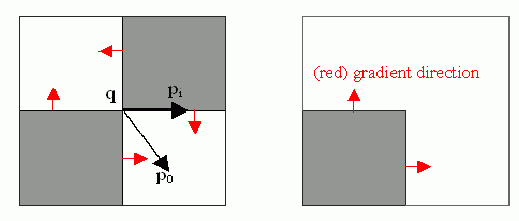
\includegraphics[width=1.0\textwidth]{pics/cornersubpix.png}

Sub-pixel accurate corner locator is based on the observation that every vector from the center $q$ to a point $p$ located within a neighborhood of $q$ is orthogonal to the image gradient at $p$ subject to image and measurement noise. Consider the expression:

\[
\epsilon_i = {DI_{p_i}}^T \cdot (q - p_i)
\]

where ${DI_{p_i}}$ is the image gradient at the one of the points $p_i$ in a neighborhood of $q$. The value of $q$ is to be found such that $\epsilon_i$ is minimized. A system of equations may be set up with $\epsilon_i$ set to zero:

\[
\sum_i(DI_{p_i} \cdot {DI_{p_i}}^T) - \sum_i(DI_{p_i} \cdot {DI_{p_i}}^T \cdot p_i)
\]

where the gradients are summed within a neighborhood ("search window") of $q$. Calling the first gradient term $G$ and the second gradient term $b$ gives:

\[
q = G^{-1} \cdot b
\]

The algorithm sets the center of the neighborhood window at this new center $q$ and then iterates until the center keeps within a set threshold.

\cvfunc{GoodFeaturesToTrack}\label{GoodFeaturesToTrack}
Determines strong corners on image

\cvexp{
void cvGoodFeaturesToTrack(

const CvArr* image

CvArr* eig\_image, CvArr* temp\_image

CvPoint2D32f* corners

int* corner\_count

double quality\_level

double min\_distance

const CvArr* mask=NULL

int block\_size=3

int use\_harris=0

double k=0.04 );

}{CPP}{GoodFeaturesToTrack(image,eig\_image,temp\_image,quality\_level,min\_distance,mask=NULL,block\_size=3,use\_harris=0,k=0.04)-> corners}

\begin{description}
\cvarg{image}{The source 8-bit or floating-point 32-bit, single-channel image}
\cvarg{eig\_image}{Temporary floating-point 32-bit image of the same size as \texttt{image}}
\cvarg{temp\_image}{Another temporary image of the same size and same format as \texttt{eig\_image}}
\cvarg{corners}{Output parameter. Detected corners}
\cvarg{corner\_count}{Output parameter. Number of detected corners}
\cvarg{quality\_level}{Multiplier for the maxmin eigenvalue; specifies minimal accepted quality of image corners.}
\cvarg{min\_distance}{Limit, specifying minimum possible distance between returned corners; Euclidian distance is used.}
\cvarg{mask}{Region of interest. The function selects points either in the specified region or in the whole image if the mask is NULL.}
\cvarg{block\_size}{Size of the averaging block, passed to underlying \cross{CornerMinEigenVal} or \cross{CornerHarris} used by the function}
\cvarg{use\_harris}{If nonzero, Harris operator (\cross{CornerHarris}) is used instead of default \cross{CornerMinEigenVal}}
\cvarg{k}{Free parameter of Harris detector; used only if ($\texttt{use\_harris} != 0$)}
\end{description}

The function \texttt{cvGoodFeaturesToTrack} finds corners with big
eigenvalues in the image. The function first calculates the minimal
eigenvalue for every source image pixel using \cross{CornerMinEigenVal}
function and stores them in \texttt{eig\_image}. Then it performs
non-maxima suppression (only local maxima in $3\times 3$ neighborhood
remain). The next step is rejecting the corners with the minimal
eigenvalue less than
$\texttt{quality\_level} \cdot max(\texttt{eig\_image}(x,y))$
.
Finally, the function ensures that all the corners found are distanced
enough one from another by considering the corners (the most strongest
corners are considered first) and checking that the distance between
the newly considered feature and the features considered earlier
is larger than \texttt{min\_distance}. So, the function removes the
features than are too close to the stronger features.

\cvfunc{ExtractSURF}\label{ExtractSURF}

Extracts Speeded Up Robust Features from image

\cvexp{
void cvExtractSURF( \par const CvArr* image,\par const CvArr* mask,\par CvSeq** keypoints,\par CvSeq** descriptors,\par CvMemStorage* storage,\par CvSURFParams params );
}{CPP}{ExtractSURF(image,mask,storage,params)-> keypoints,descriptors}

\begin{description}
\cvarg{image}{The input 8-bit grayscale image.}
\cvarg{mask}{The optional input 8-bit mask. The features are only found in the areas that contain more than 50\% of non-zero mask pixels.}
\cvarg{keypoints}{The output parameter; double pointer to the sequence of keypoints. This will be the sequence of CvSURFPoint structures:}
\begin{lstlisting}
 typedef struct CvSURFPoint
 {
    CvPoint2D32f pt; // position of the feature within the image
    int laplacian;   // -1, 0 or +1. sign of the laplacian at the point.
                     // can be used to speedup feature comparison
                     // (normally features with laplacians of different signs can not match)
    int size;        // size of the feature
    float dir;       // orientation of the feature: 0..360 degrees
    float hessian;   // value of the hessian (can be used to approximately estimate the feature strengths;
                     // see also params.hessianThreshold)
 }
 CvSURFPoint;
\end{lstlisting}
\cvarg{descriptors}{The optional output parameter; double pointer to the sequence of descriptors; Depending on the params.extended value, each element of the sequence will be either 64-element or 128-element floating-point (\texttt{CV\_32F}) vector. If the parameter is NULL, the descriptors are not computed. }
\cvarg{storage}{Memory storage where keypoints and descriptors will be stored.}
\cvarg{params}{Various algorithm parameters put to the structure CvSURFParams: }
\begin{lstlisting}
 typedef struct CvSURFParams
 {
    int extended; // 0 means basic descriptors (64 elements each),
                  // 1 means extended descriptors (128 elements each)
    double hessianThreshold; // only features with keypoint.hessian larger than that are extracted.
                  // good default value is ~300-500 (can depend on the average
                  // local contrast and sharpness of the image).
                  // user can further filter out some features based on their hessian values
                  // and other characteristics
    int nOctaves; // the number of octaves to be used for extraction.
                  // With each next octave the feature size is doubled (3 by default)
    int nOctaveLayers; // The number of layers within each octave (4 by default)
 }
 CvSURFParams;

 CvSURFParams cvSURFParams(double hessianThreshold, int extended=0); // returns default parameters
\end{lstlisting}
\end{description}

The function cvExtractSURF finds robust features in the image, as
described in
Bay06
. For each feature it returns its location, size,
orientation and optionally the descriptor, basic or extended. The function
can be used for object tracking and localization, image stitching etc. See
\texttt{find\_obj.cpp} demo in OpenCV samples directory.

\cvfunc{GetStarKeypoints}\label{GetStarKeypoints}

Retrieves keypoints using StarDetector algorithm

\cvexp{
CvSeq* cvGetStarKeypoints( \par const CvArr* image,\par CvMemStorage* storage,\par CvStarDetectorParams params=cvStarDetectorParams() );
}{CPP}{GetStarKeypoints(image,storage,params)-> keypoints}

\begin{description}
\cvarg{image}{The input 8-bit grayscale image.}
\cvarg{storage}{Memory storage where keypoints will be stored.}
\cvarg{params}{Various algorithm parameters put to the structure CvStarDetectorParams:}
\begin{lstlisting}
 typedef struct CvStarDetectorParams
 {
    int maxSize; // maximal size of the features detected. The following values
                 // of the parameter are supported:
                 // 4, 6, 8, 11, 12, 16, 22, 23, 32, 45, 46, 64, 90, 128
    int responseThreshold; // threshold for the approximatd laplacian,
                           // used to eliminate weak features
    int lineThresholdProjected; // another threshold for laplacian to eliminate edges
    int lineThresholdBinarized; // another threshold for the feature scale to eliminate edges
    int suppressNonmaxSize; // linear size of a pixel neighborhood for non-maxima suppression
 }
 CvStarDetectorParams;
\end{lstlisting}
\end{description}

The function GetStarKeypoints extracts keypoints that are local
scale-space extremas. The scale-space is constructed by computing
approximate values of laplacians with different sigma's at each
pixel. Instead of using pyramids, a popular approach to save computing
time, all the laplacians are computed at each pixel of the original
high-resolution image. But each approximate laplacian value is computed
in O(1) time regardless of the sigma, thanks to the use of integral
images. The algorithm is based on the paper 
Agrawal08
, but instead
of square, hexagon or octagon it uses 8-end star shape, hence the name,
consisting of overlapping upright and tilted squares.

Each computed feature is represented by the following structure:

\begin{lstlisting}
typedef struct CvStarKeypoint
{
    CvPoint pt; // coordinates of the feature
    int size; // feature size, see CvStarDetectorParams::maxSize
    float response; // the approximated laplacian value at that point.
}
CvStarKeypoint;

inline CvStarKeypoint cvStarKeypoint(CvPoint pt, int size, float response);
\end{lstlisting}

Below is the small usage sample:

\begin{lstlisting}
#include "cv.h"
#include "highgui.h"

int main(int argc, char** argv)
{
    const char* filename = argc > 1 ? argv[1] : "lena.jpg";
    IplImage* img = cvLoadImage( filename, 0 ), *cimg;
    CvMemStorage* storage = cvCreateMemStorage(0);
    CvSeq* keypoints = 0;
    int i;

    if( !img )
        return 0;
    cvNamedWindow( "image", 1 );
    cvShowImage( "image", img );
    cvNamedWindow( "features", 1 );
    cimg = cvCreateImage( cvGetSize(img), 8, 3 );
    cvCvtColor( img, cimg, CV_GRAY2BGR );

    keypoints = cvGetStarKeypoints( img, storage, cvStarDetectorParams(45) );

    for( i = 0; i < (keypoints ? keypoints->total : 0); i++ )
    {
        CvStarKeypoint kpt = *(CvStarKeypoint*)cvGetSeqElem(keypoints, i);
        int r = kpt.size/2;
        cvCircle( cimg, kpt.pt, r, CV_RGB(0,255,0));
        cvLine( cimg, cvPoint(kpt.pt.x + r, kpt.pt.y + r),
            cvPoint(kpt.pt.x - r, kpt.pt.y - r), CV_RGB(0,255,0));
        cvLine( cimg, cvPoint(kpt.pt.x - r, kpt.pt.y + r),
            cvPoint(kpt.pt.x + r, kpt.pt.y - r), CV_RGB(0,255,0));
    }
    cvShowImage( "features", cimg );
    cvWaitKey();
}
\end{lstlisting}

\subsection{Sampling, Interpolation and Geometrical Transforms}

\cvfunc{SampleLine}\label{SampleLine}
Reads raster line to buffer

\cvexp{
int cvSampleLine(

const CvArr* image

CvPoint pt1

CvPoint pt2

void* buffer

int connectivity=8 );

}{CPP}{PYTHON}

\begin{description}
\cvarg{image}{Image to sample the line from}
\cvarg{pt1}{Starting the line point}
\cvarg{pt2}{Ending the line point}
\cvarg{buffer}{Buffer to store the line points; must have enough size to store
$max( |\texttt{pt2.x} - \texttt{pt1.x}|+1, |\texttt{pt2.y} - \texttt{pt1.y}|+1 )$
points in case of 8-connected line and
$ (|\texttt{pt2.x}-\texttt{pt1.x}|+|\texttt{pt2.y}-\texttt{pt1.y}|+1) $
in case of 4-connected line.}
\cvarg{connectivity}{The line connectivity, 4 or 8}
\end{description}

The function \texttt{cvSampleLine} implements a particular case of application of line iterators. The function reads all the image points lying on the line between \texttt{pt1} and \texttt{pt2}, including the ending points, and stores them into the buffer.

\cvfunc{GetRectSubPix}\label{GetRectSubPix}

Retrieves pixel rectangle from image with sub-pixel accuracy

\cvexp{
void cvGetRectSubPix(

const CvArr* src,

CvArr* dst,

CvPoint2D32f center );
}{CPP}{GetRectSubPix(src,dst,center)-> None}

\begin{description}
\cvarg{src}{Source image}
\cvarg{dst}{Extracted rectangle}
\cvarg{center}{Floating point coordinates of the extracted rectangle center within the source image. The center must be inside the image.}
\end{description}

The function \texttt{cvGetRectSubPix} extracts pixels from \texttt{src}:

\[
dst(x, y) = src(x + \texttt{center.x} - (width(\texttt{dst})-1)*0.5, y + \texttt{center.y} - (height(\texttt{dst} )-1)*0.5)
\]

where the values of pixels at non-integer coordinates are retrieved
using bilinear interpolation. Every channel of multiple-channel
images is processed independently. Whereas the rectangle center
must be inside the image, the whole rectangle may be partially
occluded. In this case, the replication border mode is used to get
pixel values beyond the image boundaries.

\cvfunc{GetQuadrangleSubPix}\label{GetQuadrangleSubPix}

Retrieves pixel quadrangle from image with sub-pixel accuracy

\cvexp{
void cvGetQuadrangleSubPix(

const CvArr* src,

CvArr* dst,

const CvMat* map\_matrix );

}{CPP}{GetQuadrangleSubPix(src,dst,map\_matrix)-> None}

\begin{description}
\cvarg{src}{Source image}
\cvarg{dst}{Extracted quadrangle}
\cvarg{map\_matrix}{The transformation $2 \times 3$ matrix $[A|b]$ (see the discussion)}
\end{description}

The function \texttt{cvGetQuadrangleSubPix} extracts pixels from \texttt{src} at sub-pixel accuracy and stores them to \texttt{dst} as follows:

\[
dst(x, y)= src( A_{11} x' + A_{12} y' + b_1, A_{21} x' + A_{22} y' + b_2)
\]

where

\[
x'=\frac{x-(width(dst)-1)}{2}, 
y'=\frac{y-(height(dst)-1)}{2}
\]

and

\[
\texttt{map\_matrix} = \begin{bmatrix}
A_{11} & A_{12} & b_1\\
A_{21} & A_{22} & b_2
\end{bmatrix}
\]

where the values of pixels at non-integer coordinates are retrieved using bilinear interpolation. When the function needs pixels outside of the image, it uses replication border mode to reconstruct the values. Every channel of multiple-channel images is processed independently.


\cvfunc{Resize}\label{Resize}
Resizes image

\cvexp{
void cvResize(

const CvArr* src,

CvArr* dst,

int interpolation=CV\_INTER\_LINEAR );

}{CPP}{Resize(src,dst,interpolation=CV\_INTER\_LINEAR)-> None}

\begin{description}
\cvarg{src}{Source image}
\cvarg{dst}{Destination image}
\cvarg{interpolation}{Interpolation method:
\begin{description}
\cvarg{CV\_INTER\_NN}{nearest-neigbor interpolation}
\cvarg{CV\_INTER\_LINEAR}{bilinear interpolation (used by default)}
\cvarg{CV\_INTER\_AREA}{resampling using pixel area relation. It is preferred method for image decimation that gives moire-free results. In case of zooming it is similar to \texttt{CV\_INTER\_NN} method.}
\cvarg{CV\_INTER\_CUBIC}{bicubic interpolation.}
\end{description}}
\end{description}

The function \texttt{cvResize} resizes image \texttt{src} so that it fits exactly to \texttt{dst}. If ROI is set, the function considers the ROI as supported as usual.

\cvfunc{WarpAffine}\label{WarpAffine}

Applies affine transformation to the image

\cvexp{
void cvWarpAffine(

const CvArr* src,

CvArr* dst,

const CvMat* map\_matrix,

int flags=CV\_INTER\_LINEAR+CV\_WARP\_FILL\_OUTLIERS,

CvScalar fillval=cvScalarAll(0) );

}{CPP}{WarpAffline(src,dst,map\_matrix,flags=CV\_INTER\_LINEAR+CV\_WARP\_FILL\_OUTLIERS,fillval=cvScalarAll(0))-> None}

\begin{description}
\cvarg{src}{Source image}
\cvarg{dst}{Destination image}
\cvarg{map\_matrix}{$2\times 3$ transformation matrix}
\cvarg{flags}{A combination of interpolation method and the following optional flags:
\begin{description}
  \cvarg{CV\_WARP\_FILL\_OUTLIERS}{fill all the destination image pixels. If some of them correspond to outliers in the source image, they are set to `fillval`}
  \cvarg{CV\_WARP\_INVERSE\_MAP}{indicates that \texttt{matrix} is inverse
  transform from destination image to source and, thus, can be used
  directly for pixel interpolation. Otherwise, the function finds
  the inverse transform from \texttt{map\_matrix}.}}
\end{description}
\cvarg{fillval}{A value used to fill outliers}
\end{description}

The function \texttt{cvWarpAffine} transforms source image using the specified matrix:

\[
dst(x',y') = src(x,y)
\]

where

\[
\begin{matrix}
\begin{bmatrix}
x'\\
y'
\end{bmatrix} = \texttt{map\_matrix} \cdot \begin{bmatrix}
x\\
y\\
1
\end{bmatrix} & \mbox{if CV\_WARP\_INVERSE\_MAP is not set}\\
\begin{bmatrix}
x\\
y
\end{bmatrix} = \texttt{map\_matrix} \cdot \begin{bmatrix}
x'\\
y'\\
1
\end{bmatrix}& \mbox{otherwise}
\end{matrix}
\]

The function is similar to \cross{GetQuadrangleSubPix} but they are not exactly the same. \cross{WarpAffine} requires input and output image have the same data type, has larger overhead (so it is not quite suitable for small images) and can leave part of destination image unchanged. While \cross{GetQuadrangleSubPix} may extract quadrangles from 8-bit images into floating-point buffer, has smaller overhead and always changes the whole destination image content.

To transform a sparse set of points, use \cross{Transform} function from cxcore.

\cvfunc{GetAffineTransform}\label{GetAffineTransform}

Calculates affine transform from 3 corresponding points

\cvexp{
CvMat* cvGetAffineTransform(

const CvPoint2D32f* src,

const CvPoint2D32f* dst, 

CvMat* map\_matrix );
}{CPP}{GetAffineTransform(src,dst,map\_matrix)-> None}

\begin{description}
\cvarg{src}{ Coordinates of 3 triangle vertices in the source image}
\cvarg{dst}{ Coordinates of the 3 corresponding triangle vertices in the destination image}
\cvarg{map\_matrix}{ Pointer to the destination $2 \times 3$ matrix}
\end{description}

The function cvGetAffineTransform calculates the matrix of an affine transform such that:

\[
\begin{bmatrix}
x'_i\\
y'_i
\end{bmatrix}
=
\texttt{map\_matrix}
\cdot
\begin{bmatrix}
x_i\\
y_i\\
1
\end{bmatrix}
\]

where

\[
dst(i)=(x'_i,y'_i),
src(i)=(x_i, y_i),
i=0,1,2
\]

\cvfunc{2DRotationMatrix}\label{2DRotationMatrix}

Calculates affine matrix of 2d rotation

\cvexp{
CvMat* cv2DRotationMatrix(

CvPoint2D32f center,

double angle,

double scale,

CvMat* map\_matrix );
}{CPP}{2DRotationMatrix(center,angle,scale,map\_matrix)-> None}

\begin{description}
\cvarg{center}{Center of the rotation in the source image}
\cvarg{angle}{The rotation angle in degrees. Positive values mean couter-clockwise rotation (the coordiate origin is assumed at top-left corner)}
\cvarg{scale}{Isotropic scale factor}
\cvarg{map\_matrix}{Pointer to the destination $2\times 3$ matrix}
\end{description}

The function \texttt{cv2DRotationMatrix} calculates matrix:

\[
\begin{bmatrix}
a & \beta & (1-a) \cdot \texttt{center.x} - \beta \cdot \texttt{center.y} \\
\beta - 1 & a & \beta \cdot \texttt{center.x} - (1-a) \cdot \texttt{center.y}
\end{bmatrix}
\]

where

\[
a = \texttt{scale} \cdot cos(\texttt{angle}), \beta = \texttt{scale} \cdot sin(\texttt{angle})
\]

The transformation maps the rotation center to itself. If this is not the purpose, the shift should be adjusted.

\cvfunc{WarpPerspective}\label{WarpPerspective}

Applies perspective transformation to the image

\cvexp{
void cvWarpPerspective(

const CvArr* src,

CvArr* dst,

const CvMat* map\_matrix,

int flags=CV\_INTER\_LINEAR+CV\_WARP\_FILL\_OUTLIERS,

CvScalar fillval=cvScalarAll(0) );

}{CPP}{WarpPerspective(src,dst,map\_matrix,flags=CV\_I
NNER\_LINEAR+CV\_WARP\_FILL\_OUTLIERS,fillval=cvScalarAll(0
))-> None}

\begin{description}
\cvarg{src}{Source image}
\cvarg{dst}{Destination image}
\cvarg{map\_matrix}{$3\times 3$ transformation matrix}
\cvarg{flags}{A combination of interpolation method and the following optional flags:
\begin{description}
  \cvarg{CV\_WARP\_FILL\_OUTLIERS}{fill all the destination image pixels. If some of them correspond to outliers in the source image, they are set to `fillval`}
  \cvarg{CV\_WARP\_INVERSE\_MAP}{indicates that \texttt{matrix} is inverse transform from destination image to source and, thus, can be used directly for pixel interpolation. Otherwise, the function finds the inverse transform from \texttt{map\_matrix}}
\end{description}}
\cvarg{fillval}{A value used to fill outliers}
\end{description}

The function \texttt{cvWarpPerspective} transforms source image using the specified matrix:

\[
\begin{matrix}
\begin{bmatrix}
x'\\
y'
\end{bmatrix} = \texttt{map\_matrix} \cdot \begin{bmatrix}
x\\
y\\
1
\end{bmatrix} & \mbox{if CV\_WARP\_INVERSE\_MAP is not set}\\
\begin{bmatrix}
x\\
y
\end{bmatrix} = \texttt{map\_matrix} \cdot \begin{bmatrix}
x'\\
y'\\
1
\end{bmatrix}& \mbox{otherwise}
\end{matrix}
\]

For a sparse set of points use \cross{PerspectiveTransform} function from cxcore.


\cvfunc{GetPerspectiveTransform}\label{GetPerspectiveTransform}

Calculates perspective transform from 4 corresponding points

\cvexp{
CvMat* cvGetPerspectiveTransform(

const CvPoint2D32f* src,

const CvPoint2D32f* dst,

CvMat* map\_matrix );
}{CPP}{GetPerspectiveTransform(src,dst,map\_matrix)-> None}

\begin{description}
\cvarg{src}{Coordinates of 4 quadrangle vertices in the source image}
\cvarg{dst}{Coordinates of the 4 corresponding quadrangle vertices in the destination image}
\cvarg{map\_matrix}{Pointer to the destination $3\times 3$ matrix}
\end{description}

The function \texttt{cvGetPerspectiveTransform} calculates matrix of perspective transform such that:

\[
\begin{bmatrix}
x'_i\\
y'_i
\end{bmatrix}
=
\texttt{map\_matrix}
\cdot
\begin{bmatrix}
x_i\\
y_i\\
1
\end{bmatrix}
\]

where

\[
dst(i)=(x'_i,y'_i),
src(i)=(x_i, y_i),
i=0,1,2,3
\]

\cvfunc{Remap}\label{Remap}

Applies generic geometrical transformation to the image

\cvexp{
void cvRemap(

const CvArr* src,

CvArr* dst,

const CvArr* mapx,

const CvArr* mapy,

int flags=CV\_INTER\_LINEAR+CV\_WARP\_FILL\_OUTLIERS,

CvScalar fillval=cvScalarAll(0) );

}{CPP}{Remap(src,dst,mapx,mapy,flags=CV\_INNER\_LINEAR+CV\_WARP\_FILL\_OUTLIERS,fillval=cvScalarAll0))-> None}

\begin{description}
\cvarg{src}{Source image}
\cvarg{dst}{Destination image}
\cvarg{mapx}{The map of x-coordinates (32fC1 image)}
\cvarg{mapy}{The map of y-coordinates (32fC1 image)}
\cvarg{flags}{A combination of interpolation method and the following optional flag(s):
\begin{description}
  \cvarg{CV\_WARP\_FILL\_OUTLIERS}{fill all the destination image pixels. If some of them correspond to outliers in the source image, they are set to `fillval`}
\end{description}}
\cvarg{fillval}{A value used to fill outliers}
\end{description}

The function \texttt{cvRemap} transforms source image using the specified map:

\[
\texttt{dst}(x,y) = \texttt{src}(\texttt{mapx}(x,y),\texttt{mapy}(x,y))
\]

Similar to other geometrical transformations, some interpolation method (specified by user) is used to extract pixels with non-integer coordinates.

\cvfunc{LogPolar}\label{LogPolar}

Remaps image to log-polar space

\cvexp{
void cvLogPolar(

const CvArr* src,

CvArr* dst,

CvPoint2D32f center,

double M,

int flags=CV\_INTER\_LINEAR+CV\_WARP\_FILL\_OUTLIERS );

}{CPP}{LogPolar(src,dst,center,M,flags=CV\_INNER\_LINEAR+CV\_WARP\_FILL\_OUTLIERS)-> None}

\begin{description}
\cvarg{src}{Source image}
\cvarg{dst}{Destination image}
\cvarg{center}{The transformation center, where the output precision is maximal}
\cvarg{M}{Magnitude scale parameter. See below}
\cvarg{flags}{A combination of interpolation method and the following optional flags:
\begin{description}
  \cvarg{CV\_WARP\_FILL\_OUTLIERS}{fill all the destination image pixels. If some of them correspond to outliers in the source image, they are set to zeros}
  \cvarg{CV\_WARP\_INVERSE\_MAP}{See below}
\end{description}}
\end{description}

The function \texttt{cvLogPolar} transforms source image using the following transformation:

Forward transformation (\texttt{CV\_WARP\_INVERSE\_MAP} is not set):

\[
dst(\phi,\rho) = src(x,y)
\]

Inverse transformation (\texttt{CV\_WARP\_INVERSE\_MAP} is set):

\[
dst(x,y) = src(\phi,\rho)
\]

where

\[
\rho = M \cdot \log{\sqrt{x^2 + y^2}},
\phi=atan(y/x)
\]

The function emulates the human "foveal" vision and can be used for fast scale and rotation-invariant template matching, for object tracking etc.

% ===== Example. Log-polar transformation. =====
\begin{lstlisting}
#include <cv.h>
#include <highgui.h>

int main(int argc, char** argv)
{
    IplImage* src;

    if( argc == 2 && (src=cvLoadImage(argv[1],1) != 0 )
    {
        IplImage* dst = cvCreateImage( cvSize(256,256), 8, 3 );
        IplImage* src2 = cvCreateImage( cvGetSize(src), 8, 3 );
        cvLogPolar( src, dst, cvPoint2D32f(src->width/2,src->height/2), 40, CV_INTER_LINEAR+CV_WARP_FILL_OUTLIERS );
        cvLogPolar( dst, src2, cvPoint2D32f(src->width/2,src->height/2), 40, CV_INTER_LINEAR+CV_WARP_FILL_OUTLIERS+CV_WARP_INVERSE_MAP );
        cvNamedWindow( "log-polar", 1 );
        cvShowImage( "log-polar", dst );
        cvNamedWindow( "inverse log-polar", 1 );
        cvShowImage( "inverse log-polar", src2 );
        cvWaitKey();
    }
    return 0;
}
\end{lstlisting}

And this is what the program displays when \texttt{opencv/samples/c/fruits.jpg} is passed to it

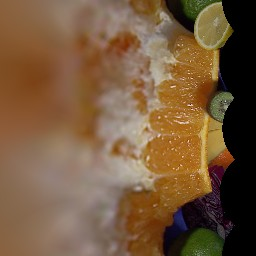
\includegraphics[width=0.4\textwidth]{pics/logpolar.jpg}
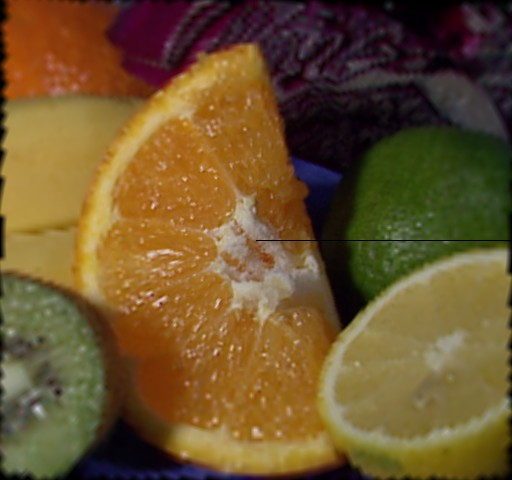
\includegraphics[width=0.4\textwidth]{pics/inv_logpolar.jpg}

\subsection{Morphological Operations}

\cvfunc{CreateStructuringElementEx}\label{CreateStructuringElementEx}

Creates structuring element

\cvexp{
IplConvKernel* cvCreateStructuringElementEx(

int cols,

int rows,

int anchor\_x,

int anchor\_y,

int shape,

int* values=NULL );
}{CPP}{CreateStructuringElementEx(cols,rows,anchor\_x,anchor\_y,shape,values={NULL,0})-> kernel}

\begin{description}
\cvarg{cols}{Number of columns in the structuring element}
\cvarg{rows}{Number of rows in the structuring element}
\cvarg{anchor\_x}{Relative horizontal offset of the anchor point}
\cvarg{anchor\_y}{Relative vertical offset of the anchor point}
\cvarg{shape}{Shape of the structuring element; may have the following values:}
\begin{description}
  \cvarg{CV\_SHAPE\_RECT}{a rectangular element}
  \cvarg{CV\_SHAPE\_CROSS}{a cross-shaped element}
  \cvarg{CV\_SHAPE\_ELLIPSE}{an elliptic element}
  \cvarg{CV\_SHAPE\_CUSTOM}{a user-defined element. In this case the parameter \texttt{values} specifies the mask, that is, which neighbors of the pixel must be considered}
\end{description}
\cvarg{values}{Pointer to the structuring element data, a plane array, representing row-by-row scanning of the element matrix. Non-zero values indicate points that belong to the element. If the pointer is \texttt{NULL}, then all values are considered non-zero, that is, the element is of a rectangular shape. This parameter is considered only if the shape is \texttt{CV\_SHAPE\_CUSTOM} }
\end{description}

The function CreateStructuringElementEx allocates and fills the structure \texttt{IplConvKernel}, which can be used as a structuring element in the morphological operations.

\cvfunc{ReleaseStructuringElement}\label{ReleaseStructuringElement}

Deletes structuring element

\cvexp{
void cvReleaseStructuringElement( IplConvKernel** element );
}{CPP}{PYTHON}

\begin{description}
\cvarg{element}{Pointer to the deleted structuring element}
\end{description}

The function \texttt{cvReleaseStructuringElement} releases the structure \texttt{IplConvKernel} that is no longer needed. If \texttt{*element} is \texttt{NULL}, the function has no effect.

\cvfunc{Erode}\label{Erode}

Erodes image by using arbitrary structuring element

\cvexp{
void cvErode(

const CvArr* src,

CvArr* dst,

IplConvKernel* element=NULL,

int iterations=1 );
}{CPP}{Erode(src,dst,element=NULL,itertions=1)-> None}

\begin{description}
\cvarg{src}{Source image}
\cvarg{dst}{Destination image}
\cvarg{element}{Structuring element used for erosion. If it is \texttt{NULL}, a $3\times 3$ rectangular structuring element is used}
\cvarg{iterations}{Number of times erosion is applied}
\end{description}

The function \texttt{cvErode} erodes the source image using the specified structuring element that determines the shape of a pixel neighborhood over which the minimum is taken:

\[
\min_{(x',y') \, in \, \texttt{element}}src(x+x',y+y')
\]

The function supports the in-place mode. Erosion can be applied several (\texttt{iterations}) times. For color images, each channel is processed independently.

\cvfunc{Dilate}\label{Dilate}

Dilates image by using arbitrary structuring element

\cvexp{
void cvDilate(

const CvArr* src,

CvArr* dst,

IplConvKernel* element=NULL,

int iterations=1 );
}{CPP}{Dilate(src,dst,element=NULL,iterations=1)-> None}

\begin{description}
\cvarg{src}{Source image}
\cvarg{dst}{Destination image}
\cvarg{element}{Structuring element used for dilation. If it is \texttt{NULL}, a $3\times 3$ rectangular structuring element is used}
\cvarg{iterations}{Number of times dilation is applied}
\end{description}

The function \texttt{cvDilate} dilates the source image using the specified structuring element that determines the shape of a pixel neighborhood over which the maximum is taken:

\[
\max_{(x',y') \, in \, \texttt{element}}src(x+x',y+y')
\]

The function supports the in-place mode. Dilation can be applied several (\texttt{iterations}) times. For color images, each channel is processed independently.

\cvfunc{MorphologyEx}\label{MorphologyEx}

Performs advanced morphological transformations

\cvexp{
void cvMorphologyEx(

const CvArr* src,

CvArr* dst,

CvArr* temp,

IplConvKernel* element,

int operation,

int iterations=1 );
}{CPP}{MorphologyEx(src,dst,temp,element,operation,iterations=1)-> None}

\begin{description}
\cvarg{src}{Source image}
\cvarg{dst}{Destination image}
\cvarg{temp}{Temporary image, required in some cases}
\cvarg{element}{Structuring element}
\cvarg{operation}{Type of morphological operation, one of:}
\begin{description}
\cvarg{CV\_MOP\_OPEN}{opening}
\cvarg{CV\_MOP\_CLOSE}{closing}
\cvarg{CV\_MOP\_GRADIENT}{morphological gradient}
\cvarg{CV\_MOP\_TOPHAT}{"top hat"}
\cvarg{CV\_MOP\_BLACKHAT}{"black hat"}
\end{description}
\cvarg{iterations}{Number of times erosion and dilation are applied}
\end{description}

The function \texttt{cvMorphologyEx} can perform advanced morphological transformations using erosion and dilation as basic operations.

Opening:

\[
dst=open(src,element)=dilate(erode(src,element),element)
\]

Closing:

\[
dst=close(src,element)=erode(dilate(src,element),element)
\]

Morphological gradient:

\[
dst=morph\_grad(src,element)=dilate(src,element)-erode(src,element)
\]

"Top hat":

\[
dst=tophat(src,element)=src-open(src,element)
\]

"Black hat":

\[
dst=blackhat(src,element)=close(src,element)-src
\]

The temporary image \texttt{temp} is required for morphological gradient and, in case of in-place operation, for "top hat" and "black hat".

\subsection{Filters and Color Conversion}

\cvfunc{Smooth}\label{Smooth}

Smooths the image in one of several ways

\cvexp{
void cvSmooth(

const CvArr* src,

CvArr* dst,

int smoothtype=CV\_GAUSSIAN,

int param1=3,

int param2=0,

double param3=0, double param4=0 );
}{CPP}{Smooth(src,dst,smoothtype=CV\_GAUSSIAN,param1=3,param2=0,param3=0,param4=0)-> None}

\begin{description}
\cvarg{src}{The source image}
\cvarg{dst}{The destination image}
\cvarg{smoothtype}{Type of the smoothing:
\begin{description}
  \cvarg{CV\_BLUR\_NO\_SCALE (simple blur with no scaling)}{summation over a pixel $\texttt{param1}\times \texttt{param2}$ neighborhood. If the neighborhood size may vary, one may precompute integral image with \cross{Integral} function}
  \cvarg{CV\_BLUR (simple blur)}{summation over a pixel $\texttt{param1}\times \texttt{param2}$ neighborhood with subsequent scaling by $1/(\texttt{param1} \cdot \texttt{param2})$}
  \cvarg{CV\_GAUSSIAN (gaussian blur)}{convolving image with $\texttt{param1}\times \texttt{param2}$ Gaussian kernel}
  \cvarg{CV\_MEDIAN (median blur)}{finding median of $\texttt{param1}\times \texttt{param1}$ neighborhood (i.e. the neighborhood is square)}
  \cvarg{CV\_BILATERAL (bilateral filter)}{applying bilateral $\texttt{param1}\times \texttt{param2}$ filtering with color sigma=\texttt{param3} and space sigma=\texttt{param4}. \texttt{param1} and \texttt{param2} must be equal (square). Information about bilateral filtering can be found at
\url{http://www.dai.ed.ac.uk/CVonline/LOCAL\_COPIES/MANDUCHI1/Bilateral\_Filtering.html}
}
\end{description}}
\cvarg{param1}{The first parameter of smoothing operation}
\cvarg{param2}{The second parameter of smoothing operation. In case of simple scaled/non-scaled and Gaussian blur if \texttt{param2} is zero, it is set to \texttt{param1}}
\cvarg{param3}{In case of Gaussian parameter this parameter may specify Gaussian $\sigma$ (standard deviation). If it is zero, it is calculated from the kernel size:
\[
\sigma = 0.3 (n/2 - 1) + 0.8 \quad \text{where} \quad n=
\begin{array}{l l}
\mbox{\texttt{param1} for horizontal kernel}\\
\mbox{\texttt{param2} for vertical kernel}
\end{array}
\]

Using standard sigma for small kernels ($3\times 3$ to $7\times 7$) gives better speed. If \texttt{param3} is not zero, while \texttt{param1} and \texttt{param2} are zeros, the kernel size is calculated from the sigma (to provide accurate enough operation).}
\end{description}

The function \texttt{cvSmooth} smooths image using one of several methods. Every of the methods has some features and restrictions listed below

Blur with no scaling works with single-channel images only and supports accumulation of 8-bit to 16-bit format (similar to \cross{Sobel} and \cross{Laplace}) and 32-bit floating point to 32-bit floating-point format.

Simple blur and Gaussian blur support 1- or 3-channel, 8-bit and 32-bit floating point images. These two methods can process images in-place.

Median and bilateral filters work with 1- or 3-channel 8-bit images and can not process images in-place.

\cvfunc{Filter2D}\label{Filter2D}

Convolves image with the kernel

\cvexp{
void cvFilter2D(

const CvArr* src,

CvArr* dst,

const CvMat* kernel,

CvPoint anchor=cvPoint(-1,-1));
}{CPP}{Filter2D(src,dst,kernal,anchor=(-1,-1))-> None}

\begin{description}
\cvarg{src}{The source image}
\cvarg{dst}{The destination image}
\cvarg{kernel}{Convolution kernel, single-channel floating point matrix. If you want to apply different kernels to different channels, split the image using cvSplit into separate color planes and process them individually}
\cvarg{anchor}{The anchor of the kernel that indicates the relative position of a filtered point within the kernel. The anchor shoud lie within the kernel. The special default value (-1,-1) means that it is at the kernel center}
\end{description}

The function \texttt{cvFilter2D} applies arbitrary linear filter to the image. In-place operation is supported. When the aperture is partially outside the image, the function interpolates outlier pixel values from the nearest pixels that is inside the image.

\cvfunc{CopyMakeBorder}\label{CopyMakeBorder}

Copies image and makes border around it

\cvexp{
void cvCopyMakeBorder(

const CvArr* src,

CvArr* dst,

CvPoint offset,

int bordertype,

CvScalar value=cvScalarAll(0) );
}{CPP}{CopyMakeBorder(src,dst,offset,bordrtype,value=cvScalarAll(0))-> None}

\begin{description}
\cvarg{src}{The source image}
\cvarg{dst}{The destination image}
\cvarg{offset}{Coordinates of the top-left corner (or bottom-left in case of images with bottom-left origin) of the destination image rectangle where the source image (or its ROI) is copied. Size of the rectanlge matches the source image size/ROI size}
\cvarg{bordertype}{Type of the border to create around the copied source image rectangle:
\begin{description}
\cvarg{IPL\_BORDER\_CONSTANT}{border is filled with the fixed value, passed as last parameter of the function.}
\cvarg{IPL\_BORDER\_REPLICATE}{the pixels from the top and bottom rows, the left-most and right-most columns are replicated to fill the border.}
\end{description}
(The other two border types from IPL, \texttt{IPL\_BORDER\_REFLECT} and \texttt{IPL\_BORDER\_WRAP}, are currently unsupported)}
\cvarg{value}{Value of the border pixels if \texttt{bordertype} is \texttt{IPL\_BORDER\_CONSTANT}}
\end{description}

The function \texttt{cvCopyMakeBorder} copies the source 2D array into interior of destination array and makes a border of the specified type around the copied area. The function is useful when one needs to emulate border type that is different from the one embedded into a specific algorithm implementation. For example, morphological functions, as well as most of other filtering functions in OpenCV, internally use replication border type, while the user may need zero border or a border, filled with 1's or 255's.

\cvfunc{Integral}\label{Integral}

Calculates integral images

\cvexp{
void cvIntegral(

const CvArr* image,

CvArr* sum,

CvArr* sqsum=NULL,

CvArr* tilted\_sum=NULL );
}{CPP}{Integral(image,sum,sqsum=NULL,tilted\_sum=NULL)-> None}

\begin{description}
\cvarg{image}{The source image, $W\times H$, 8-bit or floating-point (32f or 64f) image}
\cvarg{sum}{The integral image, $(W+1)\times (H+1)$, 32-bit integer or double precision floating-point (64f)}
\cvarg{sqsum}{The integral image for squared pixel values, $(W+1)\times (H+1)$, double precision floating-point (64f)}
\cvarg{tilted\_sum}{The integral for the image rotated by 45 degrees, $(W+1)\times (H+1)$, the same data type as \texttt{sum}}
\end{description}

The function \texttt{cvIntegral} calculates one or more integral images for the source image as following:

\[
\texttt{sum}(X,Y) = \sum_{x<X,y<Y} \texttt{image}(x,y)
\]

\[
\texttt{sqsum}(X,Y) = \sum_{x<X,y<Y} \texttt{image}(x,y)^2
\]

\[
\texttt{tilted\_sum}(X,Y) = \sum_{y<Y,abs(x-X)<y} \texttt{image}(x,y)
\]

Using these integral images, one may calculate sum, mean, standard deviation over arbitrary up-right or rotated rectangular region of the image in a constant time, for example:

\[
\sum_{x_1<=x<x_2, \, y_1<=y<y_2} = \texttt{sum}(x_2,y_2)-\texttt{sum}(x_1,y_2)-\texttt{sum}(x_2,y_1)+\texttt{sum}(x_1,x_1)
\]

It makes possible to do a fast blurring or fast block correlation with variable window size etc. In case of multi-channel images sums for each channel are accumulated independently.

\cvfunc{CvtColor}\label{CvtColor}

Converts image from one color space to another

\cvexp{
void cvCvtColor(

const CvArr* src,

CvArr* dst,

int code );
}{CPP}{CvtColor(src,dst,code)-> None}

\begin{description}
\cvarg{src}{The source 8-bit (8u), 16-bit (16u) or single-precision floating-point (32f) image}
\cvarg{dst}{The destination image of the same data type as the source one. The number of channels may be different}
\cvarg{code}{Color conversion operation that can be specifed using \texttt{CV\_ \textit{src\_color\_space} 2 \textit{dst\_color\_space}} constants (see below)}
\end{description}

The function \texttt{cvCvtColor} converts input image from one color
space to another. The function ignores \texttt{colorModel} and
\texttt{channelSeq} fields of \texttt{IplImage} header, so the
source image color space should be specified correctly (including
order of the channels in case of RGB space, e.g. BGR means 24-bit
format with $B_0, G_0, R_0, B_1, G_1, R_1, ...$ layout
whereas RGB means 24-format with $R_0, G_0, B_0, R_1, G_1, B_1, ...$
layout).

The conventional range for R,G,B channel values is:

\begin{itemize}
 \item 0..255 for 8-bit images
 \item 0..65535 for 16-bit images and
 \item 0..1 for floating-point images.
\end{itemize}

Of course, in case of linear transformations the range can be
arbitrary, but in order to get correct results in case of non-linear
transformations, the input image should be scaled if necessary.

The function can do the following transformations:

\begin{itemize}
 \item Transformations within RGB space like adding/removing alpha channel, reversing the channel order, conversion to/from 16-bit RGB color (R5:G6:B5 or R5:G5:B5) color, as well as conversion to/from grayscale using:
 \[
 \text{RGB[A] to Gray:} Y \leftarrow 0.299 \cdot R + 0.587 \cdot G + 0.114 \cdot B
 \]
 and
 \[
 \text{Gray to RGB[A]:} R \leftarrow Y, G \leftarrow Y, B \leftarrow Y, A \leftarrow 0
 \]

The conversion from a RGB image to gray is done with:
\begin{lstlisting}
cvCvtColor(src ,bwsrc, CV_RGB2GRAY)
\end{lstlisting}

 \item RGB $\leftrightarrow$ CIE XYZ.Rec 709 with D65 white point (\texttt{CV\_BGR2XYZ, CV\_RGB2XYZ, CV\_XYZ2BGR, CV\_XYZ2RGB}):
 \[
 \begin{bmatrix}
 X \\
 Y \\
 Z
 \end{bmatrix}
 \leftarrow
 \begin{bmatrix}
0.412453 & 0.357580 & 0.180423\\
0.212671 & 0.715160 & 0.072169\\
0.019334 & 0.119193 & 0.950227
 \end{bmatrix}
 \cdot
 \begin{bmatrix}
 R \\
 G \\
 B
 \end{bmatrix}
 \]
 \[
 \begin{bmatrix}
 R \\
 G \\
 B
 \end{bmatrix}
 \leftarrow
 \begin{bmatrix}
3.240479 & -1.53715 & -0.498535\\
-0.969256 &  1.875991 & 0.041556\\
0.055648 & -0.204043 & 1.057311
 \end{bmatrix}
 \cdot
 \begin{bmatrix}
 X \\
 Y \\
 Z
 \end{bmatrix}
 \]
$X$, $Y$ and $Z$ cover the whole value range (in case of floating-point images $Z$ may exceed 1).

 \item RGB$\leftrightarrow$YCrCb JPEG (a.k.a. YCC) (\texttt{CV\_BGR2YCrCb, CV\_RGB2YCrCb, CV\_YCrCb2BGR, CV\_YCrCb2RGB})
 \[ Y \leftarrow 0.299 \cdot R + 0.587 \cdot G + 0.114 \cdot B \]
 \[  Cr \leftarrow (R-Y) \cdot 0.713 + delta \]
 \[  Cb \leftarrow (B-Y) \cdot 0.564 + delta \]
 \[  R \leftarrow Y + 1.403 \cdot (Cr - delta) \]
 \[  G \leftarrow Y - 0.344 \cdot (Cr - delta) - 0.714 \cdot (Cb - delta) \]
 \[  B \leftarrow Y + 1.773 \cdot (Cb - delta) \]
where
 \[
  delta = \left\{
  \begin{array}{l l}
  128 & \mbox{for 8-bit images}\\
  32768 & \mbox{for 16-bit images}\\
  0.5 & \mbox{for floating-point images}
  \end{array} \right.
 \]
Y, Cr and Cb cover the whole value range.

 \item RGB<=>HSV (\texttt{CV\_BGR2HSV, CV\_RGB2HSV, CV\_HSV2BGR, CV\_HSV2RGB})
  In case of 8-bit and 16-bit images
  R, G and B are converted to floating-point format and scaled to fit 0..1 range
  \[ V \leftarrow max(R,G,B) \]

\[ S \leftarrow \fork{\frac{V-min(R,G,B)}{V}}{if $V \neq 0$}{0}{otherwise} \]
\[ H \leftarrow \forkthree
{{60(G - B)}/{S}}{if $V=R$}
{{120+60(B - R)}/{S}}{if $V=G$}
{{240+60(R - G)}/{S}}{if $V=B$} \]
if $H<0$ then $H \leftarrow H+360$

On output $0 \leq V \leq 1$, $0 \leq S \leq 1$, $0 \leq H \leq 360$.

The values are then converted to the destination data type:
\begin{description}
\item[8-bit images]
\[ V \leftarrow 255 V, S \leftarrow 255 S, H \leftarrow H/2 \text{(to fit to 0...255)} \]
\item[16-bit images (currently not supported)]
\[ V <- 65535 V, S <- 65535 S, H <- H \]
\item[32-bit images]
H, S, V are left as is
\end{description}

 \item RGB $\leftrightarrow$ HLS (\texttt{CV\_BGR2HLS, CV\_RGB2HLS, CV\_HLS2BGR, CV\_HLS2RGB}).
  In case of 8-bit and 16-bit images
  R, G and B are converted to floating-point format and scaled to fit 0..1 range.
  \[ V_{max} \leftarrow {max}(R,G,B) \]
  \[ V_{min} \leftarrow {min}(R,G,B) \]
  \[ L \leftarrow \frac{V_{max} - V_{min}}{2} \]
  \[ S \leftarrow \fork
    {\frac{V_{max} - V_{min}}{V_{max} + V_{min}}}{if $L < 0.5$}
    {\frac{V_{max} - V_{min}}{2 - (V_{max} + V_{min})}}{if $L \ge 0.5$} \]
  \[ H \leftarrow \forkthree
  {{60(G - B)}/{S}}{if $V_{max}=R$}
  {{120+60(B - R)}/{S}}{if $V_{max}=G$}
  {{240+60(R - G)}/{S}}{if $V_{max}=B$} \]
  if $H<0$ then $H \leftarrow H+360$
On output $0 \leq V \leq 1$, $0 \leq S \leq 1$, $0 \leq H \leq 360$.

The values are then converted to the destination data type:
\begin{description}
\item[8-bit images]
\[ V \leftarrow 255 V, S \leftarrow 255 S, H \leftarrow H/2 \text{(to fit to 0...255)} \]
\item[16-bit images (currently not supported)]
\[ V <- 65535 V, S <- 65535 S, H <- H \]
\item[32-bit images]
H, S, V are left as is
\end{description}

 \item RGB $\leftrightarrow$ CIE L*a*b* (\texttt{CV\_BGR2Lab, CV\_RGB2Lab, CV\_Lab2BGR, CV\_Lab2RGB})
  In case of 8-bit and 16-bit images
  R, G and B are converted to floating-point format and scaled to fit 0..1 range
\[ \vecthree{X}{Y}{Z} \leftarrow \vecthreethree
{0.412453}{0.357580}{0.180423}
{0.212671}{0.715160}{0.072169}
{0.019334}{0.119193}{0.950227}
\cdot
\vecthree{R}{G}{B} \]
\[ X \leftarrow X/X_n, \text{where} X_n = 0.950456 \]
\[ Z \leftarrow Z/Z_n, \text{where} Z_n = 1.088754 \]
\[ L \leftarrow \fork
{116*Y^{1/3}-16}{for $Y>0.008856$}
{903.3*Y}{for $Y \le 0.008856$} \]
\[ a \leftarrow 500 (f(X)-f(Y)) + delta \]
\[ b \leftarrow 200 (f(Y)-f(Z)) + delta \]
where
\[f(t)=\fork
{t^{1/3}}{for $t>0.008856$}
{7.787 t+16/116}{for $t<=0.008856$} \]
and
\[ delta = \fork{128}{for 8-bit images}{0}{for floating-point images} \]
On output $0 \leq L \leq 100$, $-127 \leq a \leq 127$, $-127 \leq b \leq 127$

The values are then converted to the destination data type:
\begin{description}
\item[8-bit images]
\[L \leftarrow L*255/100, a \leftarrow a + 128, b \leftarrow b + 128\]
\item[16-bit images] currently not supported
\item[32-bit images]
L, a, b are left as is
\end{description}

 \item RGB $\leftrightarrow$ CIE L*u*v* (\texttt{CV\_BGR2Luv, CV\_RGB2Luv, CV\_Luv2BGR, CV\_Luv2RGB})
  In case of 8-bit and 16-bit images
  R, G and B are converted to floating-point format and scaled to fit 0..1 range
  \[ \vecthree{X}{Y}{Z} \leftarrow \vecthreethree
{0.412453}{0.357580}{0.180423}
{0.212671}{0.715160}{0.072169}
{0.019334}{0.119193}{0.950227}
\cdot
\vecthree{R}{G}{B} \]
\[ L \leftarrow \fork
{116 Y^{1/3}}{for $Y>0.008856$}
{903.3 Y}{for $Y<=0.008856$} \]
\[ u' \leftarrow 4*X/(X + 15*Y + 3 Z) \]
\[ v' \leftarrow 9*Y/(X + 15*Y + 3 Z) \]
\[ u \leftarrow 13*L*(u' - u_n) \quad \text{where} \quad u_n=0.19793943 \]
\[ v \leftarrow 13*L*(v' - v_n) \quad \text{where} \quad v_n=0.46831096 \]
On output $0 \leq L \leq 100$, $-134 \leq u \leq 220$, $-140 \leq v \leq 122$.

The values are then converted to the destination data type:
\begin{description}
\item[8-bit images]
\[L \leftarrow 255/100 L, u \leftarrow 255/354 (u + 134), v \leftarrow 255/256 (v + 140) \]
\item[16-bit images] currently not supported
\item[32-bit images] L, u, v are left as is
\end{description}

The above formulae for converting RGB to/from various color spaces have been taken from multiple sources on Web, primarily from
Ford98
document at Charles Poynton site.

 \item Bayer $\rightarrow$ RGB (\texttt{CV\_BayerBG2BGR, CV\_BayerGB2BGR, CV\_BayerRG2BGR, CV\_BayerGR2BGR, CV\_BayerBG2RGB, CV\_BayerGB2RGB, CV\_BayerRG2RGB, CV\_BayerGR2RGB}) Bayer pattern is widely used in CCD and CMOS cameras. It allows to get color picture out of a single plane where R,G and B pixels (sensors of a particular component) are interleaved like this:

\newcommand{\R}{\color{red}R}
\newcommand{\G}{\color{green}G}
\newcommand{\B}{\color{blue}B}


\[
\definecolor{BackGray}{rgb}{0.8,0.8,0.8}
\begin{array}{ c c c c c }
\R&\G&\R&\G&\R\\
\G&\colorbox{BackGray}{\B}&\colorbox{BackGray}{\G}&\B&\G\\
\R&\G&\R&\G&\R\\
\G&\B&\G&\B&\G\\
\R&\G&\R&\G&\R
\end{array}
\]

The output RGB components of a pixel are interpolated from 1, 2 or
4 neighbors of the pixel having the same color. There are several
modifications of the above pattern that can be achieved by shifting
the pattern one pixel left and/or one pixel up. The two letters
$C_1$ and $C_2$
in the conversion constants
\texttt{CV\_Bayer} $ C_1 C_2 $ \texttt{2BGR}
and
\texttt{CV\_Bayer} $ C_1 C_2 $ \texttt{2RGB}
indicate the particular pattern
type - these are components from the second row, second and third
columns, respectively. For example, the above pattern has very
popular "BG" type.
\end{itemize}

\cvfunc{Threshold}\label{Threshold}

Applies fixed-level threshold to array elements

\cvexp{
double cvThreshold(

const CvArr* src,

CvArr* dst,

double threshold,

double max\_value,

int threshold\_type );
}{CPP}{Threshold(src,dst,threshld,max\_value,threshold\_type)-> None}

\begin{description}
\cvarg{src}{Source array (single-channel, 8-bit of 32-bit floating point)}
\cvarg{dst}{Destination array; must be either the same type as \texttt{src} or 8-bit}
\cvarg{threshold}{Threshold value}
\cvarg{max\_value}{Maximum value to use with \texttt{CV\_THRESH\_BINARY} and \texttt{CV\_THRESH\_BINARY\_INV} thresholding types}
\cvarg{threshold\_type}{Thresholding type (see the discussion)}
\end{description}

The function \texttt{cvThreshold} applies fixed-level thresholding
to single-channel array. The function is typically used to get
bi-level (binary) image out of grayscale image (\cross{CmpS} could
be also used for this purpose) or for removing a noise, i.e. filtering
out pixels with too small or too large values. There are several
types of thresholding the function supports that are determined by
\texttt{threshold\_type}:

\begin{description}
\cvarg{CV\_THRESH\_BINARY}{\[ \texttt{dst}(x,y) = \fork{\texttt{max\_value}}{if $\texttt{src}(x,y) > \texttt{threshold}$}{0}{otherwise} \]}
\cvarg{CV\_THRESH\_BINARY\_INV}{\[ \texttt{dst}(x,y) = \fork{0}{if $\texttt{src}(x,y) > \texttt{threshold}$}{\texttt{max\_value}}{otherwise} \]}
\cvarg{CV\_THRESH\_TRUNC}{\[ \texttt{dst}(x,y) = \fork{\texttt{threshold}}{if $\texttt{src}(x,y) > \texttt{threshold}$}{\texttt{src}(x,y)}{otherwise} \]}
\cvarg{CV\_THRESH\_TOZERO}{\[ \texttt{dst}(x,y) = \fork{\texttt{src}(x,y)}{if $\texttt{src}(x,y) > \texttt{threshold}$}{0}{otherwise} \]}
\cvarg{CV\_THRESH\_TOZERO\_INV}{\[ \texttt{dst}(x,y) = \fork{0}{if $\texttt{src}(x,y) > \texttt{threshold}$}{\texttt{src}(x,y)}{otherwise} \]}
\end{description}

Also, the special value \texttt{CV\_THRESH\_OTSU} may be combined with
one of the above values. In this case the function determines the optimal threshold
value using Otsu's algorithm and uses it instead of the specified \texttt{thresh}.
The function returns the computed threshold value.
Currently, Otsu's method is implemented only for 8-bit images.

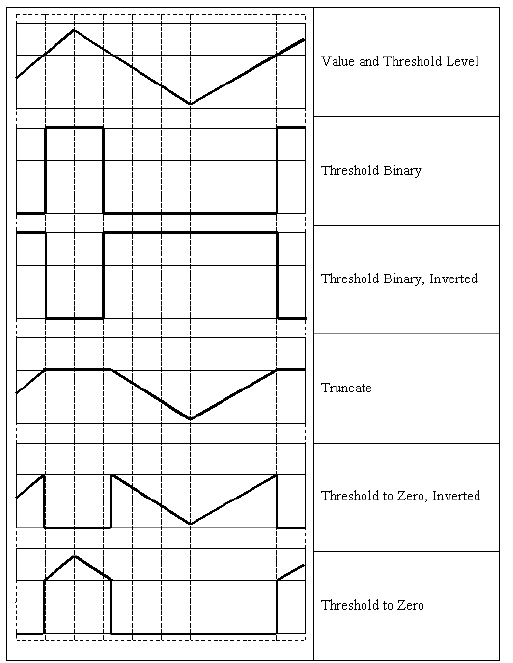
\includegraphics[width=0.5\textwidth]{pics/threshold.png}

\cvfunc{AdaptiveThreshold}\label{AdaptiveThreshold}

Applies adaptive threshold to array

\cvexp{
void cvAdaptiveThreshold(

const CvArr* src,\par CvArr* dst,\par double max\_value,\par
int adaptive\_method=CV\_ADAPTIVE\_THRESH\_MEAN\_C,\par
int threshold\_type=CV\_THRESH\_BINARY,\par
int block\_size=3,\par double param1=5 );

}{CPP}{AdaptiveTheshold(src,dst,max\_value, adaptive\_method=CV\_ADAPTIVE\_THRESH\_MEAN\_C, threshold\_type=CV\_THRESH\_BINARY,block\_size=3,param1=5)-> None}

\begin{description}
\cvarg{src}{Source image}
\cvarg{dst}{Destination image}
\cvarg{max\_value}{Maximum value that is used with \texttt{CV\_THRESH\_BINARY} and \texttt{CV\_THRESH\_BINARY\_INV}}
\cvarg{adaptive\_method}{Adaptive thresholding algorithm to use: \texttt{CV\_ADAPTIVE\_THRESH\_MEAN\_C} or \texttt{CV\_ADAPTIVE\_THRESH\_GAUSSIAN\_C} (see the discussion)}
\cvarg{threshold\_type}{Thresholding type; must be one of
\begin{description}
  \cvarg{CV\_THRESH\_BINARY}{xxx}
  \cvarg{CV\_THRESH\_BINARY\_INV}{xxx}
\end{description}}
\cvarg{block\_size}{The size of a pixel neighborhood that is used to calculate a threshold value for the pixel: 3, 5, 7, ..}
\cvarg{param1}{The method-dependent parameter. For the methods \texttt{CV\_ADAPTIVE\_THRESH\_MEAN\_C} and \texttt{CV\_ADAPTIVE\_THRESH\_GAUSSIAN\_C} it is a constant subtracted from mean or weighted mean (see the discussion), though it may be negative}
\end{description}

The function \texttt{cvAdaptiveThreshold} transforms grayscale image to binary image according to the formulae:

\begin{description}
\cvarg{CV\_THRESH\_BINARY}{\[ dst(x,y) = \fork{\texttt{max\_value}}{if $src(x,y) > T(x,y)$}{0}{otherwise} \]}
\cvarg{CV\_THRESH\_BINARY\_INV}{\[ dst(x,y) = \fork{0}{if $src(x,y) > T(x,y)$}{\texttt{max\_value}}{otherwise} \]}
\end{description}

where $T(x,y)$ is a threshold calculated individually for each pixel.

For the method \texttt{CV\_ADAPTIVE\_THRESH\_MEAN\_C} it is a mean of $\texttt{block\_size} \times \texttt{block\_size}$ pixel neighborhood, subtracted by \texttt{param1}.

For the method \texttt{CV\_ADAPTIVE\_THRESH\_GAUSSIAN\_C} it is a weighted sum (gaussian) of $\texttt{block\_size} \times \texttt{block\_size}$ pixel neighborhood, subtracted by \texttt{param1}.

\subsection{Pyramids and the Applications}

\cvfunc{PyrDown}\label{PyrDown}

Downsamples image

\cvexp{
void cvPyrDown(\par const CvArr* src,\par CvArr* dst,\par int filter=CV\_GAUSSIAN\_5x5 );
}{CPP}{PyrDown(src,dst,filter=CV\_GAUSSIAN\_5X5)-> None}

\begin{description}
\cvarg{src}{The source image}
\cvarg{dst}{The destination image, should have 2x smaller width and height than the source}
\cvarg{filter}{Type of the filter used for convolution; only \texttt{CV\_GAUSSIAN\_5x5} is currently supported}
\end{description}

The function \texttt{cvPyrDown} performs downsampling step of Gaussian pyramid decomposition. First it convolves source image with the specified filter and then downsamples the image by rejecting even rows and columns.

\cvfunc{PyrUp}\label{PyrUp}

Upsamples image

\cvexp{
void cvPyrUp(\par const CvArr* src,\par CvArr* dst,\par int filter=CV\_GAUSSIAN\_5x5 );
}{CPP}{PyrUp(src,dst,filter=CV\_GAUSSIAN\_5X5)-> None}

\begin{description}
\cvarg{src}{The source image}
\cvarg{dst}{The destination image, should have 2x larger width and height than the source}
\cvarg{filter}{Type of the filter used for convolution; only \texttt{CV\_GAUSSIAN\_5x5} is currently supported}
\end{description}

The function \texttt{cvPyrUp} performs up-sampling step of Gaussian pyramid decomposition. First it upsamples the source image by injecting even zero rows and columns and then convolves result with the specified filter multiplied by 4 for interpolation. So the destination image is four times larger than the source image.

\cvfunc{PyrSegmentation}\label{PyrSegmentation}

Implements image segmentation by pyramids

\cvexp{
void cvPyrSegmentation(\par IplImage* src,\par IplImage* dst,\par
                        CvMemStorage* storage,\par CvSeq** comp,\par
                        int level,\par double threshold1,\par double threshold2 );
}{CPP}{PyrSegmentation(src,dst,storage,level,threshold1,threshold2)-> comp}

\begin{description}
\cvarg{src}{The source image}
\cvarg{dst}{The destination image}
\cvarg{storage}{Storage; stores the resulting sequence of connected components}
\cvarg{comp}{Pointer to the output sequence of the segmented components}
\cvarg{level}{Maximum level of the pyramid for the segmentation}
\cvarg{threshold1}{Error threshold for establishing the links}
\cvarg{threshold2}{Error threshold for the segments clustering}
\end{description}

The function \texttt{cvPyrSegmentation} implements image segmentation by pyramids. The pyramid builds up to the level \texttt{level}. The links between any pixel \texttt{a} on level \texttt{i} and its candidate father pixel \texttt{b} on the adjacent level are established if
$p(c(a),c(b))<threshold1$.
After the connected components are defined, they are joined into several clusters.
Any two segments A and B belong to the same cluster, if $p(c(A),c(B))<threshold2$.
The input image has only one channel, then $p(c^1,c^2)=|c^1-c^2|$.
If the input image has three channels (red, green and blue), then
\[
  p(c^1,c^2) = 0.30 (c^1_r - c^2_r) +
               0.59 (c^1_g - c^2_g) +
               0.11 (c^1_b - c^2_b).
\]

There may be more than one connected component per a cluster. The images \texttt{src} and \texttt{dst} should be 8-bit single-channel or 3-channel images or equal size.

\subsection{Connected Components and Contour Retrieval}

\cvstruct{CvConnectedComp}\label{CvConnectedComp}

Connected component

\begin{lstlisting}
    typedef struct CvConnectedComp
    {
        double area;    /* area of the segmented component */
        CvScalar value; /* average color of the connected component */
        CvRect rect;    /* ROI of the segmented component */
        CvSeq* contour; /* optional component boundary
                          (the contour might have child contours corresponding to the holes) */
    } CvConnectedComp;

\end{lstlisting}

\cvfunc{FloodFill}\label{FloodFill}

Fills a connected component with given color

\cvexp{
void cvFloodFill(\par CvArr* image,\par CvPoint seed\_point,\par CvScalar new\_val,\par
                  CvScalar lo\_diff=cvScalarAll(0),\par CvScalar up\_diff=cvScalarAll(0),\par
                  CvConnectedComp* comp=NULL,\par int flags=4,\par CvArr* mask=NULL );

}{CPP}{FloodFill(image,seed\_point,new\_val,lo\_diff=cvScalarAll(0),up\_diff=cvScalarAll(0),flags=4,mask=NULL)-> comp}

\begin{lstlisting}
\#define CV\_FLOODFILL\_FIXED\_RANGE (1 << 16)
\#define CV\_FLOODFILL\_MASK\_ONLY   (1 << 17)
\end{lstlisting}

\begin{description}
\cvarg{image}{Input 1- or 3-channel, 8-bit or floating-point image. It is modified by the function unless \texttt{CV\_FLOODFILL\_MASK\_ONLY} flag is set (see below)}
\cvarg{seed\_point}{The starting point}
\cvarg{new\_val}{New value of repainted domain pixels}
\cvarg{lo\_diff}{Maximal lower brightness/color difference between the currently observed pixel and one of its neighbor belong to the component or seed pixel to add the pixel to component. In case of 8-bit color images it is packed value}
\cvarg{up\_diff}{Maximal upper brightness/color difference between the currently observed pixel and one of its neighbor belong to the component or seed pixel to add the pixel to component. In case of 8-bit color images it is packed value}
\cvarg{comp}{Pointer to structure the function fills with the information about the repainted domain}
\cvarg{flags}{The operation flags. Lower bits contain connectivity value, 4 (by default) or 8, used within the function. Connectivity determines which neighbors of a pixel are considered. Upper bits can be 0 or combination of the following flags:
\begin{description}
  \cvarg{CV\_FLOODFILL\_FIXED\_RANGE}{if set the difference between the current pixel and seed pixel is considered, otherwise difference between neighbor pixels is considered (the range is floating)}
  \cvarg{CV\_FLOODFILL\_MASK\_ONLY}{if set, the function does not fill the image (`new\_val` is ignored), but the fills mask (that must be non-NULL in this case)}
\end{description}}
\cvarg{mask}{Operation mask, should be singe-channel 8-bit image, 2 pixels wider and 2 pixels taller than `image`. If not NULL, the function uses and updates the mask, so user takes responsibility of initializing `mask` content. Floodfilling can't go across non-zero pixels in the mask, for example, an edge detector output can be used as a mask to stop filling at edges. Or it is possible to use the same mask in multiple calls to the function to make sure the filled area do not overlap. ''Note'': because mask is larger than the filled image, pixel in `mask` that corresponds to $(x,y)$ pixel in `image` will have coordinates $(x+1,y+1)$ }
\end{description}

The function \texttt{cvFloodFill} fills a connected component starting from the seed point with the specified color. The connectivity is determined by the closeness of pixel values. The pixel at $(x,y)$ is considered to belong to the repainted domain if:

\begin{description}

\item[grayscale image, floating range] \[
src(x',y')-\texttt{lo\_diff} <= src(x,y) <= src(x',y')+\texttt{up\_diff} \]

\item[grayscale image, fixed range] \[
src(seed.x,seed.y)-\texttt{lo\_diff}<=src(x,y)<=src(seed.x,seed.y)+\texttt{up\_diff} \]

\item[color image, floating range]
\[ src(x',y')_r-\texttt{lo\_diff}_r<=src(x,y)_r<=src(x',y')_r+\texttt{up\_diff}_r \]
\[ src(x',y')_g-\texttt{lo\_diff}_g<=src(x,y)_g<=src(x',y')_g+\texttt{up\_diff}_g \]
\[ src(x',y')_b-\texttt{lo\_diff}_b<=src(x,y)_b<=src(x',y')_b+\texttt{up\_diff}_b \]

\item[color image, fixed range]
\[ src(seed.x,seed.y)_r-\texttt{lo\_diff}_r<=src(x,y)_r<=src(seed.x,seed.y)_r+\texttt{up\_diff}_r \]
\[ src(seed.x,seed.y)_g-\texttt{lo\_diff}_g<=src(x,y)_g<=src(seed.x,seed.y)_g+\texttt{up\_diff}_g \]
\[ src(seed.x,seed.y)_b-\texttt{lo\_diff}_b<=src(x,y)_b<=src(seed.x,seed.y)_b+\texttt{up\_diff}_b \]
\end{description}

where $src(x',y')$ is value of one of pixel neighbors. That is, to be added to the connected component, a pixel's color/brightness should be close enough to:
\begin{itemize}
  \item color/brightness of one of its neighbors that are already referred to the connected component in case of floating range
  \item color/brightness of the seed point in case of fixed range.
\end{itemize}

\cvfunc{FindContours}\label{FindContours}

Finds contours in binary image

\cvexp{
int cvFindContours(\par CvArr* image,\par CvMemStorage* storage,\par CvSeq** first\_contour,\par
                    int header\_size=sizeof(CvContour),\par int mode=CV\_RETR\_LIST,\par
                    int method=CV\_CHAIN\_APPROX\_SIMPLE,\par CvPoint offset=cvPoint(0,\par0) );
}{CPP}{PYTHON}

\begin{description}
\cvarg{image}{The source 8-bit single channel image. Non-zero pixels are treated as 1's, zero pixels remain 0's - that is image treated as `binary`. To get such a binary image from grayscale, one may use \cross{Threshold}, \cross{AdaptiveThreshold} or \cross{Canny}. The function modifies the source image content}
\cvarg{storage}{Container of the retrieved contours}
\cvarg{first\_contour}{Output parameter, will contain the pointer to the first outer contour}
\cvarg{header\_size}{Size of the sequence header, $\ge \texttt{sizeof(CvChain)}$ if $\texttt{method} =\texttt{CV\_CHAIN\_CODE}$,
and $\ge \texttt{sizeof(CvContour)}$ otherwise}
\cvarg{mode}{Retrieval mode
\begin{description}
  \cvarg{CV\_RETR\_EXTERNAL}{retrive only the extreme outer contours}
  \cvarg{CV\_RETR\_LIST}{retrieve all the contours and puts them in the list}
  \cvarg{CV\_RETR\_CCOMP}{retrieve all the contours and organizes them into two-level hierarchy: top level are external boundaries of the components, second level are bounda boundaries of the holes}
  \cvarg{CV\_RETR\_TREE}{retrieve all the contours and reconstructs the full hierarchy of nested contours}
\end{description}}
\cvarg{method}{Approximation method (for all the modes, except \texttt{CV\_LINK\_RUNS}, which uses built-in approximation)
\begin{description}
  \cvarg{CV\_CHAIN\_CODE}{output contours in the Freeman chain code. All other methods output polygons (sequences of vertices).}
  \cvarg{CV\_CHAIN\_APPROX\_NONE}{translate all the points from the chain code into points;}
  \cvarg{CV\_CHAIN\_APPROX\_SIMPLE}{compress horizontal, vertical, and diagonal segments, that is, the function leaves only their ending points;}
  \cvarg{CV\_CHAIN\_APPROX\_TC89\_L1,CV\_CHAIN\_APPROX\_TC89\_KCOS}{apply one of the flavors of Teh-Chin chain approximation algorithm.}
  \cvarg{CV\_LINK\_RUNS}{use completely different contour retrieval algorithm via linking of horizontal segments of 1's. Only \texttt{CV\_RETR\_LIST} retrieval mode can be used with this method.}
\end{description}}
\cvarg{offset}{Offset, by which every contour point is shifted. This is useful if the contours are extracted from the image ROI and then they should be analyzed in the whole image context}
\end{description}

The function \texttt{cvFindContours} retrieves contours from the
binary image and returns the number of retrieved contours. The
pointer \texttt{first\_contour} is filled by the function. It will
contain pointer to the first most outer contour or \texttt{NULL} if no
contours is detected (if the image is completely black). Other
contours may be reached from \texttt{first\_contour} using
\texttt{h\_next} and \texttt{v\_next} links. The sample in
\cross{DrawContours} discussion shows how to use contours for
connected component detection. Contours can be also used for shape
analysis and object recognition - see \texttt{squares.c} in OpenCV
sample directory.

\cvfunc{StartFindContours}\label{StartFindContours}

Initializes contour scanning process

\cvexp{
CvContourScanner cvStartFindContours(\par CvArr* image,\par CvMemStorage* storage,\par
                                      int header\_size=sizeof(CvContour),\par
                                      int mode=CV\_RETR\_LIST,\par
                                      int method=CV\_CHAIN\_APPROX\_SIMPLE,\par
                                      CvPoint offset=cvPoint(0,\par0) );
}{CPP}{PYTHON}

\begin{description}
\cvarg{image}{The source 8-bit single channel binary image}
\cvarg{storage}{Container of the retrieved contours}
\cvarg{header\_size}{Size of the sequence header, >=sizeof(CvChain) if \texttt{method} =CV\_CHAIN\_CODE, and >=sizeof(CvContour) otherwise}
\cvarg{mode}{Retrieval mode; see \cross{FindContours}}
\cvarg{method}{Approximation method. It has the same meaning as in \cross{FindContours}, but \texttt{CV\_LINK\_RUNS} can not be used here}
\cvarg{offset}{ROI offset; see \cross{FindContours}}
\end{description}

The function \texttt{cvStartFindContours} initializes and returns pointer to the contour scanner. The scanner is used further in \cross{FindNextContour} to retrieve the rest of contours.

\cvfunc{FindNextContour}\label{FindNextContour}

Finds next contour in the image

\cvexp{
CvSeq* cvFindNextContour( \par CvContourScanner scanner );
}{CPP}{PYTHON}

\begin{description}
\cvarg{scanner}{Contour scanner initialized by The function \texttt{cvStartFindContours} }
\end{description}

The function \texttt{cvFindNextContour} locates and retrieves the next contour in the image and returns pointer to it. The function returns NULL, if there is no more contours.

\cvfunc{SubstituteContour}\label{SubstituteContour}

Replaces retrieved contour

\cvexp{
void cvSubstituteContour( \par CvContourScanner scanner, \par CvSeq* new\_contour );
}{CPP}{PYTHON}

\begin{description}
\cvarg{scanner}{Contour scanner initialized by \cross{StartFindContours} }
\cvarg{new\_contour}{Substituting contour}
\end{description}

The function \texttt{cvSubstituteContour} replaces the retrieved
contour, that was returned from the preceding call of The function
\cross{FindNextContour} and stored inside the contour scanner
state, with the user-specified contour. The contour is inserted
into the resulting structure, list, two-level hierarchy, or tree,
depending on the retrieval mode. If the parameter \texttt{new\_contour}
is \texttt{NULL}, the retrieved contour is not included into the
resulting structure, nor all of its children that might be added
to this structure later.

\cvfunc{EndFindContours}\label{EndFindContours}

Finishes scanning process

\cvexp{
CvSeq* cvEndFindContours( \par CvContourScanner* scanner );
}{CPP}{PYTHON}

\begin{description}
\cvarg{scanner}{Pointer to the contour scanner}
\end{description}

The function \texttt{cvEndFindContours} finishes the scanning process and returns the pointer to the first contour on the highest level.

\cvfunc{PyrMeanShiftFiltering}

Does meanshift image segmentation

\cvexp{

void cvPyrMeanShiftFiltering( \par const CvArr* src, \par CvArr* dst,
     \par double sp, \par double sr, \par int max\_level=1,
     \par CvTermCriteria termcrit=\par cvTermCriteria(CV\_TERMCRIT\_ITER+CV\_TERMCRIT\_EPS,5,1));

}{CPP}{PyrMeanShiftFiltering(src,dst,sp,sr,max\_level=1,
       termcrit=\par cvTermCriteria(CV\_TERMCRIT\_ITER+CV\_TERMCRIT\_EPS,5,1))-> None}

\begin{description}
\cvarg{src}{The source 8-bit, 3-channel image.}
\cvarg{dst}{The destination image of the same format and the same size as the source.}
\cvarg{sp}{The spatial window radius.}
\cvarg{sr}{The color window radius.}
\cvarg{max\_level}{Maximum level of the pyramid for the segmentation.}
\cvarg{termcrit}{Termination criteria: when to stop meanshift iterations.}
\end{description}

The function \texttt{cvPyrMeanShiftFiltering} implements the filtering stage of meanshift segmentation, that is, the output of the function is the filtered "posterized" image with color gradients and fine-grain texture flattened. At every pixel $(X,Y)$ of the input image (or down-sized input image, see below) the function executes meanshift iterations, that is, the pixel $(X,Y)$ neighborhood in the joint space-color hyperspace is considered: 

{$(x,y): X-sp≤x≤X+sp \&\& Y-sp≤y≤Y+sp \&\& ||(R,G,B)-(r,g,b)|| ≤ sr$},

where \texttt{(R,G,B)} and \texttt{(r,g,b)} are the vectors of color components at \texttt{(X,Y)} and \texttt{(x,y)}, respectively (though, the algorithm does not depend on the color space used, so any 3-component color space can be used instead). Over the neighborhood the average spatial value \texttt{(X',Y')} and average color vector \texttt{(R',G',B')} are found and they act as the neighborhood center on the next iteration: 

$(X,Y)~(X',Y'), (R,G,B)~(R',G',B').$

After the iterations over, the color components of the initial pixel (that is, the pixel from where the iterations started) are set to the final value (average color at the last iteration): 

$I(X,Y) <- (R*,G*,B*).$

Then \texttt{max\_level}$>$0, the gaussian pyramid of \texttt{max\_level}+1 levels is built, and the above procedure is run on the smallest layer. After that, the results are propagated to the larger layer and the iterations are run again only on those pixels where the layer colors differ much ($>$\texttt{sr}) from the lower-resolution layer, that is, the boundaries of the color regions are clarified. Note, that the results will be actually different from the ones obtained by running the meanshift procedure on the whole original image (i.e. when \texttt{max\_level}==0).


\cvfunc{Watershed}

Does watershed segmentation.

\cvexp{

void cvWatershed( const CvArr* image, CvArr* markers );


}{CPP}{Watershed(image,markers)-> None}

\begin{description}
\cvarg{image}{The input 8-bit 3-channel image.} 
\cvarg{markers}{The input/output 32-bit single-channel image (map) of markers.}
\end{description}

The function \texttt{cvWatershed} implements one of the variants of watershed, non-parametric marker-based segmentation algorithm, described in \href{#Meyer92}{[Meyer92]} Before passing the image to the function, user has to outline roughly the desired regions in the image \texttt{markers} with positive ($>$0) indices, i.e. every region is represented as one or more connected components with the pixel values 1, 2, 3 etc. Those components will be "seeds" of the future image regions. All the other pixels in \texttt{markers}, which relation to the outlined regions is not known and should be defined by the algorithm, should be set to 0's. On the output of the function, each pixel in markers is set to one of values of the "seed" components, or to -1 at boundaries between the regions.

Note, that it is not necessary that every two neighbor connected components are separated by a watershed boundary (-1's pixels), for example, in case when such tangent components exist in the initial marker image. Visual demonstration and usage example of the function can be found in OpenCV samples directory; see \texttt{watershed.cpp} demo.

\subsection{Image and Contour moments}

\cvfunc{Moments}\label{Moments}

Calculates all moments up to third order of a polygon or rasterized shape

\cvexp{
void cvMoments( \par const CvArr* arr,\par CvMoments* moments,\par int binary=0 );
}{CPP}{PYTHON}

\begin{description}
\cvarg{arr}{Image (1-channel or 3-channel with COI set) or polygon (CvSeq of points or a vector of points)}
\cvarg{moments}{Pointer to returned moment state structure}
\cvarg{binary}{(For images only) If the flag is non-zero, all the zero pixel values are treated as zeroes, all the others are treated as 1's}
\end{description}

The function \texttt{cvMoments} calculates spatial and central moments up to the third order and writes them to \texttt{moments}. The moments may be used then to calculate gravity center of the shape, its area, main axises and various shape characeteristics including 7 Hu invariants.

\cvfunc{GetSpatialMoment}\label{GetSpatialMoment}

Retrieves spatial moment from moment state structure

\cvexp{
double cvGetSpatialMoment( \par CvMoments* moments, \par int x\_order, \par int y\_order );
}{CPP}{PYTHON}

\begin{description}
\cvarg{moments}{The moment state, calculated by \cross{Moments}}
\cvarg{x\_order}{x order of the retrieved moment, $\texttt{x\_order} >= 0$}
\cvarg{y\_order}{y order of the retrieved moment, $\texttt{y\_order} >= 0$ and $\texttt{x\_order} + \texttt{y\_order} <= 3$}
\end{description}

The function \texttt{cvGetSpatialMoment} retrieves the spatial moment, which in case of image moments is defined as:

\[
M_{x\_order, \, y\_order} = \sum_{x,y} (I(x,y) \cdot x^{x\_order} \cdot y^{y\_order})
\]

where $I(x,y)$ is the intensity of the pixel $(x, y)$.

\cvfunc{GetCentralMoment}\label{GetCentralMoment}

Retrieves central moment from moment state structure

\cvexp{
double cvGetCentralMoment( \par CvMoments* moments,\par int x\_order,\par int y\_order );
}{CPP}{PYTHON}

\begin{description}
\cvarg{moments}{Pointer to the moment state structure}
\cvarg{x\_order}{x order of the retrieved moment, $\texttt{x\_order} >= 0$}
\cvarg{y\_order}{y order of the retrieved moment, $\texttt{y\_order} >= 0$ and $\texttt{x\_order} + \texttt{y\_order} <= 3$}
\end{description}

The function \texttt{cvGetCentralMoment} retrieves the central moment, which in case of image moments is defined as:

\[
\mu_{x\_order, \, y\_order} = \sum_{x,y} (I(x,y) \cdot (x-x_c)^{x\_order} \cdot (y-y_c)^{y\_order})
\]

where $x_c,y_c$ are coordinates of the gravity center:

\[
x_c=\frac{M_{10}}{M_{00}}, y_c=\frac{M_{01}}{M_{00}}
\]

\cvfunc{GetNormalizedCentralMoment}\label{GetNormalizedCentralMoment}

Retrieves normalized central moment from moment state structure

\cvexp{
double cvGetNormalizedCentralMoment( \par CvMoments* moments,\par int x\_order,\par int y\_order );
}{CPP}{PYTHON}

\begin{description}
\cvarg{moments}{Pointer to the moment state structure}
\cvarg{x\_order}{x order of the retrieved moment, $\texttt{x\_order} >= 0$}
\cvarg{y\_order}{y order of the retrieved moment, $\texttt{y\_order} >= 0$ and $\texttt{x\_order} + \texttt{y\_order} <= 3$}
\end{description}

The function \texttt{cvGetNormalizedCentralMoment} retrieves the normalized central moment:

\[
\eta_{x\_order, \, y\_order} = \frac{\mu_{x\_order, \, y\_order}}{M_{00}^{(y\_order+x\_order)/2+1}}
\]

\cvfunc{GetHuMoments}\label{GetHuMoments}

Calculates seven Hu invariants

\cvexp{
void cvGetHuMoments( CvMoments* moments, CvHuMoments* hu\_moments );
}{CPP}{PYTHON}

\begin{description}
\cvarg{moments}{Pointer to the moment state structure}
\cvarg{hu\_moments}{Pointer to Hu moments structure}
\end{description}

The function \texttt{cvGetHuMoments} calculates seven Hu invariants that are defined as:

\[ \begin{array}{l}
h1=\eta_{20}+\eta_{02}\\
h2=(\eta_{20}-\eta_{02})^{2}+4\eta_{11}^{2}\\
h1=\eta_{20}+\eta_{02}\\
h2=(\eta_{20}-\eta_{02})^{2}+4\eta_{11}^{2}\\
h3=(\eta_{30}-3\eta_{12})^{2}+ (3\eta_{21}-\eta_{03})^{2}\\
h4=(\eta_{30}+\eta_{12})^{2}+ (\eta_{21}+\eta_{03})^{2}\\
h5=(\eta_{30}-3\eta_{12})(\eta_{30}+\eta_{12})[(\eta_{30}+\eta_{12})^{2}-3(\eta_{21}+\eta_{03})^{2}]+(3\eta_{21}-\eta_{03})(\eta_{21}+\eta_{03})[3(\eta_{30}+\eta_{12})^{2}-(\eta_{21}+\eta_{03})^{2}]\\
h6=(\eta_{20}-\eta_{02})[(\eta_{30}+\eta_{12})^{2}- (\eta_{21}+\eta_{03})^{2}]+4\eta_{11}(\eta_{30}+\eta_{12})(\eta_{21}+\eta_{03})\\
h7=(3\eta_{21}-\eta_{03})(\eta_{21}+\eta_{03})[3(\eta_{30}+\eta_{12})^{2}-(\eta_{21}+\eta_{03})^{2}]-(\eta_{30}-3\eta_{12})(\eta_{21}+\eta_{03})[3(\eta_{30}+\eta_{12})^{2}-(\eta_{21}+\eta_{03})^{2}]\\
\end{array}
\]

where $\eta_{i,j}$ are normalized central moments of $2^{nd}$ and $3^{rd}$ orders. 
These values are proved to be invariants to the image scale, rotation, and reflection except the seventh one, whose sign is changed by reflection.

\subsection{Special Image Transforms}

\cvfunc{HoughLines2}\label{HoughLines2}

Finds lines in binary image using Hough transform

\cvexp{
CvSeq* cvHoughLines2( \par CvArr* image,\par void* line\_storage,\par int method,\par double rho,\par double theta,\par int threshold,\par double param1=0,\par double param2=0 );
}{CPP}{HoughLines2(image,storage,method,rho,theta,threshold,param1=0,parma2=0)-> lines}

\begin{description}
\cvarg{image}{The input 8-bit single-channel binary image. In case of probabilistic method the image is modified by the function}
\cvarg{line\_storage}{The storage for the lines detected. It can
be a memory storage (in this case a sequence of lines is created in
the storage and returned by the function) or single row/single column
matrix (CvMat*) of a particular type (see below) to which the lines'
parameters are written. The matrix header is modified by the function
so its \texttt{cols} or \texttt{rows} will contain a number of lines
detected. If \texttt{line\_storage} is a matrix and the actual number
of lines exceeds the matrix size, the maximum possible number of lines
is returned (in case of standard hough transform the lines are sorted
by the accumulator value)}
\cvarg{method}{The Hough transform variant, one of:
\begin{description}
  \cvarg{CV\_HOUGH\_STANDARD}{classical or standard Hough transform. Every line is represented by two floating-point numbers $(\rho, \theta)$, where $\rho$ is a distance between (0,0) point and the line, and $\theta$ is the angle between x-axis and the normal to the line. Thus, the matrix must be (the created sequence will be) of \texttt{CV\_32FC2} type.}
  \cvarg{CV\_HOUGH\_PROBABILISTIC}{probabilistic Hough transform (more efficient in case if picture contains a few long linear segments). It returns line segments rather than the whole lines. Every segment is represented by starting and ending points, and the matrix must be (the created sequence will be) of \texttt{CV\_32SC4} type.}
  \cvarg{CV\_HOUGH\_MULTI\_SCALE}{multi-scale variant of classical Hough transform. The lines are encoded the same way as in \texttt{CV\_HOUGH\_STANDARD}.}
\end{description}}
\cvarg{rho}{Distance resolution in pixel-related units}
\cvarg{theta}{Angle resolution measured in radians}
\cvarg{threshold}{Threshold parameter. A line is returned by the function if the corresponding accumulator value is greater than \texttt{threshold}}
\cvarg{param1}{The first method-dependent parameter:
\begin{itemize}
  \item For classical Hough transform it is not used (0).
  \item For probabilistic Hough transform it is the minimum line length.
  \item For multi-scale Hough transform it is divisor for distance resolution $\rho$. (The coarse distance resolution will be $\rho$ and the accurate resolution will be $(\rho / \texttt{param1})$).
\end{itemize}}
\cvarg{param2}{The second method-dependent parameter:
\begin{itemize}
  \item For classical Hough transform it is not used (0).
  \item For probabilistic Hough transform it is the maximum gap between line segments lieing on the same line to treat them as the single line segment (i.e. to join them).
  \item For multi-scale Hough transform it is divisor for angle resolution $\theta$. (The coarse angle resolution will be $\theta$ and the accurate resolution will be $(\theta / \texttt{param2})$).
\end{itemize}}
\end{description}

The function \texttt{cvHoughLines2} implements a few variants of Hough transform for line detection.

% ===== Example. Detecting lines with Hough transform. =====
\begin{lstlisting}
/* This is a standalone program. Pass an image name as a first parameter
of the program.  Switch between standard and probabilistic Hough transform
by changing "#if 1" to "#if 0" and back */
#include <cv.h>
#include <highgui.h>
#include <math.h>

int main(int argc, char** argv)
{
    IplImage* src;
    if( argc == 2 && (src=cvLoadImage(argv[1], 0))!= 0)
    {
        IplImage* dst = cvCreateImage( cvGetSize(src), 8, 1 );
        IplImage* color_dst = cvCreateImage( cvGetSize(src), 8, 3 );
        CvMemStorage* storage = cvCreateMemStorage(0);
        CvSeq* lines = 0;
        int i;
        cvCanny( src, dst, 50, 200, 3 );
        cvCvtColor( dst, color_dst, CV_GRAY2BGR );
#if 1
        lines = cvHoughLines2( dst,
                               storage,
                               CV_HOUGH_STANDARD,
                               1,
                               CV_PI/180,
                               100,
                               0,
                               0 );

        for( i = 0; i < MIN(lines->total,100); i++ )
        {
            float* line = (float*)cvGetSeqElem(lines,i);
            float rho = line[0];
            float theta = line[1];
            CvPoint pt1, pt2;
            double a = cos(theta), b = sin(theta);
            double x0 = a*rho, y0 = b*rho;
            pt1.x = cvRound(x0 + 1000*(-b));
            pt1.y = cvRound(y0 + 1000*(a));
            pt2.x = cvRound(x0 - 1000*(-b));
            pt2.y = cvRound(y0 - 1000*(a));
            cvLine( color_dst, pt1, pt2, CV_RGB(255,0,0), 3, 8 );
        }
#else
        lines = cvHoughLines2( dst,
                               storage,
                               CV_HOUGH_PROBABILISTIC,
                               1,
                               CV_PI/180,
                               80,
                               30,
                               10 );
        for( i = 0; i < lines->total; i++ )
        {
            CvPoint* line = (CvPoint*)cvGetSeqElem(lines,i);
            cvLine( color_dst, line[0], line[1], CV_RGB(255,0,0), 3, 8 );
        }
#endif
        cvNamedWindow( "Source", 1 );
        cvShowImage( "Source", src );

        cvNamedWindow( "Hough", 1 );
        cvShowImage( "Hough", color_dst );

        cvWaitKey(0);
    }
}
\end{lstlisting}

This is the sample picture the function parameters have been tuned for:

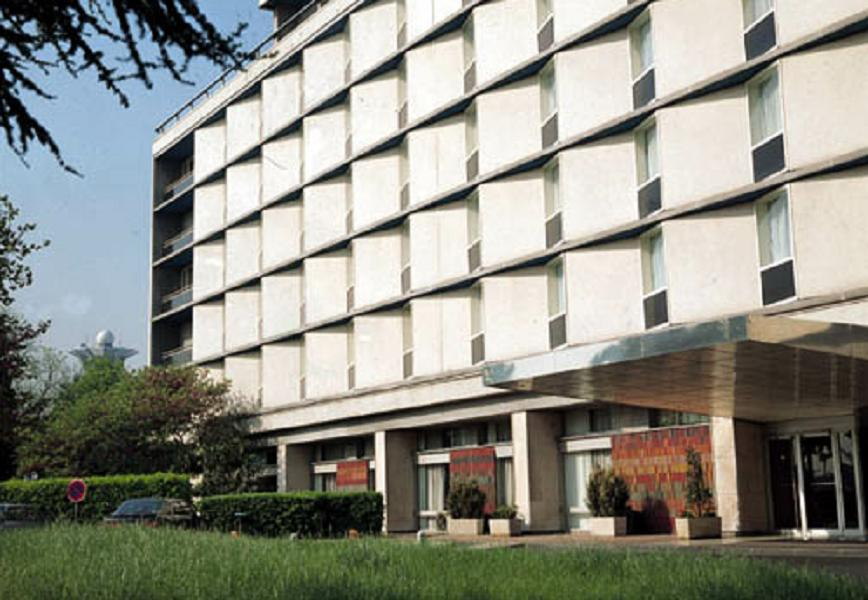
\includegraphics[width=0.5\textwidth]{pics/building.jpg}

And this is the output of the above program in case of probabilistic Hough transform (\texttt{\#if 0} case):

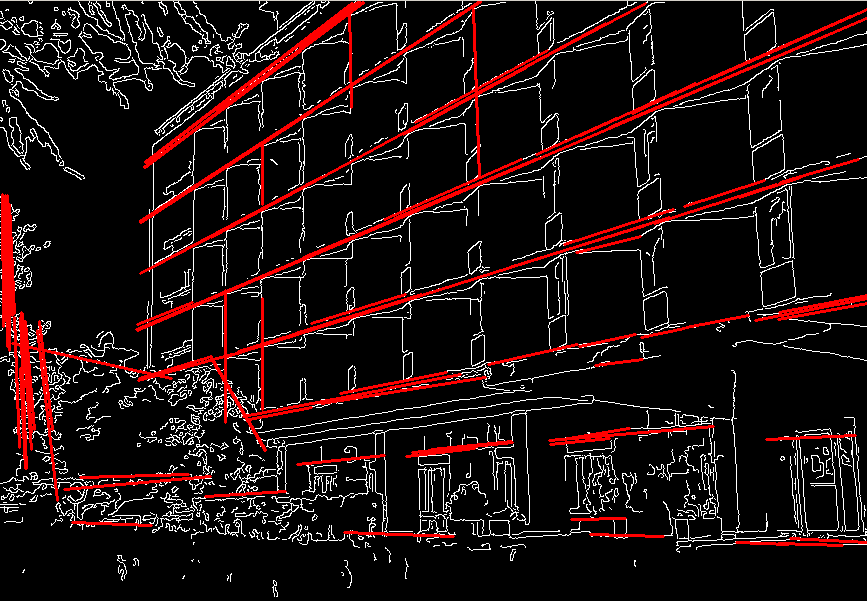
\includegraphics[width=0.5\textwidth]{pics/houghp.png}

\cvfunc{HoughCircles}\label{HoughCircles}

Finds circles in grayscale image using Hough transform

\cvexp{
CvSeq* cvHoughCircles( \par CvArr* image,\par void* circle\_storage,\par int method,\par double dp,\par double min\_dist,\par double param1=100,\par double param2=100,\par int min\_radius=0,\par int max\_radius=0 );
}{CPP}{HoughCircles(image,circle\_storage,method,dp,min\_dist,param1=100,param2=100,min\_radius=0,max\_radius=0)-> None}

\begin{description}
\cvarg{image}{The input 8-bit single-channel grayscale image}
\cvarg{circle\_storage}{The storage for the circles detected. It can be a memory storage (in this case a sequence of circles is created in the storage and returned by the function) or single row/single column matrix (CvMat*) of type \texttt{CV\_32FC3}, to which the circles' parameters are written. The matrix header is modified by the function so its \texttt{cols} or \texttt{rows} will contain a number of lines detected. If \texttt{circle\_storage} is a matrix and the actual number of lines exceeds the matrix size, the maximum possible number of circles is returned. Every circle is encoded as 3 floating-point numbers: center coordinates (x,y) and the radius}
\cvarg{method}{Currently, the only implemented method is \texttt{CV\_HOUGH\_GRADIENT}, which is basically 21HT, described in Yuen03.}
\cvarg{dp}{Resolution of the accumulator used to detect centers of the circles. For example, if it is 1, the accumulator will have the same resolution as the input image, if it is 2 - accumulator will have twice smaller width and height, etc}
\cvarg{min\_dist}{Minimum distance between centers of the detected circles. If the parameter is too small, multiple neighbor circles may be falsely detected in addition to a true one. If it is too large, some circles may be missed}
\cvarg{param1}{The first method-specific parameter. In case of \texttt{CV\_HOUGH\_GRADIENT} it is the higher threshold of the two passed to \cross{Canny} edge detector (the lower one will be twice smaller)}
\cvarg{param2}{The second method-specific parameter. In case of \texttt{CV\_HOUGH\_GRADIENT} it is accumulator threshold at the center detection stage. The smaller it is, the more false circles may be detected. Circles, corresponding to the larger accumulator values, will be returned first}
\cvarg{min\_radius}{Minimum circle radius}
\cvarg{max\_radius}{Maximum circle radius}
\end{description}

The function \texttt{cvHoughCircles} finds circles in grayscale image using some modification of Hough transform.

% ===== Example. Detecting circles with Hough transform. =====
\begin{lstlisting}
#include <cv.h>
#include <highgui.h>
#include <math.h>

int main(int argc, char** argv)
{
    IplImage* img;
    if( argc == 2 && (img=cvLoadImage(argv[1], 1))!= 0)
    {
        IplImage* gray = cvCreateImage( cvGetSize(img), 8, 1 );
        CvMemStorage* storage = cvCreateMemStorage(0);
        cvCvtColor( img, gray, CV_BGR2GRAY );
        // smooth it, otherwise a lot of false circles may be detected
        cvSmooth( gray, gray, CV_GAUSSIAN, 9, 9 );
        CvSeq* circles = cvHoughCircles( gray,
                                         storage,
                                         CV_HOUGH_GRADIENT,
                                         2,
                                         gray->height/4,
                                         200,
                                         100 );
        int i;
        for( i = 0; i < circles->total; i++ )
        {
             float* p = (float*)cvGetSeqElem( circles, i );
             cvCircle( img,
                       cvPoint(cvRound(p[0]),cvRound(p[1])),
                       3,
                       CV_RGB(0,255,0),
                       -1, 8, 0 );
             cvCircle( img,
                       cvPoint(cvRound(p[0]),cvRound(p[1])),
                       cvRound(p[2]),
                       CV_RGB(255,0,0),
                       3, 8, 0 );
        }
        cvNamedWindow( "circles", 1 );
        cvShowImage( "circles", img );
    }
    return 0;
}
\end{lstlisting}

\cvfunc{DistTransform}\label{DistTransform}

Calculates distance to closest zero pixel for all non-zero pixels of source image

\cvexp{
void cvDistTransform( \par const CvArr* src,\par CvArr* dst,\par int distance\_type=CV\_DIST\_L2,\par int mask\_size=3,\par const float* mask=NULL,\par CvArr* labels=NULL );
}{CPP}{DistTransform(src,dst,distance\_type=CV\_DIST\_L2,mask\_size=3,mask={NULL,0},labels=NULL)-> None}

\begin{description}
\cvarg{src}{Source 8-bit single-channel (binary) image}
\cvarg{dst}{Output image with calculated distances (32-bit floating-point, single-channel)}
\cvarg{distance\_type}{Type of distance; can be \texttt{CV\_DIST\_L1, CV\_DIST\_L2, CV\_DIST\_C} or \texttt{CV\_DIST\_USER}}
\cvarg{mask\_size}{Size of distance transform mask; can be 3 or 5. In case of \texttt{CV\_DIST\_L1} or \texttt{CV\_DIST\_C} the parameter is forced to 3, because $3\times 3$ mask gives the same result as $5\times 5 $ yet it is faster}
\cvarg{mask}{User-defined mask in case of user-defined distance, it consists of 2 numbers (horizontal/vertical shift cost, diagonal shift cost) in case of $3\times 3$ mask and 3 numbers (horizontal/vertical shift cost, diagonal shift cost, knight's move cost) in case of $5\times 5$ mask}
\cvarg{labels}{The optional output 2d array of labels of integer type and the same size as \texttt{src} and \texttt{dst}}
\end{description}

The function \texttt{cvDistTransform} calculates the approximated
distance from every binary image pixel to the nearest zero pixel.
For zero pixels the function sets the zero distance, for others it
finds the shortest path consisting of basic shifts: horizontal,
vertical, diagonal or knight's move (the latest is available for
$5\times 5$ mask). The overal distance is calculated as a sum of these
basic distances. Because the distance function should be symmetric,
all the horizontal and vertical shifts must have the same cost (that
is denoted as \texttt{a}), all the diagonal shifts must have the
same cost (denoted \texttt{b}), and all knight?s moves must have
the same cost (denoted \texttt{c}). For \texttt{CV\_DIST\_C} and
\texttt{CV\_DIST\_L1} types the distance is calculated precisely,
whereas for \texttt{CV\_DIST\_L2} (Euclidian distance) the distance
can be calculated only with some relative error ($5\times 5$ mask
gives more accurate results), OpenCV uses the values suggested in
\cite{Borgefors86}:


\begin{tabular}{| c | c | c |}
\hline
\texttt{CV\_DIST\_C}  & $(3\times 3)$ & a = 1, b = 1\\ \hline
\texttt{CV\_DIST\_L1} & $(3\times 3)$ & a = 1, b = 2\\ \hline
\texttt{CV\_DIST\_L2} & $(3\times 3)$ & a=0.955, b=1.3693\\ \hline
\texttt{CV\_DIST\_L2} & $(5\times 5)$ & a=1, b=1.4, c=2.1969\\ \hline
\end{tabular}

And below are samples of distance field (black (0) pixel is in the middle of white square) in case of user-defined distance:

User-defined $3 \times 3$ mask (a=1, b=1.5)

\begin{tabular}{| c | c | c | c | c | c | c |}
\hline
4.5 & 4 & 3.5 & 3 & 3.5 & 4 & 4.5\\ \hline
4 & 3 & 2.5 & 2 & 2.5 & 3 & 4\\ \hline
3.5 & 2.5 & 1.5 & 1 & 1.5 & 2.5 & 3.5\\ \hline
3 & 2 & 1 &     & 1 & 2 & 3\\ \hline
3.5 & 2.5 & 1.5 & 1 & 1.5 & 2.5 & 3.5\\ \hline
4 & 3 & 2.5 & 2 & 2.5 & 3 & 4\\ \hline
4.5 & 4 & 3.5 & 3 & 3.5 & 4 & 4.5\\ \hline
\end{tabular}

User-defined $5 \times 5$ mask (a=1, b=1.5, c=2)

\begin{tabular}{| c | c | c | c | c | c | c |}
\hline
4.5 & 3.5 & 3 & 3 & 3 & 3.5 & 4.5\\ \hline
3.5 & 3 & 2 & 2 & 2 & 3 & 3.5\\ \hline
3 & 2 & 1.5 & 1 & 1.5 & 2 & 3\\ \hline
3 & 2 & 1 & & 1 & 2 & 3\\ \hline
3 & 2 & 1.5 & 1 & 1.5 & 2 & 3\\ \hline
3.5 & 3 & 2 & 2 & 2 & 3 & 3.5\\ \hline
4 & 3.5 & 3 & 3 & 3 & 3.5 & 4\\ \hline
\end{tabular}


Typically, for fast coarse distance estimation \texttt{CV\_DIST\_L2},
$3\times 3$ mask is used, and for more accurate distance estimation
\texttt{CV\_DIST\_L2}, $5\times 5$ mask is used.

When the output parameter \texttt{labels} is not \texttt{NULL}, for
every non-zero pixel the function also finds the nearest connected
component consisting of zero pixels. The connected components
themselves are found as contours in the beginning of the function.

In this mode the processing time is still O(N), where N is the number of
pixels. Thus, the function provides a very fast way to compute approximate
Voronoi diagram for the binary image.

\cvfunc{Inpaint}

Inpaints the selected region in the image.

\cvexp{

void cvInpaint( \par const CvArr* src, \par const CvArr* mask, \par CvArr* dst,
                \par int flags, \par double inpaintRadius );

}{CPP}{Inpaint(src,mask,dst,flags,inpaintRadius)-> None}

\begin{description}
\cvarg{src}{The input 8-bit 1-channel or 3-channel image.}
\cvarg{mask}{The inpainting mask, 8-bit 1-channel image. Non-zero pixels indicate the area that needs to be inpainted.}
\cvarg{dst}{The output image of the same format and the same size as input.}
\cvarg{flags}{The inpainting method, one of the following:
\begin{description}
\cvarg{CV\_INPAINT\_NS}{Navier-Stokes based method.}
\cvarg{CV\_INPAINT\_TELEA}{The method by Alexandru Telea \href{\#Telea04}{[Telea04]}}
\end{description}}
\cvarg{inpaintRadius}{The radius of circlular neighborhood of each point inpainted that is considered by the algorithm.}
\end{description}

The function \texttt{cvInpaint} reconstructs the selected image area from the pixel near the area boundary. The function may be used to remove dust and scratches from a scanned photo, or to remove undesirable objects from still images or video.


\subsection{Histograms}

\cvfunc{CvHistogram}\label{CvHistogram}

Muti-dimensional histogram

\begin{lstlisting}
typedef struct CvHistogram
{
    int     type;
    CvArr*  bins;
    float   thresh[CV\_MAX\_DIM][2]; /* for uniform histograms */
    float** thresh2; /* for non-uniform histograms */
    CvMatND mat; /* embedded matrix header for array histograms */
}
CvHistogram;
\end{lstlisting}

\cvfunc{CreateHist}\label{CreateHist}

Creates histogram

\cvexp{
CvHistogram* cvCreateHist(\par int dims,\par int* sizes,\par int type,\par float** ranges=NULL,\par int uniform=1 );
}{CPP}{PYTHON}

\begin{description}
\cvarg{dims}{Number of histogram dimensions}
\cvarg{sizes}{Array of histogram dimension sizes}
\cvarg{type}{Histogram representation format: \texttt{CV\_HIST\_ARRAY} means that histogram data is represented as an multi-dimensional dense array CvMatND; \texttt{CV\_HIST\_SPARSE} means that histogram data is represented as a multi-dimensional sparse array CvSparseMat}
\cvarg{ranges}{Array of ranges for histogram bins. Its meaning depends on the \texttt{uniform} parameter value. The ranges are used for when histogram is calculated or backprojected to determine, which histogram bin corresponds to which value/tuple of values from the input image[s]}
\cvarg{uniform}{Uniformity flag; if not 0, the histogram has evenly
spaced bins and for every $0<=i<cDims$ \texttt{ranges[i]}
is array of two numbers: lower and upper boundaries for the i-th
histogram dimension.
The whole range [lower,upper] is split then
into \texttt{dims[i]} equal parts to determine \texttt{i-th} input
tuple value ranges for every histogram bin. And if \texttt{uniform=0},
then \texttt{i-th} element of \texttt{ranges} array contains
\texttt{dims[i]+1} elements:
$\texttt{lower}_0, \texttt{upper}_0, 
\texttt{lower}_1, \texttt{upper}_1 = \texttt{lower}_2,
...
\texttt{upper}_{dims[i]-1} $
where
$\texttt{lower}_j$ and $\texttt{upper}_j$
are lower and upper
boundaries of \texttt{i-th} input tuple value for \texttt{j-th}
bin, respectively. In either case, the input values that are beyond
the specified range for a histogram bin, are not counted by
\cross{CalcHist} and filled with 0 by \cross{CalcBackProject}}
\end{description}

The function \texttt{CreateHist} creates a histogram of the specified size and returns the pointer to the created histogram. If the array \texttt{ranges} is 0, the histogram bin ranges must be specified later via the function \texttt{cvSetHistBinRanges}, though \cross{CalcHist} and \cross{CalcBackProject} may process 8-bit images without setting bin ranges, they assume equally spaced in 0..255 bins.

\cvfunc{SetHistBinRanges}\label{SetHistBinRanges}

Sets bounds of histogram bins

\cvexp{
void cvSetHistBinRanges( \par CvHistogram* hist,\par float** ranges,\par int uniform=1 );
}{CPP}{PYTHON}

\begin{description}
\cvarg{hist}{Histogram}
\cvarg{ranges}{Array of bin ranges arrays, see \cross{CreateHist}}
\cvarg{uniform}{Uniformity flag, see \cross{CreateHist}}
\end{description}

The function \texttt{cvSetHistBinRanges} is a stand-alone function for setting bin ranges in the histogram. For more detailed description of the parameters \texttt{ranges} and \texttt{uniform} see \cross{CalcHist} function, that can initialize the ranges as well. Ranges for histogram bins must be set before the histogram is calculated or backproject of the histogram is calculated.


\cvfunc{ReleaseHist}\label{ReleaseHist}

Releases histogram

\cvexp{
void cvReleaseHist( CvHistogram** hist );
}{CPP}{PYTHON}

\begin{description}
\cvarg{hist}{Double pointer to the released histogram}
\end{description}

The function \texttt{cvReleaseHist} releases the histogram (header and the data). The pointer to histogram is cleared by the function. If \texttt{*hist} pointer is already \texttt{NULL}, the function does nothing.

\cvfunc{ClearHist}\label{ClearHist}

Clears histogram

\cvexp{
void cvClearHist( CvHistogram* hist );
}{CPP}{ClearHist(hist)-> None}

\begin{description}
\cvarg{hist}{Histogram}
\end{description}

The function \texttt{ClearHist} sets all histogram bins to 0 in case of dense histogram and removes all histogram bins in case of sparse array.

\cvfunc{MakeHistHeaderForArray}\label{MakeHistHeaderForArray}

Makes a histogram out of array

\cvexp{
CvHistogram*  cvMakeHistHeaderForArray( \par int dims,\par int* sizes,\par CvHistogram* hist,\par float* data,\par float** ranges=NULL,\par int uniform=1 );
}{CPP}{PYTHON}

\begin{description}
\cvarg{dims}{Number of histogram dimensions}
\cvarg{sizes}{Array of histogram dimension sizes}
\cvarg{hist}{The histogram header initialized by the function}
\cvarg{data}{Array that will be used to store histogram bins}
\cvarg{ranges}{Histogram bin ranges, see \cross{CreateHist}}
\cvarg{uniform}{Uniformity flag, see \cross{CreateHist}}
\end{description}

The function \texttt{cvMakeHistHeaderForArray} initializes the histogram, which header and bins are allocated by user. No \cross{ReleaseHist} need to be called afterwards. Only dense histograms can be initialized this way. The function returns \texttt{hist}.

\cvfunc{QueryHistValue\_nD}\label{QueryHistValue_nD}

Queries value of histogram bin

\begin{lstlisting}
\#define cvQueryHistValue\_1D( hist, idx0 ) \
    cvGetReal1D( (hist)->bins, (idx0) )
\#define cvQueryHistValue\_2D( hist, idx0, idx1 ) \
    cvGetReal2D( (hist)->bins, (idx0), (idx1) )
\#define cvQueryHistValue\_3D( hist, idx0, idx1, idx2 ) \
    cvGetReal3D( (hist)->bins, (idx0), (idx1), (idx2) )
\#define cvQueryHistValue\_nD( hist, idx ) \
    cvGetRealND( (hist)->bins, (idx) )
\end{lstlisting}

\begin{description}
\cvarg{hist}{Histogram}
\cvarg{idx0, idx1, idx2, idx3}{Indices of the bin}
\cvarg{idx}{Array of indices}
\end{description}

The macros \texttt{QueryHistValue\_nD} return the value of the specified bin of 1D, 2D, 3D or N-D histogram. In case of sparse histogram the function returns 0, if the bin is not present in the histogram, and no new bin is created.

\cvfunc{GetHistValue\_nD}\label{GetHistValue_nD}

Returns pointer to histogram bin

\begin{lstlisting}
\#define cvGetHistValue\_1D( hist, idx0 ) \
    ((float*)(cvPtr1D( (hist)->bins, (idx0), 0 ))
\#define cvGetHistValue\_2D( hist, idx0, idx1 ) \
    ((float*)(cvPtr2D( (hist)->bins, (idx0), (idx1), 0 ))
\#define cvGetHistValue\_3D( hist, idx0, idx1, idx2 ) \
    ((float*)(cvPtr3D( (hist)->bins, (idx0), (idx1), (idx2), 0 ))
\#define cvGetHistValue\_nD( hist, idx ) \
    ((float*)(cvPtrND( (hist)->bins, (idx), 0 ))
\end{lstlisting}

\begin{description}
\cvarg{hist}{Histogram}
\cvarg{idx0, idx1, idx2, idx3}{Indices of the bin}
\cvarg{idx}{Array of indices}
\end{description}

The macros \texttt{GetHistValue} return pointer to the specified bin of 1D, 2D, 3D or N-D histogram. In case of sparse histogram the function creates a new bin and sets it to 0, unless it exists already.


\cvfunc{GetMinMaxHistValue}\label{GetMinMaxHistValue}

Finds minimum and maximum histogram bins

\cvexp{
void cvGetMinMaxHistValue( \par const CvHistogram* hist,\par float* min\_value,\par float* max\_value,\par int* min\_idx=NULL,\par int* max\_idx=NULL );

}{CPP}{GetMinMaxHistValue(hist)-> min\_val,max\_val,min\_loc,max\_loc}

\begin{description}
\cvarg{hist}{Histogram}
\cvarg{min\_value}{Pointer to the minimum value of the histogram}
\cvarg{max\_value}{Pointer to the maximum value of the histogram}
\cvarg{min\_idx}{Pointer to the array of coordinates for minimum}
\cvarg{max\_idx}{Pointer to the array of coordinates for maximum}
\end{description}

The function \texttt{cvGetMinMaxHistValue} finds the minimum and
maximum histogram bins and their positions. Any of output arguments is
optional. Among several extremums with the same value the ones with
minimum index (in lexicographical order) In case of several maximums
or minimums the earliest in lexicographical order extrema locations
are returned.

\cvfunc{NormalizeHist}\label{NormalizeHist}

Normalizes histogram

\cvexp{
void cvNormalizeHist( CvHistogram* hist, double factor );
}{CPP}{NormalizeHist(hist,factor)-> None}

\begin{description}
\cvarg{hist}{Pointer to the histogram}
\cvarg{factor}{Normalization factor}
\end{description}

The function \texttt{cvNormalizeHist} normalizes the histogram bins by scaling them, such that the sum of the bins becomes equal to \texttt{factor}.

\cvfunc{ThreshHist}\label{ThreshHist}

Thresholds histogram

\cvexp{
void cvThreshHist( CvHistogram* hist, double threshold );
}{CPP}{ThreshHist(hist,threshold)-> None}

\begin{description}
\cvarg{hist}{Pointer to the histogram}
\cvarg{threshold}{Threshold level}
\end{description}

The function \texttt{cvThreshHist} clears histogram bins that are below the specified threshold.

\cvfunc{CompareHist}\label{CompareHist}

Compares two dense histograms

\cvexp{
double cvCompareHist( \par const CvHistogram* hist1,\par const CvHistogram* hist2,\par int method );
}{CPP}{CompareHist(hist1,hist2,method)-> None}

\begin{description}
\cvarg{hist1}{The first dense histogram}
\cvarg{hist2}{The second dense histogram}
\cvarg{method}{Comparison method, one of:
\begin{description}
  \cvarg{CV\_COMP\_CORREL}{Correlation}
  \cvarg{CV\_COMP\_CHISQR}{Chi-Square}
  \cvarg{CV\_COMP\_INTERSECT}{Intersection}
  \cvarg{CV\_COMP\_BHATTACHARYYA}{Bhattacharyya distance}
\end{description}}
\end{description}

The function \texttt{CompareHist} compares two dense histograms using the specified method as following $H_1$ denotes the first histogram, $H_2$ the second):

\begin{description}
\item[Correlation (method=CV\_COMP\_CORREL)]
\[
d(H_1,H_2) = \frac
{\sum_I (H'_1(I) \cdot H'_2(I))}
{\sqrt{\sum_I(H'_1(I)^2) \cdot \sum_I(H'_2(I)^2)}}
\]
where
\[
H'_k(I) = \frac{H_k(I) - 1}{N \cdot \sum_J H_k(J)}
\]
where N is the number of histogram bins.

\item[Chi-Square (method=CV\_COMP\_CHISQR)]
\[ d(H_1,H_2) = \sum_I \frac{H_1(I)-H_2(I)}{H_1(I)+H_2(I)} \]

\item[Intersection (method=CV\_COMP\_INTERSECT)]
\[ d(H_1,H_2) = \sum_I \min (H_1(I), H_2(I)) \]

\item[Bhattacharyya distance (method=CV\_COMP\_BHATTACHARYYA)]
\[ d(H_1,H_2) = \sqrt{1 - \sum_I \sqrt{H_1(I) \cdot H_2(I)}} \]

\end{description}

The function returns $d(H_1, H_2)$ value.

Note: the method \texttt{CV\_COMP\_BHATTACHARYYA} only works with normalized histograms.

To compare sparse histogram or more general sparse configurations of weighted points, consider using \cross{CalcEMD2} function.

\cvfunc{CopyHist}\label{CopyHist}

Copies histogram

\cvexp{
void cvCopyHist( const CvHistogram* src, CvHistogram** dst );
}{CPP}{PYTHON}

\begin{description}
\cvarg{src}{Source histogram}
\cvarg{dst}{Pointer to destination histogram}
\end{description}

The function \texttt{CopyHist} makes a copy of the histogram. If the
second histogram pointer \texttt{*dst} is NULL, a new histogram of the
same size as \texttt{src} is created. Otherwise, both histograms must
have equal types and sizes. Then the function copies the source histogram
bins values to destination histogram and sets the same bin values ranges
as in \texttt{src}.

\cvfunc{CalcHist}\label{CalcHist}

Calculates histogram of image(s)

\cvexp{
void cvCalcHist( \par IplImage** image,\par CvHistogram* hist,\par int accumulate=0,\par const CvArr* mask=NULL );
}{CPP}{CalcHist(image,hist,ccumulate=0,mask=NULL)-> None}

\begin{description}
\cvarg{image}{Source images (though, you may pass CvMat** as well)}
\cvarg{hist}{Pointer to the histogram}
\cvarg{accumulate}{Accumulation flag. If it is set, the histogram is not cleared in the beginning. This feature allows user to compute a single histogram from several images, or to update the histogram online}
\cvarg{mask}{The operation mask, determines what pixels of the source images are counted}
\end{description}

The function \texttt{CalcHist} calculates the histogram of one or more
single-channel images. The elements of a tuple that is used to increment
a histogram bin are taken at the same location from the corresponding
input images.

% ===== Sample. Calculating and displaying 2D Hue-Saturation histogram of a color image =====
\begin{lstlisting}
#include <cv.h>
#include <highgui.h>

int main( int argc, char** argv )
{
    IplImage* src;
    if( argc == 2 && (src=cvLoadImage(argv[1], 1))!= 0)
    {
        IplImage* h_plane = cvCreateImage( cvGetSize(src), 8, 1 );
        IplImage* s_plane = cvCreateImage( cvGetSize(src), 8, 1 );
        IplImage* v_plane = cvCreateImage( cvGetSize(src), 8, 1 );
        IplImage* planes[] = { h_plane, s_plane };
        IplImage* hsv = cvCreateImage( cvGetSize(src), 8, 3 );
        int h_bins = 30, s_bins = 32;
        int hist_size[] = {h_bins, s_bins};
        /* hue varies from 0 (~0 deg red) to 180 (~360 deg red again) */
        float h_ranges[] = { 0, 180 };
        /* saturation varies from 0 (black-gray-white) to
           255 (pure spectrum color) */
        float s_ranges[] = { 0, 255 };
        float* ranges[] = { h_ranges, s_ranges };
        int scale = 10;
        IplImage* hist_img =
            cvCreateImage( cvSize(h_bins*scale,s_bins*scale), 8, 3 );
        CvHistogram* hist;
        float max_value = 0;
        int h, s;

        cvCvtColor( src, hsv, CV_BGR2HSV );
        cvCvtPixToPlane( hsv, h_plane, s_plane, v_plane, 0 );
        hist = cvCreateHist( 2, hist_size, CV_HIST_ARRAY, ranges, 1 );
        cvCalcHist( planes, hist, 0, 0 );
        cvGetMinMaxHistValue( hist, 0, &max_value, 0, 0 );
        cvZero( hist_img );

        for( h = 0; h < h_bins; h++ )
        {
            for( s = 0; s < s_bins; s++ )
            {
                float bin_val = cvQueryHistValue_2D( hist, h, s );
                int intensity = cvRound(bin_val*255/max_value);
                cvRectangle( hist_img, cvPoint( h*scale, s*scale ),
                             cvPoint( (h+1)*scale - 1, (s+1)*scale - 1),
                             CV_RGB(intensity,intensity,intensity),
                             CV_FILLED );
            }
        }

        cvNamedWindow( "Source", 1 );
        cvShowImage( "Source", src );

        cvNamedWindow( "H-S Histogram", 1 );
        cvShowImage( "H-S Histogram", hist_img );

        cvWaitKey(0);
    }
}
\end{lstlisting}

\cvfunc{CalcBackProject}\label{CalcBackProject}

Calculates back projection

\cvexp{
void cvCalcBackProject( \par IplImage** image,\par CvArr* back\_project,\par const CvHistogram* hist );
}{CPP}{CalcBackProject(image,back\_project,hist)-> None}

\begin{description}
\cvarg{image}{Source images (though you may pass CvMat** as well)}
\cvarg{back\_project}{Destination back projection image of the same type as the source images}
\cvarg{hist}{Histogram}
\end{description}

The function \texttt{cvCalcBackProject} calculates the back project of the histogram. For each tuple of pixels at the same position of all input single-channel images the function puts the value of the histogram bin, corresponding to the tuple, to the destination image. In terms of statistics, the value of each output image pixel is probability of the observed tuple given the distribution (histogram). For example, to find a red object in the picture, one may do the following:

\begin{enumerate}
 \item Calculate a hue histogram for the red object assuming the image contains only this object. The histogram is likely to have a strong maximum, corresponding to red color.
 \item Calculate back projection of a hue plane of input image where the object is searched, using the histogram. Threshold the image.
 \item Find connected components in the resulting picture and choose the right component using some additional criteria, for example, the largest connected component.
\end{enumerate}

That is the approximate algorithm of Camshift color object tracker, except for the 3rd step, instead of which CAMSHIFT algorithm is used to locate the object on the back projection given the previous object position.

\cvfunc{CalcBackProjectPatch}\label{CalcBackProjectPatch}

Locates a template within image by histogram comparison

\cvexp{
void cvCalcBackProjectPatch( \par IplImage** image,\par CvArr* dst,\par CvSize patch\_size,\par CvHistogram* hist,\par int method,\par float factor );
}{CPP}{CalcBackProjectPatch(images,dst,patch\_size,hist,method,factor)-> None}

\begin{description}
\cvarg{image}{Source images (though, you may pass CvMat** as well)}
\cvarg{dst}{Destination image}
\cvarg{patch\_size}{Size of patch slid though the source image}
\cvarg{hist}{Histogram}
\cvarg{method}{Compasion method, passed to \cross{CompareHist} (see description of that function)}
\cvarg{factor}{Normalization factor for histograms, will affect normalization scale of destination image, pass 1. if unsure}
\end{description}

The function \texttt{cvCalcBackProjectPatch} calculates back projection by comparing histograms of the source image patches with the given histogram. Taking measurement results from some image at each location over ROI creates an array \texttt{image}. These results might be one or more of hue, \texttt{x} derivative, \texttt{y} derivative, Laplacian filter, oriented Gabor filter, etc. Each measurement output is collected into its own separate image. The \texttt{image} image array is a collection of these measurement images. A multi-dimensional histogram \texttt{hist} is constructed by sampling from the \texttt{image} image array. The final histogram is normalized. The \texttt{hist} histogram has as many dimensions as the number of elements in \texttt{image} array.

Each new image is measured and then converted into an \texttt{image} image array over a chosen ROI. Histograms are taken from this \texttt{image} image in an area covered by a "patch" with anchor at center as shown in the picture below. The histogram is normalized using the parameter \texttt{norm\_factor} so that it may be compared with \texttt{hist}. The calculated histogram is compared to the model histogram; \texttt{hist} uses The function \texttt{cvCompareHist} with the comparison method=\texttt{method}). The resulting output is placed at the location corresponding to the patch anchor in the probability image \texttt{dst}. This process is repeated as the patch is slid over the ROI. Iterative histogram update by subtracting trailing pixels covered by the patch and adding newly covered pixels to the histogram can save a lot of operations, though it is not implemented yet.

% ===== Back Project Calculation by Patches =====
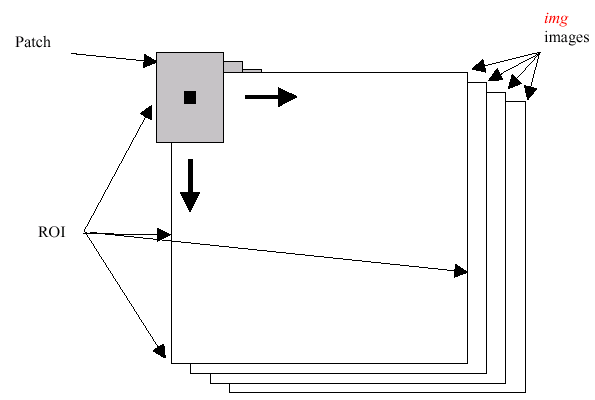
\includegraphics[width=0.5\textwidth]{pics/backprojectpatch.png}

\cvfunc{CalcProbDensity}\label{CalcProbDensity}

Divides one histogram by another

\cvexp{
void  cvCalcProbDensity( \par const CvHistogram* hist1,\par const CvHistogram* hist2,\par CvHistogram* dst\_hist,\par double scale=255 );
}{CPP}{CalcProbDensity(hist1,hist2,dst\_hst,scale=255)-> None}

\begin{description}
\cvarg{hist1}{first histogram (the divisor)}
\cvarg{hist2}{second histogram}
\cvarg{dst\_hist}{destination histogram}
\cvarg{scale}{scale factor for the destination histogram}
\end{description}

The function \texttt{CalcProbDensity} calculates the object probability density from the two histograms as:

\[
\texttt{dist\_hist}(I)=
\forkthree
{0}{if $\texttt{hist1}(I)=0$}
{\texttt{scale}}{if $\texttt{hist1}(I) \ne 0$ and $\texttt{hist2}(I) > \texttt{hist1}(I)$}
{\frac{\texttt{hist2}(I) \cdot \texttt{scale}}{\texttt{hist1}(I)}}{if $\texttt{hist1}(I) \ne 0$ and $\texttt{hist2}(I) \le \texttt{hist1}(I)$}
\]

So the destination histogram bins are within less than scale.

\cvfunc{EqualizeHist}\label{EqualizeHist}

Equalizes histogram of grayscale image

\cvexp{
void  cvEqualizeHist( const CvArr* src, CvArr* dst );
}{CPP}{EqualizeHist(src,dst)-> None}

\begin{description}
\cvarg{src}{The input 8-bit single-channel image}
\cvarg{dst}{The output image of the same size and the same data type as \texttt{src}}
\end{description}

The function \texttt{cvEqualizeHist} equalizes histogram of the input image using the following algorithm:

\begin{enumerate}
\item calculate histogram $H$ for src.
\item normalize histogram, so that the sum of histogram bins is 255.
\item compute integral of the histogram:
\[
H'_i = \sum_{0 \le j \le i} H(j)
\]
\item transform the image using $H'$ as a look-up table: $\texttt{dst}(x,y) = H'(\texttt{src}(x,y))$
\end{enumerate}

The algorithm normalizes brightness and increases contrast of the image.

\subsection{Matching}

\cvfunc{MatchTemplate}\label{MatchTemplate}

Compares template against overlapped image regions

\cvexp{
void cvMatchTemplate( \par const CvArr* image,\par const CvArr* templ,\par CvArr* result,\par int method );
}{CPP}{MatchTemplate(image,templ,result,method)-> None}

\begin{description}
\cvarg{image}{Image where the search is running. It should be 8-bit or 32-bit floating-point}
\cvarg{templ}{Searched template; must be not greater than the source image and the same data type as the image}
\cvarg{result}{A map of comparison results; single-channel 32-bit floating-point.
If \texttt{image} is $W \times H$ and
\texttt{templ} is $w \times h$ then \texttt{result} must be $(W-w+1) \times (H-h+1)$}
\cvarg{method}{Specifies the way the template must be compared with image regions (see below)}
\end{description}

The function \texttt{cvMatchTemplate} is similiar to
\cross{CalcBackProjectPatch}. It slids through \texttt{image}, compares
overlapped patches of size $w \times h$ against \texttt{templ}
using the specified method and stores the comparison results to
\texttt{result}. Here are the formulae for the different comparison
methods one may use ($I$ denotes \texttt{image}, $T$ \texttt{template},
$R$ \texttt{result}. The summation is done over template and/or the
image patch: $x' = 0...w-1, y' = 0...h-1$

% \texttt{x'=0..w-1, y'=0..h-1}):

\begin{description}
\item[method=CV\_TM\_SQDIFF]
\[ R(x,y)=\sum_{x',y'} (T(x',y')-I(x+x',y+y'))^2 \]

\item[method=CV\_TM\_SQDIFF\_NORMED]
\[ R(x,y)=\frac
{\sum_{x',y'} (T(x',y')-I(x+x',y+y'))^2}
{\sqrt{\sum_{x',y'}T(x',y')^2 \cdot \sum_{x',y'} I(x+x',y+y')^2}}
\]

\item[method=CV\_TM\_CCORR]
\[ R(x,y)=\sum_{x',y'} (T(x',y') \cdot I(x+x',y+y')) \]

\item[method=CV\_TM\_CCORR\_NORMED]
\[ R(x,y)=\frac
{\sum_{x',y'} (T(x',y') \cdot I'(x+x',y+y'))}
{\sqrt{\sum_{x',y'}T(x',y') \cdot \sum_{x',y'} I(x+x',y+y')}}
\]

\item[method=CV\_TM\_CCOEFF]
\[ R(x,y)=\sum_{x',y'} (T'(x',y') \cdot I(x+x',y+y')) \]

where
\[ 
\begin{array}{l}
T'(x',y')=T(x',y') - 1/(w \cdot h) \cdot \sum_{x'',y''} T(x'',y'')\\
I'(x+x',y+y')=I(x+x',y+y') - \frac{1}{(w \cdot h) \cdot \sum_{x'',y''} I(x+x'',y+y'')}
\end{array}
\]

\item[method=CV\_TM\_CCOEFF\_NORMED]
\[ R(x,y)=\frac
{ \sum_{x',y'} (T'(x',y') \cdot I'(x+x',y+y')) }
{ \sqrt{\sum_{x',y'}T'(x',y')^2 \cdot \sum_{x',y'} I'(x+x',y+y')^2} }
\]
\end{description}

After the function finishes comparison, the best matches can be found as global minimums (CV\_TM\_SQDIFF) or maximums (CV\_TM\_CCORR and CV\_TM\_CCOEFF) using \cross{MinMaxLoc} function. In case of color image and template summation in both numerator and each sum in denominator is done over all the channels (and separate mean values are used for each channel).

\cvfunc{MatchShapes}\label{MatchShapes}

Compares two shapes

\cvexp{
double cvMatchShapes( \par const void* object1,\par const void* object2,\par int method,\par double parameter=0 );
}{CPP}{MatchShapes(object1,object2,method,parameter=0)-> None}

\begin{description}
\cvarg{object1}{First contour or grayscale image}
\cvarg{object2}{Second contour or grayscale image}
\cvarg{method}{Comparison method, one of
 \texttt{CV\_CONTOUR\_MATCH\_I1}, 
 \texttt{CV\_CONTOURS\_MATCH\_I2} 
or 
 \texttt{CV\_CONTOURS\_MATCH\_I3}}
\cvarg{parameter}{Method-specific parameter (is not used now)}
\end{description}

The function \texttt{cvMatchShapes} compares two shapes. The 3 implemented methods all use Hu moments (see \cross{GetHuMoments}) ($A$ is \texttt{object1}, $B$ is \texttt{object2}):

\begin{description}
\item[method=CV\_CONTOUR\_MATCH\_I1]
\[ I_1(A,B) = \sum_{i=1...7} \left| \frac{1}{m^A_i} - \frac{1}{m^B_i} \right| \]

\item[method=CV\_CONTOUR\_MATCH\_I2]
\[ I_2(A,B) = \sum_{i=1...7} \left| m^A_i - m^B_i \right| \]

\item[method=CV\_CONTOUR\_MATCH\_I3]
\[ I_3(A,B) = \sum_{i=1...7} \frac{ \left| m^A_i - m^B_i \right| }{ \left| m^A_i \right| } \]
\end{description}

where

\[
\begin{array}{l}
m^A_i = sign(h^A_i) \cdot \log{h^A_i}
m^B_i = sign(h^B_i) \cdot \log{h^B_i}
\end{array}
\]

and $h^A_i, h^B_i$ are Hu moments of $A$ and $B$ respectively.

\cvfunc{CalcEMD2}\label{CalcEMD2}

Computes "minimal work" distance between two weighted point configurations

\cvexp{
float cvCalcEMD2( \par const CvArr* signature1,\par const CvArr* signature2,\par int distance\_type,\par CvDistanceFunction distance\_func=NULL,\par const CvArr* cost\_matrix=NULL,\par CvArr* flow=NULL,\par float* lower\_bound=NULL,\par void* userdata=NULL );
}{CPP}{PYTHON}

\begin{lstlisting}
typedef float (*CvDistanceFunction)(const float* f1, const float* f2, void* userdata);
\end{lstlisting}

\begin{description}
\cvarg{signature1}{First signature, $\texttt{size1}\times \texttt{dims}+1$ floating-point matrix. Each row stores the point weight followed by the point coordinates. The matrix is allowed to have a single column (weights only) if the user-defined cost matrix is used}
\cvarg{signature2}{Second signature of the same format as \texttt{signature1}, though the number of rows may be different. The total weights may be different, in this case an extra "dummy" point is added to either \texttt{signature1} or \texttt{signature2}}
\cvarg{distance\_type}{Metrics used; \texttt{CV\_DIST\_L1, CV\_DIST\_L2}, and \texttt{CV\_DIST\_C} stand for one of the standard metrics; \texttt{CV\_DIST\_USER} means that a user-defined function \texttt{distance\_func} or pre-calculated \texttt{cost\_matrix} is used}
\cvarg{distance\_func}{The user-defined distance function. It takes coordinates of two points and returns the distance between the points}
\cvarg{cost\_matrix}{The user-defined $\texttt{size1}\times \texttt{size2}$ cost matrix. At least one of \texttt{cost\_matrix} and \texttt{distance\_func} must be NULL. Also, if a cost matrix is used, lower boundary (see below) can not be calculated, because it needs a metric function}
\cvarg{flow}{The resultant $\texttt{size1} \times \texttt{size2}$ flow matrix: $\texttt{flow}_{i,j}$ is a flow from $i$ th point of \texttt{signature1} to $j$ th point of \texttt{signature2}}
\cvarg{lower\_bound}{Optional input/output parameter: lower boundary of distance between the two signatures that is a distance between mass centers. The lower boundary may not be calculated if the user-defined cost matrix is used, the total weights of point configurations are not equal, or there is the signatures consist of weights only (i.e. the signature matrices have a single column). User ''must'' initialize \texttt{*lower\_bound}. If the calculated distance between mass centers is greater or equal to \texttt{*lower\_bound} (it means that the signatures are far enough) the function does not calculate EMD. In any case \texttt{*lower\_bound} is set to the calculated distance between mass centers on return. Thus, if user wants to calculate both distance between mass centers and EMD, \texttt{*lower\_bound} should be set to 0}
\cvarg{userdata}{Pointer to optional data that is passed into the user-defined distance function}
\end{description}

The function \texttt{cvCalcEMD2} computes earth mover distance and/or
a lower boundary of the distance between the two weighted point
configurations. One of the application desctibed in \cite{RubnerSept98} is
multi-dimensional histogram comparison for image retrieval. EMD is a
transportation problem that is solved using some modification of simplex
algorithm, thus the complexity is exponential in the worst case, though,
it is much faster in average. In case of a real metric the lower boundary
can be calculated even faster (using linear-time algorithm) and it can
be used to determine roughly whether the two signatures are far enough
so that they cannot relate to the same object.

\section{Structural Analysis}

\subsection{Contour Processing Functions}

\cvfunc{ApproxChains}\label{ApproxChains}

Approximates Freeman chain(s) with polygonal curve

\cvexp{
CvSeq* cvApproxChains( \par CvSeq* src\_seq,\par CvMemStorage* storage,\par int method=CV\_CHAIN\_APPROX\_SIMPLE,\par double parameter=0,\par int minimal\_perimeter=0,\par int recursive=0 );
}{CPP}{ApproxChains(src\_seq,storage,method=CV\_CHAIN\_APPROX\_SIMPLE,parameter=0,minimal\_perimiter=0,recursive=0)-> chains}

\begin{description}
\cvarg{src\_seq}{Pointer to the chain that can refer to other chains}
\cvarg{storage}{Storage location for the resulting polylines}
\cvarg{method}{Approximation method (see the description of the function \cross{FindContours})}
\cvarg{parameter}{Method parameter (not used now)}
\cvarg{minimal\_perimeter}{Approximates only those contours whose perimeters are not less than \texttt{minimal\_perimeter}. Other chains are removed from the resulting structure}
\cvarg{recursive}{If not 0, the function approximates all chains that access can be obtained to from \texttt{src\_seq} by \texttt{h\_next} or \texttt{v\_next links}. If 0, the single chain is approximated}
\end{description}

This is a stand-alone approximation routine. The function \texttt{cvApproxChains} works exactly in the same way as \cross{FindContours} with the corresponding approximation flag. The function returns pointer to the first resultant contour. Other approximated contours, if any, can be accessed via \texttt{v\_next} or \texttt{h\_next} fields of the returned structure.

\cvfunc{StartReadChainPoints}\label{StartReadChainPoints}

Initializes chain reader

\cvexp{
void cvStartReadChainPoints( CvChain* chain, CvChainPtReader* reader );
}{CPP}{PYTHON}

The function \texttt{cvStartReadChainPoints} initializes a special reader

\cvfunc{ReadChainPoint}\label{ReadChainPoint}

Gets next chain point

\cvexp{
CvPoint cvReadChainPoint( CvChainPtReader* reader );
}{CPP}{PYTHON}

\begin{description}
\cvarg{reader}{Chain reader state}
\end{description}

The function \texttt{cvReadChainPoint} returns the current chain point and updates the reader position.

\cvfunc{ApproxPoly}\label{ApproxPoly}

Approximates polygonal curve(s) with desired precision

\cvexp{
CvSeq* cvApproxPoly( \par const void* src\_seq,\par int header\_size,\par CvMemStorage* storage,\par int method,\par double parameter,\par int parameter2=0 );
}{CPP}{PYTHON}

\begin{description}
\cvarg{src\_seq}{Sequence of array of points}
\cvarg{header\_size}{Header size of approximated curve[s]}
\cvarg{storage}{Container for approximated contours. If it is NULL, the input sequences' storage is used}
\cvarg{method}{Approximation method; only \texttt{CV\_POLY\_APPROX\_DP} is supported, that corresponds to Douglas-Peucker algorithm}
\cvarg{parameter}{Method-specific parameter; in case of \texttt{CV\_POLY\_APPROX\_DP} it is a desired approximation accuracy}
\cvarg{parameter2}{If case if \texttt{src\_seq} is sequence it means whether the single sequence should be approximated or all sequences on the same level or below \texttt{src\_seq} (see \cross{FindContours} for description of hierarchical contour structures). And if \texttt{src\_seq} is array CvMat* of points, the parameter specifies whether the curve is closed (\texttt{parameter2}!=0) or not (\texttt{parameter2} =0)}
\end{description}

The function \texttt{cvApproxPoly} approximates one or more curves and returns the approximation result[s]. In case of multiple curves approximation the resultant tree will have the same structure as the input one (1:1 correspondence).

\cvfunc{BoundingRect}\label{BoundingRect}

Calculates up-right bounding rectangle of point set

\cvexp{
CvRect cvBoundingRect( CvArr* points, int update=0 );
}{CPP}{BoundingRect(points,update=0)-> CvRect}

\begin{description}
\cvarg{points}{2D point set, either a sequence or vector (\texttt{CvMat}) of points}
\cvarg{update}{The update flag. See below.}
\end{description}

The function \texttt{cvBoundingRect} returns the up-right bounding rectangle for 2d point set.
Here is list of possible combination of the flag values and type of \texttt{points}:

\begin{tabular}{|c|c|p{3in}|}
\hline
update & points & action \\ \hline
0 & \texttt{CvContour\*} & the bounding rectangle is not calculated, but it is taken from \texttt{rect} field of the contour header.\\ \hline
1 & \texttt{CvContour\*} & the bounding rectangle is calculated and written to \texttt{rect} field of the contour header.\\ \hline
0 & \texttt{CvSeq\*} or \texttt{CvMat\*} & the bounding rectangle is calculated and returned.\\ \hline
1 & \texttt{CvSeq\*} or \texttt{CvMat\*} & runtime error is raised.\\ \hline
\end{tabular}

\cvfunc{ContourArea}\label{ContourArea}

Calculates area of the whole contour or contour section

\cvexp{
double cvContourArea( \par const CvArr* contour, \par CvSlice slice=CV\_WHOLE\_SEQ );
}{CPP}{ContourAres(contour,slice=CV\_WHOLE\_SEQ)-> double}

\begin{description}
\cvarg{contour}{Contour (sequence or array of vertices)}
\cvarg{slice}{Starting and ending points of the contour section of interest, by default area of the whole contour is calculated}
\end{description}

The function \texttt{cvContourArea} calculates area of the whole contour
or contour section. In the latter case the total area bounded by the
contour arc and the chord connecting the 2 selected points is calculated
as shown on the picture below:

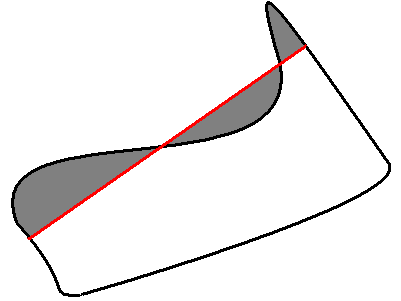
\includegraphics[width=0.5\textwidth]{pics/contoursecarea.png}

Orientation of the contour affects the area sign, thus the function may return \emph{negative} result. Use \texttt{fabs()} function from C runtime to get the absolute value of area.

\cvfunc{ArcLength}\label{ArcLength}

Calculates contour perimeter or curve length

\cvexp{
double cvArcLength( \par const void* curve,\par CvSlice slice=CV\_WHOLE\_SEQ,\par int is\_closed=-1 );
}{CPP}{ArcLength(curve,slice=CV\_WHOLE\_SEQ,is\_closed=-1)-> double}

\begin{description}
\cvarg{curve}{Sequence or array of the curve points}
\cvarg{slice}{Starting and ending points of the curve, by default the whole curve length is calculated}
\cvarg{is\_closed}{Indicates whether the curve is closed or not. There are 3 cases:
\begin{itemize}
  \item $\texttt{is\_closed} =0$ the curve is assumed to be unclosed.
  \item $\texttt{is\_closed}>0$ the curve is assumed to be closed.
  \item $\texttt{is\_closed}<0$ if curve is sequence, the flag \texttt{CV\_SEQ\_FLAG\_CLOSED} of \texttt{((CvSeq*)curve)->flags} is checked to determine if the curve is closed or not, otherwise (curve is represented by array (CvMat*) of points) it is assumed to be unclosed.
\end{itemize}}
\end{description}

The function \texttt{cvArcLength} calculates length or curve as sum of lengths of segments between subsequent points

\cvfunc{CreateContourTree}\label{CreateContourTree}

Creates hierarchical representation of contour

\cvexp{
CvContourTree* cvCreateContourTree( /par const CvSeq* contour,\par CvMemStorage* storage,\par double threshold );
}{CPP}{CreateCountourTree(contour,storage,threshold)-> contour\_tree}

\begin{description}
\cvarg{contour}{Input contour}
\cvarg{storage}{Container for output tree}
\cvarg{threshold}{Approximation accuracy}
\end{description}

The function \texttt{cvCreateContourTree} creates binary tree representation for the input \texttt{contour} and returns the pointer to its root. If the parameter \texttt{threshold} is less than or equal to 0, the function creates full binary tree representation. If the threshold is greater than 0, the function creates representation with the precision \texttt{threshold}: if the vertices with the interceptive area of its base line are less than \texttt{threshold}, the tree should not be built any further. The function returns the created tree.

\cvfunc{ContourFromContourTree}\label{ContourFromContourTree}

Restores contour from tree

\cvexp{
CvSeq* cvContourFromContourTree( \par const CvContourTree* tree,\par CvMemStorage* storage,\par CvTermCriteria criteria );
}{CPP}{ContourFromContourTree(tree,storage,criteria)-> contour}

\begin{description}
\cvarg{tree}{Contour tree}
\cvarg{storage}{Container for the reconstructed contour}
\cvarg{criteria}{Criteria, where to stop reconstruction}
\end{description}

The function \texttt{cvContourFromContourTree} restores the contour from its binary tree representation. The parameter \texttt{criteria} determines the accuracy and/or the number of tree levels used for reconstruction, so it is possible to build approximated contour. The function returns reconstructed contour.

\cvfunc{MatchContourTrees}\label{MatchContourTrees}

Compares two contours using their tree representations

\cvexp{
double cvMatchContourTrees( \par const CvContourTree* tree1,\par const CvContourTree* tree2,\par int method,\par double threshold );
}{CPP}{MatchContourTrees(tree1,tree2,method,threshold)-> double}

\begin{description}
\cvarg{tree1}{First contour tree}
\cvarg{tree2}{Second contour tree}
\cvarg{method}{Similarity measure, only \texttt{CV\_CONTOUR\_TREES\_MATCH\_I1} is supported}
\cvarg{threshold}{Similarity threshold}
\end{description}

The function \texttt{cvMatchContourTrees} calculates the value of the matching measure for two contour trees. The similarity measure is calculated level by level from the binary tree roots. If at the certain level difference between contours becomes less than \texttt{threshold}, the reconstruction process is interrupted and the current difference is returned.

\subsection{Computational Geometry}

\cvfunc{MaxRect}\label{MaxRect}

Finds bounding rectangle for two given rectangles

\cvexp{
CvRect cvMaxRect( \par const CvRect* rect1,\par const CvRect* rect2 );
}{CPP}{MaxRect(rect1,rect2)-> CvRect}

\begin{description}
\cvarg{rect1}{First rectangle}
\cvarg{rect2}{Second rectangle}
\end{description}

The function \texttt{cvMaxRect} finds minimum area rectangle that contains both input rectangles inside:

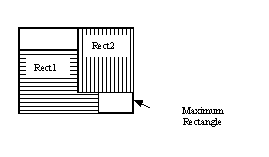
\includegraphics[width=0.5\textwidth]{pics/maxrect.png}

\cvfunc{CvBox2D}\label{CvBox2D}

Rotated 2D box

\begin{lstlisting}
typedef struct CvBox2D
{
    CvPoint2D32f center;  /* center of the box */
    CvSize2D32f  size;    /* box width and length */
    float angle;          /* angle between the horizontal axis
                             and the first side (i.e. length) in radians */
}
CvBox2D;
\end{lstlisting}

\cvfunc{PointSeqFromMat}\label{PointSeqFromMat}

Initializes point sequence header from a point vector

\cvexp{
CvSeq* cvPointSeqFromMat( \par int seq\_kind,\par const CvArr* mat,\par CvContour* contour\_header,\par CvSeqBlock* block );
}{CPP}{PYTHON}

\begin{description}
\cvarg{seq\_kind}{Type of the point sequence: point set (0), a curve (\texttt{CV\_SEQ\_KIND\_CURVE}), closed curve (\texttt{CV\_SEQ\_KIND\_CURVE+CV\_SEQ\_FLAG\_CLOSED}) etc.}
\cvarg{mat}{Input matrix. It should be continuous 1-dimensional vector of points, that is, it should have type \texttt{CV\_32SC2} or \texttt{CV\_32FC2}}
\cvarg{contour\_header}{Contour header, initialized by the function}
\cvarg{block}{Sequence block header, initialized by the function}
\end{description}

The function \texttt{cvPointSeqFromMat} initializes sequence
header to create a "virtual" sequence which elements reside in
the specified matrix. No data is copied. The initialized sequence
header may be passed to any function that takes a point sequence
on input. No extra elements could be added to the sequence,
but some may be removed. The function is a specialized variant of
\cross{MakeSeqHeaderForArray} and uses
the latter internally. It returns pointer to the initialized contour
header. Note that the bounding rectangle (field \texttt{rect} of
\texttt{CvContour} strucuture is not initialized by the function. If
you need one, use \cross{BoundingRect}.

Here is the simple usage example.

\begin{lstlisting}
CvContour header;
CvSeqBlock block;
CvMat* vector = cvCreateMat( 1, 3, CV_32SC2 );

CV_MAT_ELEM( *vector, CvPoint, 0, 0 ) = cvPoint(100,100);
CV_MAT_ELEM( *vector, CvPoint, 0, 1 ) = cvPoint(100,200);
CV_MAT_ELEM( *vector, CvPoint, 0, 2 ) = cvPoint(200,100);

IplImage* img = cvCreateImage( cvSize(300,300), 8, 3 );
cvZero(img);

cvDrawContours( img,
    cvPointSeqFromMat(CV_SEQ_KIND_CURVE+CV_SEQ_FLAG_CLOSED,
                      vector,
                      &header,
                      &block),
                CV_RGB(255,0,0),
                CV_RGB(255,0,0),
                0, 3, 8, cvPoint(0,0));
\end{lstlisting}

\cvfunc{CvBox2D}\label{CvBox2D}

Rotated 2D box

\begin{lstlisting}
typedef struct CvBox2D
{
    CvPoint2D32f center;  /* center of the box */
    CvSize2D32f  size;    /* box width and length */
    float angle;          /* angle between the horizontal axis
                             and the first side (i.e. length) in radians */
}
CvBox2D;
\end{lstlisting}

\cvfunc{BoxPoints}\label{BoxPoints}

Finds box vertices

\cvexp{
void cvBoxPoints( \par CvBox2D box,\par CvPoint2D32f pt[4] );
}{CPP}{BoxPoints(box)-> pt}

\begin{description}
\cvarg{box}{Box}
\cvarg{pt}{Array of vertices}
\end{description}

The function \texttt{cvBoxPoints} calculates vertices of the input 2d box. Here is the function code:

\begin{lstlisting}
void cvBoxPoints( CvBox2D box, CvPoint2D32f pt[4] )
{
    float a = (float)cos(box.angle)*0.5f;
    float b = (float)sin(box.angle)*0.5f;

    pt[0].x = box.center.x - a*box.size.height - b*box.size.width;
    pt[0].y = box.center.y + b*box.size.height - a*box.size.width;
    pt[1].x = box.center.x + a*box.size.height - b*box.size.width;
    pt[1].y = box.center.y - b*box.size.height - a*box.size.width;
    pt[2].x = 2*box.center.x - pt[0].x;
    pt[2].y = 2*box.center.y - pt[0].y;
    pt[3].x = 2*box.center.x - pt[1].x;
    pt[3].y = 2*box.center.y - pt[1].y;
}
\end{lstlisting}

\cvfunc{FitEllipse}\label{FitEllipse}

Fits ellipse to set of 2D points

\cvexp{
CvBox2D cvFitEllipse2( \par const CvArr* points );
}{CPP}{FitEllipse2(points)-> Box2D}

\begin{description}
\cvarg{points}{Sequence or array of points}
\end{description}

The function \texttt{cvFitEllipse} calculates ellipse that fits best
(in least-squares sense) to a set of 2D points. The meaning of the
returned structure fields is similar to those in \cross{Ellipse} except
that \texttt{size} stores the full lengths of the ellipse axises,
not half-lengths

\cvfunc{FitLine}\label{FitLine}

Fits line to 2D or 3D point set

\cvexp{
void  cvFitLine( \par const CvArr* points,\par int dist\_type,\par double param,\par double reps,\par double aeps,\par float* line );
}{CPP}{PYTHON}

\begin{description}
\cvarg{points}{Sequence or array of 2D or 3D points with 32-bit integer or floating-point coordinates}
\cvarg{dist\_type}{The distance used for fitting (see the discussion)}
\cvarg{param}{Numerical parameter (\texttt{C}) for some types of distances, if 0 then some optimal value is chosen}
\cvarg{reps, aeps}{Sufficient accuracy for radius (distance between the coordinate origin and the line) and angle, respectively, 0.01 would be a good defaults for both. is used}
\cvarg{line}{The output line parameters. In case of 2d fitting it is array of 4 floats \texttt{(vx, vy, x0, y0)} where \texttt{(vx, vy)} is a normalized vector collinear to the line and \texttt{(x0, y0)} is some point on the line. In case of 3D fitting it is array of 6 floats \texttt{(vx, vy, vz, x0, y0, z0)} where \texttt{(vx, vy, vz)} is a normalized vector collinear to the line and \texttt{(x0, y0, z0)} is some point on the line}
\end{description}

The function \texttt{cvFitLine} fits line to 2D or 3D point set by minimizing $\sum_i \rho(r_i)$ where $r_i$ is distance between $i$ th point and the line and $\rho(r)$ is a distance function, one of:

\begin{description}

\item[dist\_type=CV\_DIST\_L2]
\[ \rho(r) = r^2/2 \quad \text{(the simplest and the fastest least-squares method)} \]

\item[dist\_type=CV\_DIST\_L1]
\[ \rho(r) = r \]

\item[dist\_type=CV\_DIST\_L12]
\[ \rho(r) = 2 \cdot (\sqrt{1 + \frac{r^2}{2}} - 1) \]

\item[dist\_type=CV\_DIST\_FAIR]
\[ \rho\left(r\right) = C^2 \cdot \left( \frac{r}{C} - \log{\left(1 + \frac{r}{C}\right)}\right) \quad \text{where} \quad C=1.3998 \]

\item[dist\_type=CV\_DIST\_WELSCH]
\[ \rho\left(r\right) = \frac{C^2}{2} \cdot \left( 1 - \exp{\left(-\left(\frac{r}{C}\right)^2\right)}\right) \quad \text{where} \quad C=2.9846 \]

\item[dist\_type=CV\_DIST\_HUBER]
\[ \rho(r) = \fork
{r^2/2}{if $r < C$}
{C \cdot (r-C/2)}{otherwise}  \quad \text{where} \quad C=1.345
\]
\end{description}

\cvfunc{ConvexHull2}\label{ConvexHull2}

Finds convex hull of point set

\cvexp{
CvSeq* cvConvexHull2( \par const CvArr* input,\par void* hull\_storage=NULL,\par int orientation=CV\_CLOCKWISE,\par int return\_points=0 );
}{CPP}{ConvexHull2(points,storage,orientaton=CV\_CLOCKWISE,return\_points=0)-> convex\_hull}

\begin{description}
\cvarg{points}{Sequence or array of 2D points with 32-bit integer or floating-point coordinates}
\cvarg{hull\_storage}{The destination array (CvMat*) or memory storage (CvMemStorage*) that will store the convex hull. If it is array, it should be 1d and have the same number of elements as the input array/sequence. On output the header is modified so to truncate the array downto the hull size.  If hull\_storage is NULL then the convex hull will be stored in the same storage as the input sequence}
\cvarg{orientation}{Desired orientation of convex hull: \texttt{CV\_CLOCKWISE} or \texttt{CV\_COUNTER\_CLOCKWISE}}
\cvarg{return\_points}{If non-zero, the points themselves will be stored in the hull instead of indices if \texttt{hull\_storage} is array, or pointers if \texttt{hull\_storage} is memory storage}
\end{description}

The function \texttt{cvConvexHull2} finds convex hull of 2D point set using Sklansky?s algorithm. If \texttt{hull\_storage} is memory storage, the function creates a sequence containing the hull points or pointers to them, depending on \texttt{return\_points} value and returns the sequence on output.  If \texttt{hull\_storage} is a CvMat, the function returns NULL.

% ===== Example. Building convex hull for a sequence or array of points =====
\begin{lstlisting}
#include "cv.h"
#include "highgui.h"
#include <stdlib.h>

#define ARRAY  0 /* switch between array/sequence method by replacing 0<=>1 */

void main( int argc, char** argv )
{
    IplImage* img = cvCreateImage( cvSize( 500, 500 ), 8, 3 );
    cvNamedWindow( "hull", 1 );

#if !ARRAY
        CvMemStorage* storage = cvCreateMemStorage();
#endif

    for(;;)
    {
        int i, count = rand()%100 + 1, hullcount;
        CvPoint pt0;
#if !ARRAY
        CvSeq* ptseq = cvCreateSeq( CV_SEQ_KIND_GENERIC|CV_32SC2,
                                    sizeof(CvContour),
                                    sizeof(CvPoint),
                                    storage );
        CvSeq* hull;

        for( i = 0; i < count; i++ )
        {
            pt0.x = rand() % (img->width/2) + img->width/4;
            pt0.y = rand() % (img->height/2) + img->height/4;
            cvSeqPush( ptseq, &pt0 );
        }
        hull = cvConvexHull2( ptseq, 0, CV_CLOCKWISE, 0 );
        hullcount = hull->total;
#else
        CvPoint* points = (CvPoint*)malloc( count * sizeof(points[0]));
        int* hull = (int*)malloc( count * sizeof(hull[0]));
        CvMat point_mat = cvMat( 1, count, CV_32SC2, points );
        CvMat hull_mat = cvMat( 1, count, CV_32SC1, hull );

        for( i = 0; i < count; i++ )
        {
            pt0.x = rand() % (img->width/2) + img->width/4;
            pt0.y = rand() % (img->height/2) + img->height/4;
            points[i] = pt0;
        }
        cvConvexHull2( &point_mat, &hull_mat, CV_CLOCKWISE, 0 );
        hullcount = hull_mat.cols;
#endif
        cvZero( img );
        for( i = 0; i < count; i++ )
        {
#if !ARRAY
            pt0 = *CV_GET_SEQ_ELEM( CvPoint, ptseq, i );
#else
            pt0 = points[i];
#endif
            cvCircle( img, pt0, 2, CV_RGB( 255, 0, 0 ), CV_FILLED );
        }

#if !ARRAY
        pt0 = **CV_GET_SEQ_ELEM( CvPoint*, hull, hullcount - 1 );
#else
        pt0 = points[hull[hullcount-1]];
#endif

        for( i = 0; i < hullcount; i++ )
        {
#if !ARRAY
            CvPoint pt = **CV_GET_SEQ_ELEM( CvPoint*, hull, i );
#else
            CvPoint pt = points[hull[i]];
#endif
            cvLine( img, pt0, pt, CV_RGB( 0, 255, 0 ));
            pt0 = pt;
        }

        cvShowImage( "hull", img );

        int key = cvWaitKey(0);
        if( key == 27 ) // 'ESC'
            break;

#if !ARRAY
        cvClearMemStorage( storage );
#else
        free( points );
        free( hull );
#endif
    }
}
\end{lstlisting}

\cvfunc{CheckContourConvexity}\label{CheckContourConvexity}

Tests contour convex

\cvexp{
int cvCheckContourConvexity( const CvArr* contour );
}{CPP}{CheckContourConvexity(contour)-> int}

\begin{description}
\cvarg{contour}{Tested contour (sequence or array of points)}
\end{description}

The function \texttt{cvCheckContourConvexity} tests whether the input contour is convex or not. The contour must be simple, i.e. without self-intersections.

\cvstruct{CvConvexityDefect}\label{CvConvexityDefect}

Structure describing a single contour convexity detect

\begin{lstlisting}
typedef struct CvConvexityDefect
{
    CvPoint* start; /* point of the contour where the defect begins */
    CvPoint* end; /* point of the contour where the defect ends */
    CvPoint* depth_point; /* the farthest from the convex hull point within the defect */
    float depth; /* distance between the farthest point and the convex hull */
} CvConvexityDefect;
\end{lstlisting}

% ===== Picture. Convexity defects of hand contour. =====
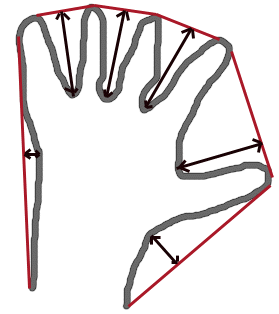
\includegraphics[width=0.5\textwidth]{pics/defects.png}

\cvfunc{ConvexityDefects}\label{ConvexityDefects}

Finds convexity defects of contour

\cvexp{
CvSeq* cvConvexityDefects( \par const CvArr* contour,\par const CvArr* convexhull,\par CvMemStorage* storage=NULL );
}{CPP}{ConvexityDefects(contour,convexhull,storage)-> convexity\_defects}

\begin{description}
\cvarg{contour}{Input contour}
\cvarg{convexhull}{Convex hull obtained using \cross{ConvexHull2} that should contain pointers or indices to the contour points, not the hull points themselves, i.e. \texttt{return\_points} parameter in \cross{ConvexHull2} should be 0}
\cvarg{storage}{Container for output sequence of convexity defects. If it is NULL, contour or hull (in that order) storage is used}
\end{description}

The function \texttt{ConvexityDefects} finds all convexity defects of the input contour and returns a sequence of the CvConvexityDefect structures.

\cvfunc{PointPolygonTest}\label{PointPolygonTest}

Point in contour test

\cvexp{
double cvPointPolygonTest( \par const CvArr* contour,\par CvPoint2D32f pt,\par int measure\_dist );
}{CPP}{PointPolygonTest(contour,pt,measure\_dist)-> double}

\begin{description}
\cvarg{contour}{Input contour}
\cvarg{pt}{The point tested against the contour}
\cvarg{measure\_dist}{If it is non-zero, the function estimates distance from the point to the nearest contour edge}
\end{description}

The function \texttt{cvPointPolygonTest} determines whether the
point is inside contour, outside, or lies on an edge (or coinsides
with a vertex). It returns positive, negative or zero value,
correspondingly. When $\texttt{measure\_dist} =0$, the return value
is +1, -1 and 0, respectively. When $\texttt{measure\_dist} \ne 0$,
it is a signed distance between the point and the nearest contour
edge.

Here is the sample output of the function, where each image pixel is tested against the contour.

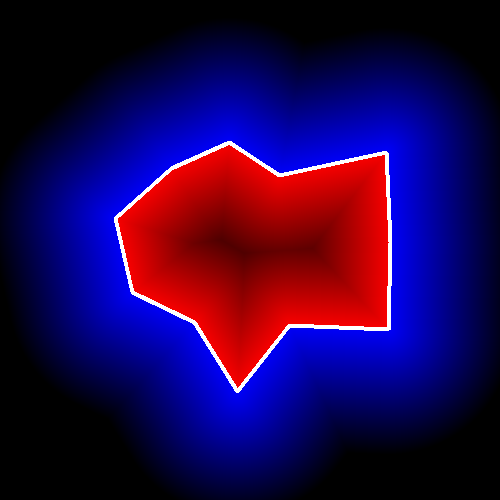
\includegraphics[width=0.5\textwidth]{pics/pointpolygon.png}

\cvfunc{MinAreaRect2}\label{MinAreaRect2}

Finds circumscribed rectangle of minimal area for given 2D point set

\cvexp{
CvBox2D  cvMinAreaRect2( \par const CvArr* points,\par CvMemStorage* storage=NULL );
}{CPP}{MinAreaRect2(points,storage)-> CvBox2D}

\begin{description}
\cvarg{points}{Sequence or array of points}
\cvarg{storage}{Optional temporary memory storage}
\end{description}

The function \texttt{cvMinAreaRect2} finds a circumscribed rectangle of the minimal area for 2D point set by building convex hull for the set and applying rotating calipers technique to the hull.

% ===== Picture. Minimal-area bounding rectangle for contour =====
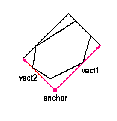
\includegraphics[width=0.5\textwidth]{pics/minareabox.png}

\cvfunc{MinEnclosingCircle}\label{MinEnclosingCircle}

Finds circumscribed circle of minimal area for given 2D point set

\cvexp{
int cvMinEnclosingCircle( \par const CvArr* points,\par CvPoint2D32f* center,\par float* radius );
}{CPP}{MinEnclosingCircle(points)-> int,center,radius}

\begin{description}
\cvarg{points}{Sequence or array of 2D points}
\cvarg{center}{Output parameter. The center of the enclosing circle}
\cvarg{radius}{Output parameter. The radius of the enclosing circle}
\end{description}

The function \texttt{cvMinEnclosingCircle} finds the minimal circumscribed
circle for 2D point set using iterative algorithm. It returns nonzero
if the resultant circle contains all the input points and zero otherwise
(i.e. algorithm failed).

\cvfunc{CalcPGH}\label{CalcPGH}

Calculates pair-wise geometrical histogram for contour

\cvexp{
void cvCalcPGH( const CvSeq* contour, CvHistogram* hist );
}{CPP}{CalcPGH(contour,hist)-> None}

\begin{description}
\cvarg{contour}{Input contour. Currently, only integer point coordinates are allowed}
\cvarg{hist}{Calculated histogram; must be two-dimensional}
\end{description}

The function \texttt{cvCalcPGH} calculates
2D pair-wise geometrical histogram (PGH), described in
Iivarinen97
for the contour. The algorithm considers every pair of the contour
edges. The angle between the edges and the minimum/maximum distances
are determined for every pair. To do this each of the edges in turn
is taken as the base, while the function loops through all the other
edges. When the base edge and any other edge are considered, the minimum
and maximum distances from the points on the non-base edge and line of
the base edge are selected. The angle between the edges defines the row
of the histogram in which all the bins that correspond to the distance
between the calculated minimum and maximum distances are incremented
(that is, the histogram is transposed relatively to [Iivarninen97]
definition). The histogram can be used for contour matching.

\subsection{Planar Subdivisions}

\cvstruct{CvSubdiv2D}\label{CvSubdiv2D}

Planar subdivision

\begin{lstlisting}
#define CV_SUBDIV2D_FIELDS()    \
    CV_GRAPH_FIELDS()           \
    int  quad_edges;            \
    int  is_geometry_valid;     \
    CvSubdiv2DEdge recent_edge; \
    CvPoint2D32f  topleft;      \
    CvPoint2D32f  bottomright;

typedef struct CvSubdiv2D
{
    CV_SUBDIV2D_FIELDS()
}
CvSubdiv2D;
\end{lstlisting}

Planar subdivision is a subdivision of a plane into a set of
non-overlapped regions (facets) that cover the whole plane. The above
structure describes a subdivision built on 2d point set, where the points
are linked together and form a planar graph, which, together with a few
edges connecting exterior subdivision points (namely, convex hull points)
with infinity, subdivides a plane into facets by its edges.

For every subdivision there exists dual subdivision there facets and
points (subdivision vertices) swap their roles, that is, a facet is
treated as a vertex (called virtual point below) of dual subdivision and
the original subdivision vertices become facets. On the picture below
original subdivision is marked with solid lines and dual subdivision
with dot lines

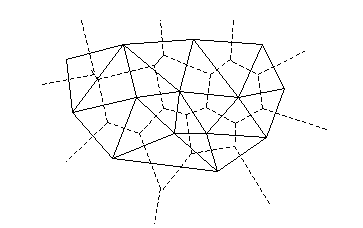
\includegraphics[width=0.5\textwidth]{pics/subdiv.png}

OpenCV subdivides plane into triangles using Delaunay's
algorithm. Subdivision is built iteratively starting from a dummy
triangle that includes all the subdivision points for sure. In this
case the dual subdivision is Voronoi diagram of input 2d point set. The
subdivisions can be used for 3d piece-wise transformation of a plane,
morphing, fast location of points on the plane, building special graphs
(such as NNG,RNG) etc.

\cvstruct{CvQuadEdge2D}\label{CvQuadEdge2D}

Quad-edge of planar subdivision

\begin{lstlisting}
/* one of edges within quad-edge, lower 2 bits is index (0..3)
   and upper bits are quad-edge pointer */
typedef long CvSubdiv2DEdge;

/* quad-edge structure fields */
#define CV_QUADEDGE2D_FIELDS()     \
    int flags;                     \
    struct CvSubdiv2DPoint* pt[4]; \
    CvSubdiv2DEdge  next[4];

typedef struct CvQuadEdge2D
{
    CV_QUADEDGE2D_FIELDS()
}
CvQuadEdge2D;

\end{lstlisting}

Quad-edge is a basic element of subdivision, it contains four edges (e, eRot, reversed e and reversed eRot):

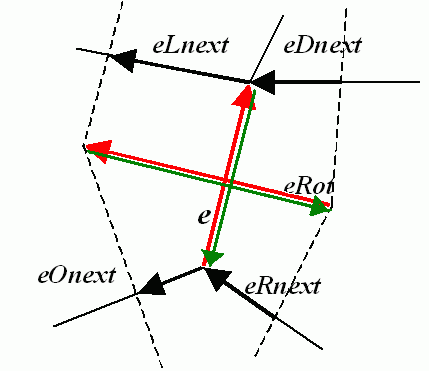
\includegraphics[width=0.5\textwidth]{pics/quadedge.png}

\cvstruct{CvSubdiv2DPoint}\label{CvSubdiv2DPoint}

Point of original or dual subdivision

\begin{lstlisting}
#define CV_SUBDIV2D_POINT_FIELDS()\
    int            flags;      \
    CvSubdiv2DEdge first;      \
    CvPoint2D32f   pt;

#define CV_SUBDIV2D_VIRTUAL_POINT_FLAG (1 << 30)

typedef struct CvSubdiv2DPoint
{
    CV_SUBDIV2D_POINT_FIELDS()
}
CvSubdiv2DPoint;
\end{lstlisting}

\cvfunc{Subdiv2DGetEdge}\label{Subdiv2DGetEdge}

Returns one of edges related to given

\cvexp{
CvSubdiv2DEdge  cvSubdiv2DGetEdge( CvSubdiv2DEdge edge, CvNextEdgeType type );


}{CPP}{Subdiv2DGetEdge(edge,type)-> CvSubdiv2DEdge}
\begin{lstlisting}
#define cvSubdiv2DNextEdge( edge ) cvSubdiv2DGetEdge( edge, CV_NEXT_AROUND_ORG )
\end{lstlisting}

\begin{description}
\cvarg{edge}{Subdivision edge (not a quad-edge)}
\cvarg{type}{Specifies, which of related edges to return, one of:}
\begin{description}
  \cvarg{CV\_NEXT\_AROUND\_ORG}{next around the edge origin (\texttt{eOnext} on the picture above if \texttt{e} is the input edge)}
  \cvarg{CV\_NEXT\_AROUND\_DST}{next around the edge vertex (\texttt{eDnext})}
  \cvarg{CV\_PREV\_AROUND\_ORG}{previous around the edge origin (reversed \texttt{eRnext})}
  \cvarg{CV\_PREV\_AROUND\_DST}{previous around the edge destination (reversed \texttt{eLnext})}
  \cvarg{CV\_NEXT\_AROUND\_LEFT}{next around the left facet (\texttt{eLnext})}
  \cvarg{CV\_NEXT\_AROUND\_RIGHT}{next around the right facet (\texttt{eRnext})}
  \cvarg{CV\_PREV\_AROUND\_LEFT}{previous around the left facet (reversed \texttt{eOnext})}
  \cvarg{CV\_PREV\_AROUND\_RIGHT}{previous around the right facet (reversed \texttt{eDnext})}
\end{description}
\end{description}

The function \texttt{cvSubdiv2DGetEdge} returns one the edges related to the input edge.

\cvfunc{Subdiv2DRotateEdge}\label{Subdiv2DRotateEdge}

Returns another edge of the same quad-edge

\cvexp{
CvSubdiv2DEdge  cvSubdiv2DRotateEdge( \par CvSubdiv2DEdge edge,\par int rotate );
}{CPP}{Subdiv2DRotateEdge(edge,rotate)-> CvSubdiv2DEdge}

\begin{description}
\cvarg{edge}{Subdivision edge (not a quad-edge)}
\cvarg{type}{Specifies, which of edges of the same quad-edge as the input one to return, one of:
\begin{description}
  \cvarg{0}{the input edge (\texttt{e} on the picture above if \texttt{e} is the input edge)}
  \cvarg{1}{the rotated edge (\texttt{eRot})}
  \cvarg{2}{the reversed edge (reversed \texttt{e} (in green))}
  \cvarg{3}{the reversed rotated edge (reversed \texttt{eRot} (in green))}
\end{description}}
\end{description}

The function \texttt{cvSubdiv2DRotateEdge} returns one the edges of the same quad-edge as the input edge.

\cvfunc{Subdiv2DEdgeOrg}\label{Subdiv2DEdgeOrg}

Returns edge origin

\cvexp{
CvSubdiv2DPoint* cvSubdiv2DEdgeOrg( \par CvSubdiv2DEdge edge );
}{CPP}{Subdiv2DEdgeOrg(edge)-> point}

\begin{description}
\cvarg{edge}{Subdivision edge (not a quad-edge)}
\end{description}

The function \texttt{cvSubdiv2DEdgeOrg} returns the edge
origin. The returned pointer may be NULL if the edge is from dual
subdivision and the virtual point coordinates are not calculated
yet. The virtual points can be calculated using function
\cross{CalcSubdivVoronoi2D}.

\cvfunc{Subdiv2DEdgeDst}\label{Subdiv2DEdgeDst}

Returns edge destination

\cvexp{
CvSubdiv2DPoint* cvSubdiv2DEdgeDst( \par CvSubdiv2DEdge edge );
}{CPP}{Subdiv2DEdgeDist(edge)-> point}

\begin{description}
\cvarg{edge}{Subdivision edge (not a quad-edge)}
\end{description}

The function \texttt{cvSubdiv2DEdgeDst} returns the edge destination. The
returned pointer may be NULL if the edge is from dual subdivision and
the virtual point coordinates are not calculated yet. The virtual points
can be calculated using function \cross{CalcSubdivVoronoi2D}.

\cvfunc{CreateSubdivDelaunay2D}\label{CreateSubdivDelaunay2D}

Creates empty Delaunay triangulation

\cvexp{
CvSubdiv2D* cvCreateSubdivDelaunay2D( \par CvRect rect,\par CvMemStorage* storage );
}{CPP}{CreateSubdivDelaunay2D(rect,storage)-> delaunay\_triangulation}

\begin{description}
\cvarg{rect}{Rectangle that includes all the 2d points that are to be added to subdivision}
\cvarg{storage}{Container for subdivision}
\end{description}

The function \texttt{CreateSubdivDelaunay2D} creates an empty Delaunay
subdivision, where 2d points can be added further using function
\cross{SubdivDelaunay2DInsert}. All the points to be added must be within
the specified rectangle, otherwise a runtime error will be raised.

\cvfunc{SubdivDelaunay2DInsert}\label{SubdivDelaunay2DInsert}

Inserts a single point to Delaunay triangulation

\cvexp{
CvSubdiv2DPoint*  cvSubdivDelaunay2DInsert( \par CvSubdiv2D* subdiv,\par CvPoint2D32f pt);
}{CPP}{SubdivDelaunay2DInsert(subdiv,pt)-> point}

\begin{description}
\cvarg{subdiv}{Delaunay subdivision created by function \cross{CreateSubdivDelaunay2D}}
\cvarg{pt}{Inserted point}
\end{description}

The function \texttt{cvSubdivDelaunay2DInsert} inserts a single point to subdivision and modifies the subdivision topology appropriately. If a points with same coordinates exists already, no new points is added. The function returns pointer to the allocated point. No virtual points coordinates is calculated at this stage.

\cvfunc{Subdiv2DLocate}\label{Subdiv2DLocate}

Inserts a single point to Delaunay triangulation

\cvexp{
CvSubdiv2DPointLocation  cvSubdiv2DLocate( \par CvSubdiv2D* subdiv,\par CvPoint2D32f pt,\par CvSubdiv2DEdge* edge,\par CvSubdiv2DPoint** vertex=NULL );
}{CPP}{PYTHON}

\begin{description}
\cvarg{subdiv}{Delaunay or another subdivision}
\cvarg{pt}{The point to locate}
\cvarg{edge}{The output edge the point falls onto or right to}
\cvarg{vertex}{Optional output vertex double pointer the input point coinsides with}
\end{description}

The function \texttt{cvSubdiv2DLocate} locates input point within subdivision. There are 5 cases:

\begin{itemize}
 \item point falls into some facet. The function returns \\texttt{CV\_PTLOC\_INSIDE} and \texttt{*edge} will contain one of edges of the facet.
 \item point falls onto the edge. The function returns \\texttt{CV\_PTLOC\_ON\_EDGE} and \texttt{*edge} will contain this edge.
 \item point coinsides with one of subdivision vertices. The function returns \\texttt{CV\_PTLOC\_VERTEX} and \texttt{*vertex} will contain pointer to the vertex.
 \item point is outside the subdivsion reference rectangle. The function returns \\texttt{CV\_PTLOC\_OUTSIDE\_RECT} and no pointers is filled.
 \item one of input arguments is invalid. Runtime error is raised or, if silent or "parent" error processing mode is selected, \\texttt{CV\_PTLOC\_ERROR} is returnd.
\end{itemize}

\cvfunc{FindNearestPoint2D}\label{FindNearestPoint2D}

Finds the closest subdivision vertex to given point

\cvexp{
CvSubdiv2DPoint* cvFindNearestPoint2D( \par CvSubdiv2D* subdiv,\par CvPoint2D32f pt );
}{CPP}{FindNearestPoint2D(subdiv,pt)-> point}

\begin{description}
\cvarg{subdiv}{Delaunay or another subdivision}
\cvarg{pt}{Input point}
\end{description}

The function \texttt{cvFindNearestPoint2D} is another function that
locates input point within subdivision. It finds subdivision vertex that
is the closest to the input point. It is not necessarily one of vertices
of the facet containing the input point, though the facet (located using
\cross{Subdiv2DLocate}) is used as a starting
point. The function returns pointer to the found subdivision vertex.

\cvfunc{CalcSubdivVoronoi2D}\label{CalcSubdivVoronoi2D}

Calculates coordinates of Voronoi diagram cells

\cvexp{
void cvCalcSubdivVoronoi2D( \par CvSubdiv2D* subdiv );
}{CPP}{CalcSubdivVoronoi2D(subdiv)-> None}

\begin{description}
\cvarg{subdiv}{Delaunay subdivision, where all the points are added already}
\end{description}

The function \texttt{cvCalcSubdivVoronoi2D} calculates coordinates
of virtual points. All virtual points corresponding to some vertex of
original subdivision form (when connected together) a boundary of Voronoi
cell of that point.

\cvfunc{ClearSubdivVoronoi2D}\label{ClearSubdivVoronoi2D}

Removes all virtual points

\cvexp{
void cvClearSubdivVoronoi2D( CvSubdiv2D* subdiv );
}{CPP}{ClearSubdivVoronoi2D(subdiv)-> None}

\begin{description}
\cvarg{subdiv}{Delaunay subdivision}
\end{description}

The function \texttt{ClearSubdivVoronoi2D} removes all virtual points. It
is called internally in \cross{CalcSubdivVoronoi2D} if the subdivision
was modified after previous call to the function.

There are a few other lower-level functions that work with planar
subdivisions, see cv.h and the sources. Demo script delaunay.c that
builds Delaunay triangulation and Voronoi diagram of random 2d point
set can be found at opencv/samples/c.

\section{Motion Analysis and Object Tracking Reference}

\subsection{Accumulation of Background Statistics}

\cvfunc{Acc}\label{Acc}

Adds frame to accumulator

\cvexp{
void cvAcc( \par const CvArr* image,\par CvArr* sum,\par const CvArr* mask=NULL );
}{CPP}{Acc(image,smu,mask=NULL)-> None}

\begin{description}
\cvarg{image}{Input image, 1- or 3-channel, 8-bit or 32-bit floating point. (each channel of multi-channel image is processed independently)}
\cvarg{sum}{Accumulator of the same number of channels as input image, 32-bit or 64-bit floating-point}
\cvarg{mask}{Optional operation mask}
\end{description}

The function \texttt{cvAcc} adds the whole image \texttt{image} or its selected region to accumulator \texttt{sum}:

\[ \texttt{sum}(x,y) \leftarrow \texttt{sum}(x,y) + \texttt{image}(x,y) \quad \text{if} \quad \texttt{mask}(x,y) \ne 0 \]

\cvfunc{SquareAcc}\label{SquareAcc}

Adds the square of source image to accumulator

\cvexp{
void cvSquareAcc( \par const CvArr* image,\par CvArr* sqsum,\par const CvArr* mask=NULL );
}{CPP}{SquareAcc(image,sqsum,mask=NULL)-> None}

\begin{description}
\cvarg{image}{Input image, 1- or 3-channel, 8-bit or 32-bit floating point (each channel of multi-channel image is processed independently)}
\cvarg{sqsum}{Accumulator of the same number of channels as input image, 32-bit or 64-bit floating-point}
\cvarg{mask}{Optional operation mask}
\end{description}

The function \texttt{cvSquareAcc} adds the input image \texttt{image} or its selected region, raised to power 2, to the accumulator \texttt{sqsum}:

\[ \texttt{sqsum}(x,y) \leftarrow \texttt{sqsum}(x,y) + \texttt{image}(x,y)^2 \quad \text{if} \quad \texttt{mask}(x,y) \ne 0 \]

\cvfunc{MultiplyAcc}\label{MultiplyAcc}

Adds product of two input images to accumulator

\cvexp{
void cvMultiplyAcc( \par const CvArr* image1,\par const CvArr* image2,\par CvArr* acc,\par const CvArr* mask=NULL );
}{CPP}{MulitplyAcc(image1,image2,acc,mask=NULL)-> None}

\begin{description}
\cvarg{image1}{First input image, 1- or 3-channel, 8-bit or 32-bit floating point (each channel of multi-channel image is processed independently)}
\cvarg{image2}{Second input image, the same format as the first one}
\cvarg{acc}{Accumulator of the same number of channels as input images, 32-bit or 64-bit floating-point}
\cvarg{mask}{Optional operation mask}
\end{description}

The function \texttt{cvMultiplyAcc} adds product of 2 images or thier selected regions to accumulator \texttt{acc}:

\[ \texttt{acc}(x,y) \leftarrow \texttt{acc}(x,y) + \texttt{image1}(x,y) \cdot \texttt{image2}(x,y) \quad \text{if} \quad \texttt{mask}(x,y) \ne 0 \]

\cvfunc{RunningAvg}\label{RunningAvg}

Updates running average

\cvexp{
void cvRunningAvg( \par const CvArr* image,\par CvArr* acc,\par double alpha,\par const CvArr* mask=NULL );
}{CPP}{RunningAvg(image,acc,alpha,mask=NULL)-> None}

\begin{description}
\cvarg{image}{Input image, 1- or 3-channel, 8-bit or 32-bit floating point (each channel of multi-channel image is processed independently)}
\cvarg{acc}{Accumulator of the same number of channels as input image, 32-bit or 64-bit floating-point}
\cvarg{alpha}{Weight of input image}
\cvarg{mask}{Optional operation mask}
\end{description}

The function \texttt{cvRunningAvg} calculates weighted sum of input image
\texttt{image} and the accumulator \texttt{acc} so that \texttt{acc}
becomes a running average of frame sequence:

\[ \texttt{acc}(x,y) \leftarrow (1-\alpha) \cdot \texttt{acc}(x,y) + \alpha \cdot \texttt{image}(x,y) \quad \text{if} \quad \texttt{mask}(x,y) \ne 0 \]

where $\alpha$ (\texttt{alpha}) regulates update speed (how fast accumulator forgets about previous frames).

\subsection{Motion Templates}

\cvfunc{UpdateMotionHistory}\label{UpdateMotionHistory}

Updates motion history image by moving silhouette

\cvexp{
void cvUpdateMotionHistory( \par const CvArr* silhouette,\par CvArr* mhi,\par double timestamp,\par double duration );
}{CPP}{UpdateMotionHistory(silhouette,mhi,timestamp,duration)-> None}

\begin{description}
\cvarg{silhouette}{Silhouette mask that has non-zero pixels where the motion occurs}
\cvarg{mhi}{Motion history image, that is updated by the function (single-channel, 32-bit floating-point)}
\cvarg{timestamp}{Current time in milliseconds or other units}
\cvarg{duration}{Maximal duration of motion track in the same units as \texttt{timestamp}}
\end{description}

The function \texttt{cvUpdateMotionHistory} updates the motion history image as following:

\[
\texttt{mhi}(x,y)=\forkthree
{\texttt{timestamp}}{if $\texttt{silhouette}(x,y) \ne 0$}
{0}{if $\texttt{silhouette}(x,y) = 0$ and $\texttt{mhi} < (\texttt{timestamp} - \texttt{duration})$}
{\texttt{mhi}(x,y)}{otherwise}
\]
That is, MHI pixels where motion occurs are set to the current timestamp, while the pixels where motion happened far ago are cleared.

\cvfunc{CalcMotionGradient}\label{CalcMotionGradient}

Calculates gradient orientation of motion history image

\cvexp{
void cvCalcMotionGradient( \par const CvArr* mhi,\par CvArr* mask,\par CvArr* orientation,\par double delta1,\par double delta2,\par int aperture\_size=3 );
}{CPP}{CalcMotionGradient(mhi,mask,orientation,delta1,delta2,aperture\_size=3)-> None}

\begin{description}
\cvarg{mhi}{Motion history image}
\cvarg{mask}{Mask image; marks pixels where motion gradient data is correct. Output parameter}
\cvarg{orientation}{Motion gradient orientation image; contains angles from 0 to ~360 degrees }
\cvarg{delta1, delta2}{The function finds minimum ($m(x,y)$) and maximum ($M(x,y)$) mhi values over each pixel $(x,y)$ neighborhood and assumes the gradient is valid only if
\[
\min(\texttt{delta1} , \texttt{delta2} ) \le M(x,y)-m(x,y) \le \max(\texttt{delta1} ,\texttt{delta2} ).
\]}
\cvarg{aperture\_size}{Aperture size of derivative operators used by the function: CV\_SCHARR, 1, 3, 5 or 7 (see \cross{Sobel})}
\end{description}

The function \texttt{cvCalcMotionGradient} calculates the derivatives $Dx$ and $Dy$ of \texttt{mhi} and then calculates gradient orientation as:

\[
\texttt{orientation}(x,y)=\arctan{\frac{Dy(x,y)}{Dx(x,y)}}
\]

where both $Dx(x,y)$ and $Dy(x,y)$ signs are taken into account (as in \cross{CartToPolar} function). After that \texttt{mask} is filled to indicate where the orientation is valid (see \texttt{delta1} and \texttt{delta2} description).

\cvfunc{CalcGlobalOrientation}\label{CalcGlobalOrientation}

Calculates global motion orientation of some selected region

\cvexp{
double cvCalcGlobalOrientation( \par const CvArr* orientation,\par const CvArr* mask,\par const CvArr* mhi,\par double timestamp,\par double duration );
}{CPP}{CalcGlobalOrientation(orientation,mask,mhi,timestamp,duration)-> None}

\begin{description}
\cvarg{orientation}{Motion gradient orientation image; calculated by the function \cross{CalcMotionGradient}}
\cvarg{mask}{Mask image. It may be a conjunction of valid gradient mask, obtained with \cross{CalcMotionGradient} and mask of the region, whose direction needs to be calculated}
\cvarg{mhi}{Motion history image}
\cvarg{timestamp}{Current time in milliseconds or other units, it is better to store time passed to \cross{UpdateMotionHistory} before and reuse it here, because running \cross{UpdateMotionHistory} and \cross{CalcMotionGradient} on large images may take some time}
\cvarg{duration}{Maximal duration of motion track in milliseconds, the same as in \cross{UpdateMotionHistory}}
\end{description}

The function \texttt{cvCalcGlobalOrientation} calculates the general
motion direction in the selected region and returns the angle between
0 degrees  and 360 degrees . At first the function builds the orientation histogram
and finds the basic orientation as a coordinate of the histogram
maximum. After that the function calculates the shift relative to the
basic orientation as a weighted sum of all orientation vectors: the more
recent is the motion, the greater is the weight. The resultant angle is
a circular sum of the basic orientation and the shift.

\cvfunc{SegmentMotion}\label{SegmentMotion}

Segments whole motion into separate moving parts

\cvexp{
CvSeq* cvSegmentMotion( \par const CvArr* mhi,\par CvArr* seg\_mask,\par CvMemStorage* storage,\par double timestamp,\par double seg\_thresh );
}{CPP}{SegmentMotion(mhi,seg\_mask,storage,timestamp,seg\_thresh)-> None}

\begin{description}
\cvarg{mhi}{Motion history image}
\cvarg{seg\_mask}{Image where the mask found should be stored, single-channel, 32-bit floating-point}
\cvarg{storage}{Memory storage that will contain a sequence of motion connected components}
\cvarg{timestamp}{Current time in milliseconds or other units}
\cvarg{seg\_thresh}{Segmentation threshold; recommended to be equal to the interval between motion history "steps" or greater}
\end{description}

The function \texttt{cvSegmentMotion} finds all the motion segments and
marks them in \texttt{seg\_mask} with individual values each (1,2,...). It
also returns a sequence of \cross{CvConnectedComp}
structures, one per each motion components. After than the
motion direction for every component can be calculated with
\cross{CalcGlobalOrientation} using extracted mask of the particular
component \cross{Cmp}.

\subsection{Object Tracking}

\cvfunc{MeanShift}\label{MeanShift}

Finds object center on back projection

\cvexp{
int cvMeanShift( \par const CvArr* prob\_image,\par CvRect window,\par CvTermCriteria criteria,\par CvConnectedComp* comp );
}{CPP}{MeanShift(prob\_image,window,criteria)-> comp}

\begin{description}
\cvarg{prob\_image}{Back projection of object histogram (see \cross{CalcBackProject})}
\cvarg{window}{Initial search window}
\cvarg{criteria}{Criteria applied to determine when the window search should be finished}
\cvarg{comp}{Resultant structure that contains converged search window coordinates (\texttt{comp->rect} field) and sum of all pixels inside the window (\texttt{comp->area} field)}
\end{description}

The function \texttt{cvMeanShift} iterates to find the object center
given its back projection and initial position of search window. The
iterations are made until the search window center moves by less than
the given value and/or until the function has done the maximum number
of iterations. The function returns the number of iterations made.

\cvfunc{CamShift}\label{CamShift}

Finds object center, size, and orientation

\cvexp{
int cvCamShift( \par const CvArr* prob\_image,\par CvRect window,\par CvTermCriteria criteria,\par CvConnectedComp* comp,\par CvBox2D* box=NULL );
}{CPP}{CamShift(prob\_image,window,criteria,box=NULL)-> comp}

\begin{description}
\cvarg{prob\_image}{Back projection of object histogram (see \cross{CalcBackProject})}
\cvarg{window}{Initial search window}
\cvarg{criteria}{Criteria applied to determine when the window search should be finished}
\cvarg{comp}{Resultant structure that contains converged search window coordinates (\texttt{comp->rect} field) and sum of all pixels inside the window (\texttt{comp->area} field)}
\cvarg{box}{Circumscribed box for the object. If not \texttt{NULL}, contains object size and orientation}
\end{description}

The function \texttt{cvCamShift} implements CAMSHIFT object tracking algrorithm
Bradski98.
First, it finds an object center using \cross{MeanShift} and, after that, calculates the object size and orientation. The function returns number of iterations made within \cross{MeanShift}.

\cross{CvCamShiftTracker} class declared in cv.hpp implements color object tracker that uses the function.

\cvfunc{SnakeImage}\label{SnakeImage}

Changes contour position to minimize its energy

\cvexp{
void cvSnakeImage( \par const IplImage* image,\par CvPoint* points,\par int length,\par float* alpha,\par float* beta,\par float* gamma,\par int coeff\_usage,\par CvSize win,\par CvTermCriteria criteria,\par int calc\_gradient=1 );
}{CPP}{SnakeImage(image,points,alpha,beta,gamma,coeff\_usage,win,criteria,calc\_gradient=1)-> None}

\begin{description}
\cvarg{image}{The source image or external energy field}
\cvarg{points}{Contour points (snake)}
\cvarg{length}{Number of points in the contour}
\cvarg{alpha}{Weight[s] of continuity energy, single float or array of \texttt{length} floats, one per each contour point}
\cvarg{beta}{Weight[s] of curvature energy, similar to \texttt{alpha}}
\cvarg{gamma}{Weight[s] of image energy, similar to \texttt{alpha}}
\cvarg{coeff\_usage}{Variant of usage of the previous three parameters:
\begin{description}
  \cvarg{CV\_VALUE}{indicates that each of \texttt{alpha, beta, gamma} is a pointer to a single value to be used for all points;}
  \cvarg{CV\_ARRAY}{indicates that each of \texttt{alpha, beta, gamma} is a pointer to an array of coefficients different for all the points of the snake. All the arrays must have the size equal to the contour size.}
\end{description}}
\cvarg{win}{Size of neighborhood of every point used to search the minimum, both \texttt{win.width} and \texttt{win.height} must be odd}
\cvarg{criteria}{Termination criteria}
\cvarg{calc\_gradient}{Gradient flag. If not 0, the function calculates gradient magnitude for every image pixel and consideres it as the energy field, otherwise the input image itself is considered}
\end{description}

The function \texttt{cvSnakeImage} updates snake in order to minimize its
total energy that is a sum of internal energy that depends on contour
shape (the smoother contour is, the smaller internal energy is) and
external energy that depends on the energy field and reaches minimum at
the local energy extremums that correspond to the image edges in case
of image gradient.

The parameter \texttt{criteria.epsilon} is used to define the minimal
number of points that must be moved during any iteration to keep the
iteration process running.

If at some iteration the number of moved points is less
than \texttt{criteria.epsilon} or the function performed
\texttt{criteria.max\_iter} iterations, the function terminates.

\subsection{Optical Flow}

\cvfunc{CalcOpticalFlowHS}\label{CalcOpticalFlowHS}

Calculates optical flow for two images

\cvexp{
void cvCalcOpticalFlowHS( \par const CvArr* prev,\par const CvArr* curr,\par int use\_previous,\par CvArr* velx,\par CvArr* vely,\par double lambda,\par CvTermCriteria criteria );
}{CPP}{CalcOpticalFlowHS(prev,curr,use\_previous,velx,vely,lambda,criteria)-> None}

\begin{description}
\cvarg{prev}{First image, 8-bit, single-channel}
\cvarg{curr}{Second image, 8-bit, single-channel}
\cvarg{use\_previous}{Uses previous (input) velocity field}
\cvarg{velx}{Horizontal component of the optical flow of the same size as input images, 32-bit floating-point, single-channel}
\cvarg{vely}{Vertical component of the optical flow of the same size as input images, 32-bit floating-point, single-channel}
\cvarg{lambda}{Lagrangian multiplier}
\cvarg{criteria}{Criteria of termination of velocity computing}
\end{description}

The function \texttt{cvCalcOpticalFlowHS} computes flow for every pixel of the first input image using Horn and Schunck algorithm
\cite{Horn81}.

\cvfunc{CalcOpticalFlowLK}\label{CalcOpticalFlowLK}

Calculates optical flow for two images

\cvexp{
void cvCalcOpticalFlowLK( \par const CvArr* prev,\par const CvArr* curr,\par CvSize win\_size,\par CvArr* velx,\par CvArr* vely );
}{CPP}{CalcObticalFlowLK(prev,curr,win\_size,velx,vely)-> None}
\begin{description}

\cvarg{prev}{First image, 8-bit, single-channel}
\cvarg{curr}{Second image, 8-bit, single-channel}
\cvarg{win\_size}{Size of the averaging window used for grouping pixels}
\cvarg{velx}{Horizontal component of the optical flow of the same size as input images, 32-bit floating-point, single-channel}
\cvarg{vely}{Vertical component of the optical flow of the same size as input images, 32-bit floating-point, single-channel}
\end{description}

The function \texttt{cvCalcOpticalFlowLK} computes flow for every pixel of the first input image using Lucas and Kanade algorithm
\cite{Lucas81}.

\cvfunc{CalcOpticalFlowBM}\label{CalcOpticalFlowBM}

Calculates optical flow for two images by block matching method

\cvexp{
void cvCalcOpticalFlowBM( \par const CvArr* prev,\par const CvArr* curr,\par CvSize block\_size,\par CvSize shift\_size,\par CvSize max\_range,\par int use\_previous,\par CvArr* velx,\par CvArr* vely );
}{CPP}{CalcOpticalFlowBM(prev,curr,block\_size,shift\_size,max\_range,use\_previous,velx,vely)-> None}

\begin{description}
\cvarg{prev}{First image, 8-bit, single-channel}
\cvarg{curr}{Second image, 8-bit, single-channel}
\cvarg{block\_size}{Size of basic blocks that are compared}
\cvarg{shift\_size}{Block coordinate increments}
\cvarg{max\_range}{Size of the scanned neighborhood in pixels around block}
\cvarg{use\_previous}{Uses previous (input) velocity field}
\cvarg{velx}{Horizontal component of the optical flow of
\[
\left\lfloor \frac{\texttt{prev->width} - \texttt{block\_size.width}}{\texttt{shiftSize.width}} \right\rfloor
\times
\left\lfloor \frac{\texttt{prev->height} - \texttt{block\_size.height}}{\texttt{shiftSize.height}} \right\rfloor
\]
size, 32-bit floating-point, single-channel}
\cvarg{vely}{Vertical component of the optical flow of the same size \texttt{velx}, 32-bit floating-point, single-channel}
\end{description}

The function \texttt{CalcOpticalFlowBM} calculates optical
flow for overlapped blocks $\texttt{block\_size.width} \times
\texttt{block\_size.height}$ pixels each, thus the velocity
fields are smaller than the original images. For every block
in \texttt{prev} the functions tries to find a similar block in
\texttt{curr} in some neighborhood of the original block or shifted by
(velx(x0,y0),vely(x0,y0)) block as has been calculated by previous
function call (if \texttt{use\_previous=1})

\cvfunc{CalcOpticalFlowPyrLK}\label{CalcOpticalFlowPyrLK}

Calculates optical flow for a sparse feature set using iterative Lucas-Kanade method in pyramids

\cvexp{
void cvCalcOpticalFlowPyrLK( \par const CvArr* prev,\par const CvArr* curr,\par CvArr* prev\_pyr,\par CvArr* curr\_pyr,\par const CvPoint2D32f* prev\_features,\par CvPoint2D32f* curr\_features,\par int count,\par CvSize win\_size,\par int level,\par char* status,\par float* track\_error,\par CvTermCriteria criteria,\par int flags );
}{CPP}{PYTHON}

\begin{description}
\cvarg{prev}{First frame, at time \texttt{t}}
\cvarg{curr}{Second frame, at time \texttt{t + dt} }
\cvarg{prev\_pyr}{Buffer for the pyramid for the first frame. If the pointer is not \texttt{NULL} , the buffer must have a sufficient size to store the pyramid from level \texttt{1} to level \texttt{level} ; the total size of \texttt{(image\_width+8)*image\_height/3} bytes is sufficient}
\cvarg{curr\_pyr}{Similar to \texttt{prev\_pyr}, used for the second frame}
\cvarg{prev\_features}{Array of points for which the flow needs to be found}
\cvarg{curr\_features}{Array of 2D points containing calculated new positions of inputfeatures}\cvarg{}{in the second image}
\cvarg{count}{Number of feature points}
\cvarg{win\_size}{Size of the search window of each pyramid level}
\cvarg{level}{Maximal pyramid level number. If \texttt{} , pyramids are not used (single level), if \texttt{1} , two levels are used, etc}
\cvarg{status}{Array. Every element of the array is set to \texttt{1} if the flow for the corresponding feature has been found, \texttt{} otherwise}
\cvarg{error}{Array of double numbers containing difference between patches around the original and moved points. Optional parameter; can be \texttt{NULL }}
\cvarg{criteria}{Specifies when the iteration process of finding the flow for each point on each pyramid level should be stopped}
\cvarg{flags}{Miscellaneous flags:
\begin{description}
  \cvarg{CV\_LKFLOW\_PYR\_A\_READY}{pyramid for the first frame is precalculated before the call}
  \cvarg{CV\_LKFLOW\_PYR\_B\_READY}{ pyramid for the second frame is precalculated before the call}
  \cvarg{CV\_LKFLOW\_INITIAL\_GUESSES}{array B contains initial coordinates of features before the function call}
\end{description}}
\end{description}

The function \texttt{cvCalcOpticalFlowPyrLK} implements sparse iterative version of Lucas-Kanade optical flow in pyramids
\cite{Bouguet00}
. It calculates coordinates of the feature points on the current video
frame given their coordinates on the previous frame. The function finds
the coordinates with sub-pixel accuracy.

Both parameters \texttt{prev\_pyr} and \texttt{curr\_pyr} comply with the
following rules: if the image pointer is 0, the function allocates the
buffer internally, calculates the pyramid, and releases the buffer after
processing. Otherwise, the function calculates the pyramid and stores
it in the buffer unless the flag \texttt{CV\_LKFLOW\_PYR\_A[B]\_READY}
is set. The image should be large enough to fit the Gaussian pyramid
data. After the function call both pyramids are calculated and the
readiness flag for the corresponding image can be set in the next call
(i.e., typically, for all the image pairs except the very first one
\texttt{CV\_LKFLOW\_PYR\_A\_READY} is set).

\subsection{Estimators}

\cvfunc{CvKalman}\label{CvKalman}

Kalman filter state

\begin{lstlisting}
typedef struct CvKalman
{
    int MP;                     /* number of measurement vector dimensions */
    int DP;                     /* number of state vector dimensions */
    int CP;                     /* number of control vector dimensions */

    /* backward compatibility fields */
#if 1
    float* PosterState;         /* =state_pre->data.fl */
    float* PriorState;          /* =state_post->data.fl */
    float* DynamMatr;           /* =transition_matrix->data.fl */
    float* MeasurementMatr;     /* =measurement_matrix->data.fl */
    float* MNCovariance;        /* =measurement_noise_cov->data.fl */
    float* PNCovariance;        /* =process_noise_cov->data.fl */
    float* KalmGainMatr;        /* =gain->data.fl */
    float* PriorErrorCovariance;/* =error_cov_pre->data.fl */
    float* PosterErrorCovariance;/* =error_cov_post->data.fl */
    float* Temp1;               /* temp1->data.fl */
    float* Temp2;               /* temp2->data.fl */
#endif

    CvMat* state_pre;           /* predicted state (x'(k)):
                                    x(k)=A*x(k-1)+B*u(k) */
    CvMat* state_post;          /* corrected state (x(k)):
                                    x(k)=x'(k)+K(k)*(z(k)-H*x'(k)) */
    CvMat* transition_matrix;   /* state transition matrix (A) */
    CvMat* control_matrix;      /* control matrix (B)
                                   (it is not used if there is no control)*/
    CvMat* measurement_matrix;  /* measurement matrix (H) */
    CvMat* process_noise_cov;   /* process noise covariance matrix (Q) */
    CvMat* measurement_noise_cov; /* measurement noise covariance matrix (R) */
    CvMat* error_cov_pre;       /* priori error estimate covariance matrix (P'(k)):
                                    P'(k)=A*P(k-1)*At + Q)*/
    CvMat* gain;                /* Kalman gain matrix (K(k)):
                                    K(k)=P'(k)*Ht*inv(H*P'(k)*Ht+R)*/
    CvMat* error_cov_post;      /* posteriori error estimate covariance matrix (P(k)):
                                    P(k)=(I-K(k)*H)*P'(k) */
    CvMat* temp1;               /* temporary matrices */
    CvMat* temp2;
    CvMat* temp3;
    CvMat* temp4;
    CvMat* temp5;
}
CvKalman;
\end{lstlisting}

The structure \texttt{CvKalman} is used to keep Kalman filter
state. It is created by \cross{CreateKalman} function, updated
by \cross{KalmanPredict} and \cross{KalmanCorrect} functions
and released by \cross{ReleaseKalman} functions. Normally, the
structure is used for standard Kalman filter (notation and the
formulae below are borrowed from the excellent Kalman tutorial
Welch95

\[
x_k=A \cdot x_{k-1}+B \cdot u_k+w_k
z_k=H \cdot x_k+v_k
\]

where:

\[
\begin{array}{l l}
x_k (x{k-1}) & \text{state of the system at the moment $k$ $(k-1)$ }\\
z_k & \text{measurement of the system state at the moment $k$}\\
u_k & \text{external control applied at the moment $k$}
\end{array}
\]

$w_k$ and $v_k$ are normally-distributed process and measurement noise, respectively:

\[
\begin{array}{l}
p(w) \sim N(0,Q)\\
p(v) \sim N(0,R)
\end{array}
\]

that is,

$Q$ process noise covariance matrix, constant or variable,

$R$ measurement noise covariance matrix, constant or variable

In case of standard Kalman filter, all the matrices: A, B, H, Q and R are initialized once after \cross{CvKalman} structure is allocated via \cross{CreateKalman}. However, the same structure and the same functions may be used to simulate extended Kalman filter by linearizing extended Kalman filter equation in the current system state neighborhood, in this case A, B, H (and, probably, Q and R) should be updated on every step.

\cvfunc{CreateKalman}\label{CreateKalman}

Allocates Kalman filter structure

\cvexp{
CvKalman* cvCreateKalman( \par int dynam\_params,\par int measure\_params,\par int control\_params=0 );
}{CPP}{PYTHON}

\begin{description}
\cvarg{dynam\_params}{dimensionality of the state vector}
\cvarg{measure\_params}{dimensionality of the measurement vector}
\cvarg{control\_params}{dimensionality of the control vector}
\end{description}

The function \texttt{cvCreateKalman} allocates \cross{CvKalman} and all its matrices and initializes them somehow.

\cvfunc{ReleaseKalman}\label{ReleaseKalman}

Deallocates Kalman filter structure

\cvexp{
void cvReleaseKalman( \par CvKalman** kalman );
}{CPP}{PYTHON}

\begin{description}
\cvarg{kalman}{double pointer to the Kalman filter structure}
\end{description}

The function \texttt{cvReleaseKalman} releases the structure \cross{CvKalman} and all underlying matrices.

\cvfunc{KalmanPredict}\label{KalmanPredict}

Estimates subsequent model state

\cvexp{
const CvMat* cvKalmanPredict( \par CvKalman* kalman, \par const CvMat* control=NULL );
}{CPP}{PYTHON}
\begin{lstlisting}
#define cvKalmanUpdateByTime cvKalmanPredict
\end{lstlisting}

\begin{description}
\cvarg{kalman}{Kalman filter state}
\cvarg{control}{Control vector $u_k$, should be NULL iff there is no external control (\texttt{control\_params} =0)}
\end{description}

The function \texttt{cvKalmanPredict} estimates the subsequent stochastic model state by its current state and stores it at \texttt{kalman->state\_pre}:

\[
\begin{array}{l}
x'_k=A \cdot x_k+B \cdot u_k\\
P'_k=A \cdot P_{k-1}+A^T + Q
\end{array}
\]

where

\begin{tabular}{l p{5 in}}
$x'_k$ & is predicted state \texttt{kalman->state\_pre},\\
$x_{k-1}$ & is corrected state on the previous step \texttt{kalman->state\_post}
                (should be initialized somehow in the beginning, zero vector by default),\\
$u_k$ & is external control (\texttt{control} parameter),\\
$P'_k$ & is priori error covariance matrix \texttt{kalman->error\_cov\_pre}\\
$P_{k-1}$ & is posteriori error covariance matrix on the previous step \texttt{kalman->error\_cov\_post}
                (should be initialized somehow in the beginning, identity matrix by default),
\end{tabular}

The function returns the estimated state.

\cvfunc{KalmanCorrect}\label{KalmanCorrect}

Adjusts model state

\cvexp{
const CvMat* cvKalmanCorrect( CvKalman* kalman, const CvMat* measurement );
}{CPP}{PYTHON}

\begin{lstlisting}
#define cvKalmanUpdateByMeasurement cvKalmanCorrect
\end{lstlisting}

\begin{description}
\cvarg{kalman}{Pointer to the structure to be updated}
\cvarg{measurement}{Pointer to the structure CvMat containing the measurement vector}
\end{description}

The function \texttt{cvKalmanCorrect} adjusts stochastic model state on the basis of the given measurement of the model state:

\[
\begin{array}{l}
K_k=P'_k \cdot H^T \cdot (H \cdot P'_k \cdot H^T+R)^{-1}\\
x_k=x'_k+K_k \cdot (z_k-H \cdot x'_k)\\
P_k=(I-K_k \cdot H) \cdot P'_k
\end{array}
\]

where

\begin{tabular}{l p{4 in}}
$z_k$ & given measurement (\texttt{mesurement} parameter)\\
$K_k$ & Kalman "gain" matrix.
\end{tabular}

The function stores adjusted state at \texttt{kalman->state\_post} and returns it on output.

% ===== Example. Using Kalman filter to track a rotating point =====
\begin{lstlisting}
#include "cv.h"
#include "highgui.h"
#include <math.h>

int main(int argc, char** argv)
{
    /* A matrix data */
    const float A[] = { 1, 1, 0, 1 };

    IplImage* img = cvCreateImage( cvSize(500,500), 8, 3 );
    CvKalman* kalman = cvCreateKalman( 2, 1, 0 );
    /* state is (phi, delta_phi) - angle and angle increment */
    CvMat* state = cvCreateMat( 2, 1, CV_32FC1 );
    CvMat* process_noise = cvCreateMat( 2, 1, CV_32FC1 );
    /* only phi (angle) is measured */
    CvMat* measurement = cvCreateMat( 1, 1, CV_32FC1 );
    CvRandState rng;
    int code = -1;

    cvRandInit( &rng, 0, 1, -1, CV_RAND_UNI );

    cvZero( measurement );
    cvNamedWindow( "Kalman", 1 );

    for(;;)
    {
        cvRandSetRange( &rng, 0, 0.1, 0 );
        rng.disttype = CV_RAND_NORMAL;

        cvRand( &rng, state );

        memcpy( kalman->transition_matrix->data.fl, A, sizeof(A));
        cvSetIdentity( kalman->measurement_matrix, cvRealScalar(1) );
        cvSetIdentity( kalman->process_noise_cov, cvRealScalar(1e-5) );
        cvSetIdentity( kalman->measurement_noise_cov, cvRealScalar(1e-1) );
        cvSetIdentity( kalman->error_cov_post, cvRealScalar(1));
        /* choose random initial state */
        cvRand( &rng, kalman->state_post );

        rng.disttype = CV_RAND_NORMAL;

        for(;;)
        {
            #define calc_point(angle)                                      \
                cvPoint( cvRound(img->width/2 + img->width/3*cos(angle)),  \
                         cvRound(img->height/2 - img->width/3*sin(angle)))

            float state_angle = state->data.fl[0];
            CvPoint state_pt = calc_point(state_angle);

            /* predict point position */
            const CvMat* prediction = cvKalmanPredict( kalman, 0 );
            float predict_angle = prediction->data.fl[0];
            CvPoint predict_pt = calc_point(predict_angle);
            float measurement_angle;
            CvPoint measurement_pt;

            cvRandSetRange( &rng,
                            0,
                            sqrt(kalman->measurement_noise_cov->data.fl[0]),
                            0 );
            cvRand( &rng, measurement );

            /* generate measurement */
            cvMatMulAdd( kalman->measurement_matrix, state, measurement, measurement );

            measurement_angle = measurement->data.fl[0];
            measurement_pt = calc_point(measurement_angle);

            /* plot points */
            #define draw_cross( center, color, d )                        \
                cvLine( img, cvPoint( center.x - d, center.y - d ),       \
                             cvPoint( center.x + d, center.y + d ),       \
                             color, 1, 0 );                               \
                cvLine( img, cvPoint( center.x + d, center.y - d ),       \
                             cvPoint( center.x - d, center.y + d ),       \
                             color, 1, 0 )

            cvZero( img );
            draw_cross( state_pt, CV_RGB(255,255,255), 3 );
            draw_cross( measurement_pt, CV_RGB(255,0,0), 3 );
            draw_cross( predict_pt, CV_RGB(0,255,0), 3 );
            cvLine( img, state_pt, predict_pt, CV_RGB(255,255,0), 3, 0 );

            /* adjust Kalman filter state */
            cvKalmanCorrect( kalman, measurement );

            cvRandSetRange( &rng,
                            0,
                            sqrt(kalman->process_noise_cov->data.fl[0]),
                            0 );
            cvRand( &rng, process_noise );
            cvMatMulAdd( kalman->transition_matrix,
                         state,
                         process_noise,
                         state );

            cvShowImage( "Kalman", img );
            code = cvWaitKey( 100 );

            if( code > 0 ) /* break current simulation by pressing a key */
                break;
        }
        if( code == 27 ) /* exit by ESCAPE */
            break;
    }

    return 0;
}
\end{lstlisting}

\cvfunc{CvConDensation}\label{CvConDensation}

ConDenstation state

\begin{lstlisting}
    typedef struct CvConDensation
    {
        int MP;     //Dimension of measurement vector
        int DP;     // Dimension of state vector
        float* DynamMatr;       // Matrix of the linear Dynamics system
        float* State;           // Vector of State
        int SamplesNum;         // Number of the Samples
        float** flSamples;      // array of the Sample Vectors
        float** flNewSamples;   // temporary array of the Sample Vectors
        float* flConfidence;    // Confidence for each Sample
        float* flCumulative;    // Cumulative confidence
        float* Temp;            // Temporary vector
        float* RandomSample;    // RandomVector to update sample set
        CvRandState* RandS;     // Array of structures to generate random vectors
    } CvConDensation;

\end{lstlisting}
The structure \texttt{CvConDensation} stores CONditional DENSity propagATION tracker state. The information about the algorithm can be found at \url{http://www.dai.ed.ac.uk/CVonline/LOCAL\_COPIES/ISARD1/condensation.html}.

\cvfunc{CreateConDensation}\label{CreateConDensation}

Allocates ConDensation filter structure

\cvexp{
CvConDensation* cvCreateConDensation( \par int dynam\_params,\par int measure\_params,\par int sample\_count );
}{CPP}{PYTHON}

\begin{description}
\cvarg{dynam\_params}{Dimension of the state vector}
\cvarg{measure\_params}{Dimension of the measurement vector}
\cvarg{sample\_count}{Number of samples}
\end{description}

The function \texttt{cvCreateConDensation} creates \texttt{CvConDensation} structure and returns pointer to the structure.

\cvfunc{ReleaseConDensation}\label{ReleaseConDensation}

Deallocates ConDensation filter structure

\cvexp{
void cvReleaseConDensation( CvConDensation** condens );

}{CPP}{PYTHON}
\begin{description}
\cvarg{condens}{Pointer to the pointer to the structure to be released}
\end{description}

The function \texttt{cvReleaseConDensation} releases the structure \cross{CvConDensation}) and frees all memory previously allocated for the structure.

\cvfunc{ConDensInitSampleSet}\label{ConDensInitSampleSet}

Initializes sample set for ConDensation algorithm

\cvexp{
void cvConDensInitSampleSet( CvConDensation* condens, \par CvMat* lower\_bound, \par CvMat* upper\_bound );
}{CPP}{PYTHON}

\begin{description}
\cvarg{condens}{Pointer to a structure to be initialized}
\cvarg{lower\_bound}{Vector of the lower boundary for each dimension}
\cvarg{upper\_bound}{Vector of the upper boundary for each dimension}
\end{description}

The function \texttt{cvConDensInitSampleSet} fills the samples arrays in the structure \cross{CvConDensation} with values within specified ranges.

\cvfunc{ConDensUpdateByTime}\label{ConDensUpdateByTime}

Estimates subsequent model state

\cvexp{
void cvConDensUpdateByTime( \par CvConDensation* condens );
}{CPP}{PYTHON}

\begin{description}
\cvarg{condens}{Pointer to the structure to be updated}
\end{description}

The function \texttt{cvConDensUpdateByTime} estimates the subsequent stochastic model state from its current state.

\section{Pattern Recognition}

\subsection{Object Detection}

The object detector described below has been initially proposed by Paul Viola
Viola01
and improved by Rainer Lienhart
Lienhart02
. First, a classifier (namely a \emph{cascade of boosted classifiers working with haar-like features}) is trained with a few hundreds of sample views of a particular object (i.e., a face or a car), called positive examples, that are scaled to the same size (say, 20x20), and negative examples - arbitrary images of the same size.

After a classifier is trained, it can be applied to a region of interest
(of the same size as used during the training) in an input image. The
classifier outputs a "1" if the region is likely to show the object
(i.e., face/car), and "0" otherwise. To search for the object in the
whole image one can move the search window across the image and check
every location using the classifier. The classifier is designed so that
it can be easily "resized" in order to be able to find the objects of
interest at different sizes, which is more efficient than resizing the
image itself. So, to find an object of an unknown size in the image the
scan procedure should be done several times at different scales.

The word "cascade" in the classifier name means that the resultant
classifier consists of several simpler classifiers (\emph{stages}) that
are applied subsequently to a region of interest until at some stage the
candidate is rejected or all the stages are passed. The word "boosted"
means that the classifiers at every stage of the cascade are complex
themselves and they are built out of basic classifiers using one of four
different \texttt{boosting} techniques (weighted voting). Currently
Discrete Adaboost, Real Adaboost, Gentle Adaboost and Logitboost are
supported. The basic classifiers are decision-tree classifiers with at
least 2 leaves. Haar-like features are the input to the basic classifers,
and are calculated as described below. The current algorithm uses the
following Haar-like features:

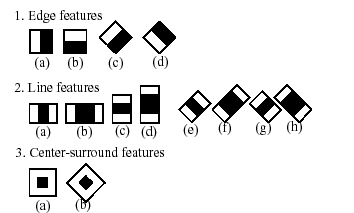
\includegraphics[width=0.5\textwidth]{pics/haarfeatures.png}

The feature used in a particular classifier is specified by its shape (1a, 2b etc.), position within the region of interest and the scale (this scale is not the same as the scale used at the detection stage, though these two scales are multiplied). For example, in case of the third line feature (2c) the response is calculated as the difference between the sum of image pixels under the rectangle covering the whole feature (including the two white stripes and the black stripe in the middle) and the sum of the image pixels under the black stripe multiplied by 3 in order to compensate for the differences in the size of areas. The sums of pixel values over a rectangular regions are calculated rapidly using integral images (see below and \cross{Integral} description).

To see the object detector at work, have a look at HaarFaceDetect demo.

The following reference is for the detection part only. There
is a separate application called \texttt{haartraining} that can
train a cascade of boosted classifiers from a set of samples. See
\texttt{opencv/apps/haartraining} for details.

\cvfunc{CvHaarFeature, CvHaarClassifier, CvHaarStageClassifier, CvHaarClassifierCascade}
\label{CvHaarFeature}
\label{CvHaarClassifier}
\label{CvHaarStageClassifier}
\label{CvHaarClassifierCascade}

Boosted Haar classifier structures

\begin{lstlisting}
#define CV_HAAR_FEATURE_MAX  3

/* a haar feature consists of 2-3 rectangles with appropriate weights */
typedef struct CvHaarFeature
{
    int  tilted;  /* 0 means up-right feature, 1 means 45--rotated feature */

    /* 2-3 rectangles with weights of opposite signs and
       with absolute values inversely proportional to the areas of the rectangles.
       if rect[2].weight !=0, then
       the feature consists of 3 rectangles, otherwise it consists of 2 */
    struct
    {
        CvRect r;
        float weight;
    } rect[CV_HAAR_FEATURE_MAX];
}
CvHaarFeature;

/* a single tree classifier (stump in the simplest case) that returns the response for the feature
   at the particular image location (i.e. pixel sum over subrectangles of the window) and gives out
   a value depending on the responce */
typedef struct CvHaarClassifier
{
    int count;  /* number of nodes in the decision tree */

    /* these are "parallel" arrays. Every index \texttt{i}
       corresponds to a node of the decision tree (root has 0-th index).

       left[i] - index of the left child (or negated index if the left child is a leaf)
       right[i] - index of the right child (or negated index if the right child is a leaf)
       threshold[i] - branch threshold. if feature responce is <= threshold, left branch
                      is chosen, otherwise right branch is chosed.
       alpha[i] - output value correponding to the leaf. */
    CvHaarFeature* haar_feature;
    float* threshold;
    int* left;
    int* right;
    float* alpha;
}
CvHaarClassifier;

/* a boosted battery of classifiers(=stage classifier):
   the stage classifier returns 1
   if the sum of the classifiers' responces
   is greater than \texttt{threshold} and 0 otherwise */
typedef struct CvHaarStageClassifier
{
    int  count;  /* number of classifiers in the battery */
    float threshold; /* threshold for the boosted classifier */
    CvHaarClassifier* classifier; /* array of classifiers */

    /* these fields are used for organizing trees of stage classifiers,
       rather than just stright cascades */
    int next;
    int child;
    int parent;
}
CvHaarStageClassifier;

typedef struct CvHidHaarClassifierCascade CvHidHaarClassifierCascade;

/* cascade or tree of stage classifiers */
typedef struct CvHaarClassifierCascade
{
    int  flags; /* signature */
    int  count; /* number of stages */
    CvSize orig_window_size; /* original object size (the cascade is trained for) */

    /* these two parameters are set by cvSetImagesForHaarClassifierCascade */
    CvSize real_window_size; /* current object size */
    double scale; /* current scale */
    CvHaarStageClassifier* stage_classifier; /* array of stage classifiers */
    CvHidHaarClassifierCascade* hid_cascade; /* hidden optimized representation of the cascade,
                                                created by cvSetImagesForHaarClassifierCascade */
}
CvHaarClassifierCascade;
\end{lstlisting}

All the structures are used for representing a cascaded of boosted Haar classifiers. The cascade has the following hierarchical structure:

\begin{verbatim}
    Cascade:
        Stage,,1,,:
            Classifier,,11,,:
                Feature,,11,,
            Classifier,,12,,:
                Feature,,12,,
            ...
        Stage,,2,,:
            Classifier,,21,,:
                Feature,,21,,
            ...
        ...
\end{verbatim}

The whole hierarchy can be constructed manually or loaded from a file or an embedded base using function \cross{LoadHaarClassifierCascade}.


\cvfunc{LoadHaarClassifierCascade}\label{LoadHaarClassifierCascade}

Loads a trained cascade classifier from file or the classifier database embedded in OpenCV

\cvexp{
CvHaarClassifierCascade* cvLoadHaarClassifierCascade( \par const char* directory,\par CvSize orig\_window\_size );
}{CPP}{PYTHON}

\begin{description}
\cvarg{directory}{Name of directory containing the description of a trained cascade classifier}
\cvarg{orig\_window\_size}{Original size of objects the cascade has been trained on. Note that it is not stored in the cascade and therefore must be specified separately}
\end{description}

The function \texttt{cvLoadHaarClassifierCascade} loads a trained cascade
of haar classifiers from a file or the classifier database embedded in
OpenCV. The base can be trained using \texttt{haartraining} application
(see opencv/apps/haartraining for details).

\textbf{The function is obsolete}. Nowadays object detection classifiers are stored in XML or YAML files, rather than in directories. To load cascade from a file, use cvLoad function.

\cvfunc{ReleaseHaarClassifierCascade}\label{ReleaseHaarClassifierCascade}

Releases haar classifier cascade

\cvexp{
void cvReleaseHaarClassifierCascade( \par CvHaarClassifierCascade** cascade );
}{CPP}{PYTHON}

\begin{description}
\cvarg{cascade}{Double pointer to the released cascade. The pointer is cleared by the function}
\end{description}

The function \texttt{cvReleaseHaarClassifierCascade} deallocates the cascade that has been created manually or loaded using \cross{LoadHaarClassifierCascade} or \cross{Load}.

\cvfunc{HaarDetectObjects}\label{HaarDetectObjects}

Detects objects in the image

\begin{lstlisting}
typedef struct CvAvgComp
{
    CvRect rect; /* bounding rectangle for the object (average rectangle of a group) */
    int neighbors; /* number of neighbor rectangles in the group */
}
CvAvgComp;
\end{lstlisting}

\cvexp{
CvSeq* cvHaarDetectObjects( \par const CvArr* image,\par CvHaarClassifierCascade* cascade,\par CvMemStorage* storage,\par double scale\_factor=1.1,\par int min\_neighbors=3,\par int flags=0,\par CvSize min\_size=cvSize(0,\par0) );
}{CPP}{HaarDetectObjects(image,cascade,storage,scale\_factor=1.1,min\_neighbors=3,flags=0,min\_size=(0,0))-> detected\_objects}

\begin{description}
\cvarg{image}{Image to detect objects in}
\cvarg{cascade}{Haar classifier cascade in internal representation}
\cvarg{storage}{Memory storage to store the resultant sequence of the object candidate rectangles}
\cvarg{scale\_factor}{The factor by which the search window is scaled between the subsequent scans, for example, 1.1 means increasing window by 10\% }
\cvarg{min\_neighbors}{Minimum number (minus 1) of neighbor rectangles that makes up an object. All the groups of a smaller number of rectangles than \texttt{min\_neighbors}-1 are rejected. If \texttt{min\_neighbors} is 0, the function does not any grouping at all and returns all the detected candidate rectangles, which may be useful if the user wants to apply a customized grouping procedure}
\cvarg{flags}{Mode of operation. Currently the only flag that may be specified is \texttt{CV\_HAAR\_DO\_CANNY\_PRUNING}. If it is set, the function uses Canny edge detector to reject some image regions that contain too few or too much edges and thus can not contain the searched object. The particular threshold values are tuned for face detection and in this case the pruning speeds up the processing}
\cvarg{min\_size}{Minimum window size. By default, it is set to the size of samples the classifier has been trained on ($\sim 20\times 20$ for face detection)}
\end{description}

The function \texttt{cvHaarDetectObjects} finds rectangular regions in the given image that are likely to contain objects the cascade has been trained for and returns those regions as a sequence of rectangles. The function scans the image several times at different scales (see \cross{SetImagesForHaarClassifierCascade}). Each time it considers overlapping regions in the image and applies the classifiers to the regions using \cross{RunHaarClassifierCascade}. It may also apply some heuristics to reduce number of analyzed regions, such as Canny prunning. After it has proceeded and collected the candidate rectangles (regions that passed the classifier cascade), it groups them and returns a sequence of average rectangles for each large enough group. The default parameters (\texttt{scale\_factor} =1.1, \texttt{min\_neighbors} =3, \texttt{flags} =0) are tuned for accurate yet slow object detection. For a faster operation on real video images the settings are: \texttt{scale\_factor} =1.2, \texttt{min\_neighbors} =2, \texttt{flags} =\texttt{CV\_HAAR\_DO\_CANNY\_PRUNING}, \texttt{min\_size} =\textit{minimum possible face size} (for example, $\sim$ 1/4 to 1/16 of the image area in case of video conferencing).

% ===== Example. Using cascade of Haar classifiers to find objects (e.g. faces). =====
\begin{lstlisting}
#include "cv.h"
#include "highgui.h"

CvHaarClassifierCascade* load_object_detector( const char* cascade_path )
{
    return (CvHaarClassifierCascade*)cvLoad( cascade_path );
}

void detect_and_draw_objects( IplImage* image,
                              CvHaarClassifierCascade* cascade,
                              int do_pyramids )
{
    IplImage* small_image = image;
    CvMemStorage* storage = cvCreateMemStorage(0);
    CvSeq* faces;
    int i, scale = 1;

    /* if the flag is specified, down-scale the input image to get a
       performance boost w/o loosing quality (perhaps) */
    if( do_pyramids )
    {
        small_image = cvCreateImage( cvSize(image->width/2,image->height/2), IPL_DEPTH_8U, 3 );
        cvPyrDown( image, small_image, CV_GAUSSIAN_5x5 );
        scale = 2;
    }

    /* use the fastest variant */
    faces = cvHaarDetectObjects( small_image, cascade, storage, 1.2, 2, CV_HAAR_DO_CANNY_PRUNING );

    /* draw all the rectangles */
    for( i = 0; i < faces->total; i++ )
    {
        /* extract the rectanlges only */
        CvRect face_rect = *(CvRect*)cvGetSeqElem( faces, i, 0 );
        cvRectangle( image, cvPoint(face_rect.x*scale,face_rect.y*scale),
                     cvPoint((face_rect.x+face_rect.width)*scale,
                             (face_rect.y+face_rect.height)*scale),
                     CV_RGB(255,0,0), 3 );
    }

    if( small_image != image )
        cvReleaseImage( &small_image );
    cvReleaseMemStorage( &storage );
}

/* takes image filename and cascade path from the command line */
int main( int argc, char** argv )
{
    IplImage* image;
    if( argc==3 && (image = cvLoadImage( argv[1], 1 )) != 0 )
    {
        CvHaarClassifierCascade* cascade = load_object_detector(argv[2]);
        detect_and_draw_objects( image, cascade, 1 );
        cvNamedWindow( "test", 0 );
        cvShowImage( "test", image );
        cvWaitKey(0);
        cvReleaseHaarClassifierCascade( &cascade );
        cvReleaseImage( &image );
    }

    return 0;
}
\end{lstlisting}

\cvfunc{SetImagesForHaarClassifierCascade}\label{SetImagesForHaarClassifierCascade}

Assigns images to the hidden cascade

\cvexp{
void cvSetImagesForHaarClassifierCascade( \par CvHaarClassifierCascade* cascade,\par const CvArr* sum,\par const CvArr* sqsum,\par const CvArr* tilted\_sum,\par double scale );
}{CPP}{PYTHON}

\begin{description}
\cvarg{cascade}{Hidden Haar classifier cascade, created by \cross{CreateHidHaarClassifierCascade}}
\cvarg{sum}{Integral (sum) single-channel image of 32-bit integer format. This image as well as the two subsequent images are used for fast feature evaluation and brightness/contrast normalization. They all can be retrieved from input 8-bit or floating point single-channel image using The function \cross{Integral}}
\cvarg{sqsum}{Square sum single-channel image of 64-bit floating-point format}
\cvarg{tilted\_sum}{Tilted sum single-channel image of 32-bit integer format}
\cvarg{scale}{Window scale for the cascade. If \texttt{scale} =1, original window size is used (objects of that size are searched) - the same size as specified in \cross{LoadHaarClassifierCascade} (24x24 in case of \texttt{default\_face\_cascade}), if \texttt{scale} =2, a two times larger window is used (48x48 in case of default face cascade). While this will speed-up search about four times, faces smaller than 48x48 cannot be detected}
\end{description}

The function \texttt{cvSetImagesForHaarClassifierCascade} assigns images and/or window scale to the hidden classifier cascade. If image pointers are NULL, the previously set images are used further (i.e. NULLs mean "do not change images"). Scale parameter has no such a "protection" value, but the previous value can be retrieved by \cross{GetHaarClassifierCascadeScale} function and reused again. The function is used to prepare cascade for detecting object of the particular size in the particular image. The function is called internally by \cross{HaarDetectObjects}, but it can be called by user if there is a need in using lower-level function \cross{RunHaarClassifierCascade}.

\cvfunc{RunHaarClassifierCascade}\label{RunHaarClassifierCascade}

Runs cascade of boosted classifier at given image location

\cvexp{
int cvRunHaarClassifierCascade( \par CvHaarClassifierCascade* cascade,\par CvPoint pt,\par int start\_stage=0 );
}{CPP}{PYTHON}

\begin{description}
\cvarg{cascade}{Haar classifier cascade}
\cvarg{pt}{Top-left corner of the analyzed region. Size of the region is a original window size scaled by the currenly set scale. The current window size may be retrieved using \cross{GetHaarClassifierCascadeWindowSize} function}
\cvarg{start\_stage}{Initial zero-based index of the cascade stage to start from. The function assumes that all the previous stages are passed. This feature is used internally by \cross{HaarDetectObjects} for better processor cache utilization}
\end{description}

The function \texttt{cvRunHaarHaarClassifierCascade} runs Haar classifier
cascade at a single image location. Before using this function the
integral images and the appropriate scale (window size) should be set
using \cross{SetImagesForHaarClassifierCascade}. The function returns
positive value if the analyzed rectangle passed all the classifier stages
(it is a candidate) and zero or negative value otherwise.

\section{Camera Calibration and 3D Reconstruction}

\subsection{Pinhole Camera Model, Distortion}

The functions in this section use so-called pinhole camera model. That
is, a scene view is formed by projecting 3D points into the image plane
using perspective transformation.

\[
s \quad m' = A [R|t] M'
\]

or

\[
s \vecthree{u}{v}{1} = \vecthreethree
{fx}{0}{cx}
{0}{fy}{cy}
{0}{0}{1}
\begin{bmatrix}
 r_{11} & r_{12} & r{13} & t_1 \\
 r_{21} & r_{22} & r{23} & t_2 \\
 r_{31} & r_{32} & r{33} & t_3
\end{bmatrix}
\begin{bmatrix}X\\Y\\Z\\1 \end{bmatrix}
\]

Where $(X, Y, Z)$ are coordinates of a 3D point in the world
coordinate space, $(u, v)$ are coordinates of point projection
in pixels. $A$ is called a camera matrix, or matrix of
intrinsic parameters. $(cx, cy)$ is a principal point (that is
usually at the image center), and $fx, fy$ are focal lengths
expressed in pixel-related units. Thus, if an image from camera is
up-sampled/down-sampled by some factor, all these parameters should
be scaled (multiplied/divided, respectively) by the same factor. The
matrix of intrinsic parameters does not depend on the scene viewed and,
once estimated, can be re-used (as long as the focal length is fixed (in
case of zoom lens)). The joint rotation-translation matrix $[R|t]$
is called a matrix of extrinsic parameters. It is used to describe the
camera motion around a static scene, or vice versa, rigid motion of an
object in front of still camera. That is, $[R|t]$ translates
coordinates of a point $(X, Y, Z)$ to some coordinate system,
fixed with respect to the camera. The transformation above is equivalent
to the following (when $z \ne 0$):

\[
\begin{array}{l}
\vecthree{x}{y}{z} = R \vecthree{X}{Y}{Z} + t\\
x' = x/z\\
y' = y/z\\
u = fx*x' + cx\\
v = fy*y' + cy
\end{array}
\]

Real lens usually have some distortion, which major components are
radial distorion and slight tangential distortion. So, the above model
is extended as:

\[
\begin{array}{l}
\vecthree{x}{y}{z} = R \vecthree{X}{Y}{Z} + t\\
x' = x/z\\
y' = y/z\\
x'' = x' (1 + k_1 r^2 + k_2 r^4 + k_3 r^6) + 2 p_1 x' y' + p_2(r^2 + 2 x'^2) \\
y'' = y' (1 + k_1 r^2 + k_2 r^4 + k_3 r^6) + p_1 (r^2 + 2 y'^2) + 2 p_2 x' y' \\
\text{where} \quad r^2 = x'^2 + y'^2 \\
u = fx*x'' + cx\\
v = fy*y'' + cy
\end{array}
\]

$k_1$, $k_2$, $k_3$ are radial distortion coefficients, $p_1$, $p_2$ are tangential distortion coefficients.
Higher-order coefficients are not considered in OpenCV.
The distortion coefficients also do not depend on the scene viewed, thus they are intrinsic camera parameters.
\emph{And they remain the same regardless of the captured image resolution.}
That is, if, for example, a camera has been calibrated on images of $320
\times 240$ resolution, absolutely the same distortion coefficients can
be used for images of $640 \times 480$ resolution from the same camera (while $fx$,
$fy$, $cx$ and $cy$ need to be scaled appropriately).

The functions below use the above model to

\begin{itemize}
 \item Project 3D points to the image plane given intrinsic and extrinsic parameters
 \item Compute extrinsic parameters given intrinsic parameters, a few 3D points and their projections.
 \item Estimate intrinsic and extrinsic camera parameters from several views of a known calibration pattern (i.e. every view is described by several 3D-2D point correspodences).
\end{itemize}

\subsection{Camera Calibration}

\cvfunc{ProjectPoints2}\label{ProjectPoints2}

Projects 3D points to image plane

\cvexp{
void cvProjectPoints2( \par const CvMat* object\_points,\par const CvMat* rotation\_vector,\par const CvMat* translation\_vector,\par const CvMat* intrinsic\_matrix,\par const CvMat* distortion\_coeffs,\par CvMat* image\_points,\par CvMat* dpdrot=NULL,\par CvMat* dpdt=NULL,\par CvMat* dpdf=NULL,\par CvMat* dpdc=NULL,\par CvMat* dpddist=NULL );
}{CPP}{ProjectPoints2(object\_points,rotation\_vector,translation\_vector,intrinsic\_matrix,distortion\_coeffs, image\_points,dpdrot=NULL,dpdt=NULL,dpdf=NULL,dpdc=NULL,dpddist=NULL)-> None}

\begin{description}
\cvarg{object\_points}{The array of object points, 3xN or Nx3, where N is the number of points in the view}
\cvarg{rotation\_vector}{The rotation vector, 1x3 or 3x1}
\cvarg{translation\_vector}{The translation vector, 1x3 or 3x1}
\cvarg{intrinsic\_matrix}{The camera matrix $A = \vecthreethree{fx}{0}{cx}{0}{fy}{cy}{0}{0}{1} $}
\cvarg{distortion\_coeffs}{The vector of distortion coefficients, 4x1 or 1x4 $k_1, k_2, k_3, k_4$. If it is \texttt{NULL}, all distortion coefficients are considered 0's}
\cvarg{image\_points}{The output array of image points, 2xN or Nx2, where N is the total number of points in the view}
\cvarg{dpdrot}{Optional Nx3 matrix of derivatives of image points with respect to components of the rotation vector}
\cvarg{dpdt}{Optional Nx3 matrix of derivatives of image points w.r.t. components of the translation vector}
\cvarg{dpdf}{Optional Nx2 matrix of derivatives of image points w.r.t. $fx$ and $fy$}
\cvarg{dpdc}{Optional Nx2 matrix of derivatives of image points w.r.t. $cx$ and $cy$}
\cvarg{dpddist}{Optional Nx4 matrix of derivatives of image points w.r.t. distortion coefficients}
\end{description}

The function \texttt{cvProjectPoints2} computes projections of 3D
points to the image plane given intrinsic and extrinsic camera
parameters. Optionally, the function computes jacobians - matrices
of partial derivatives of image points as functions of all the
input parameters w.r.t. the particular parameters, intrinsic and/or
extrinsic. The jacobians are used during the global optimization
in \cross{CalibrateCamera2} and
\cross{FindExtrinsicCameraParams2}. The
function itself is also used to compute back-projection error for with
current intrinsic and extrinsic parameters.

Note, that with intrinsic and/or extrinsic parameters set to special
values, the function can be used to compute just extrinsic transformation
or just intrinsic transformation (i.e. distortion of a sparse set
of points).

\cvfunc{FindHomography}\label{FindHomography}

Finds perspective transformation between two planes

\cvexp{
void cvFindHomography( \par const CvMat* src\_points,\par const CvMat* dst\_points,\par CvMat* homography \par
int method=0, \par double ransacReprojThreshold=0, \par CvMat* mask=NULL);
}{CPP}{FindHomography(src\_points,dst\_points)-> homography}

\begin{description}
\cvarg{src\_points}{Point coordinates in the original plane, 2xN, Nx2, 3xN or Nx3 array (the latter two are for representation in homogenious coordinates), where N is the number of points}
\cvarg{dst\_points}{Point coordinates in the destination plane, 2xN, Nx2, 3xN or Nx3 array (the latter two are for representation in homogenious coordinates)}
\cvarg{homography}{Output 3x3 homography matrix}
\cvarg{method}{ The method used to computed homography matrix. One of:
\begin{description}
\cvarg{0}{regular method using all the point pairs}
\cvarg{CV\_RANSAC}{RANSAC-based robust method}
\cvarg{CV\_LMEDS}{Least-Median robust method}
\end{description}}
\cvarg{ransacReprojThreshold}{The maximum allowed reprojection error to treat a point pair as an inlier. The parameter is only used in RANSAC-based homography estimation. E.g. if \texttt{dst\_points} coordinates are measured in pixels with pixel-accurate precision, it makes sense to set this parameter somewhere in the range $1...3$. }
\cvarg{mask}{The optional output mask set by a robust method (\texttt{CV\_RANSAC} or \texttt{CV\_LMEDS}).}
\end{description}

The function \texttt{cvFindHomography} finds perspective transformation $H$ between the source and the destination planes:

\[
s_i \vecthree{x'_i}{y'_i}{1} \sim H \vecthree{x_i}{y_i}{1}
\]

So that the back-projection error is minimized:

\[
\sum_i
\left( x'_i-\frac{h_{11} x_i + h_{12} y_i + h_{13}}{h_{31} x_i + h_{32} y_i + h_{33}} \right)^2+
\left( y'_i-\frac{h_{21} x_i + h_{22} y_i + h_{23}}{h_{31} x_i + h_{32} y_i + h_{33}} \right)^2
\]

If the parameter method is set to the default value 0, the function
uses all the point pairs and estimates the best suitable homography
matrix. However, if there can not all the points pairs ($src\_points_i$,
$dst\_points_i$) fit the rigid perspective transformation (i.e. there
can be outliers), it is still possible to estimate the correct
transformation using one of the robust methods available. Both
methods, \texttt{CV\_RANSAC} and \texttt{CV\_LMEDS}, try many different random subsets
of the corresponding point pairs (of 5 pairs each), estimate
homography matrix using this subset using simple least-square
algorithm and then compute quality/goodness of the computed homography
(which is the number of inliers for RANSAC or the median reprojection
error for LMeDs). The best subset is then used to produce the initial
estimate of the homography matrix and the mask of inliers/outliers.

Regardless of the method, robust or not, the computed homography
matrix is refined further (using inliers only in case of a robust
method) with Levenberg-Marquardt method in order to reduce the
reprojection error even more.

The method \texttt{CV\_RANSAC} can handle practically any ratio of outliers,
but it needs the threshold to distinguish inliers from outliers.
The method \texttt{CV\_LMEDS} does not need any threshold, but it works
correctly only when there are more than 50\% of inliers. Finally,
if you are sure in the computed features and there can be only some
small noise, but no outliers, the default method could be the best
choice.

The function is used to find initial intrinsic and extrinsic matrices.
Homography matrix is determined up to a scale, thus it is normalized
to make $h_{33} =1$.

\cvfunc{CalibrateCamera2}\label{CalibrateCamera2}

Finds intrinsic and extrinsic camera parameters using calibration pattern

\cvexp{
void cvCalibrateCamera2( \par const CvMat* object\_points,\par const CvMat* image\_points,\par const CvMat* point\_counts,\par CvSize image\_size,\par CvMat* intrinsic\_matrix,\par CvMat* distortion\_coeffs,\par CvMat* rotation\_vectors=NULL,\par CvMat* translation\_vectors=NULL,\par int flags=0 );
}{CPP}{CalibrateCamera2(object\_points,image\_points,point\_counts,image\_size,intrinsic\_matrix,distortion\_coeffs,rotation\_vectors,translation\_vectors,flags=0)-> None}

\begin{description}
\cvarg{object\_points}{The joint matrix of object points, 3xN or Nx3, where N is the total number of points in all views}
\cvarg{image\_points}{The joint matrix of corresponding image points, 2xN or Nx2, where N is the total number of points in all views}
\cvarg{point\_counts}{Vector containing numbers of points in each particular view, 1xM or Mx1, where M is the number of a scene views}
\cvarg{image\_size}{Size of the image, used only to initialize intrinsic camera matrix}
\cvarg{intrinsic\_matrix}{The output camera matrix $A = \vecthreethree{fx}{0}{cx}{0}{fy}{cy}{0}{0}{1} $. If \texttt{CV\_CALIB\_USE\_INTRINSIC\_GUESS} and/or \texttt{CV\_CALIB\_FIX\_ASPECT\_RATION} are specified, some or all of \texttt{fx, fy, cx, cy} must be initialized}
\cvarg{distortion\_coeffs}{The output 4x1 or 1x4 vector of distortion coefficients $k_1, k_2, k_3, k_4$}
\cvarg{rotation\_vectors}{The output 3xM or Mx3 array of rotation vectors (compact representation of rotation matrices, \cross{Rodrigues2})}
\cvarg{translation\_vectors}{The output 3xM or Mx3 array of translation vectors}
\cvarg{flags}{Different flags, may be 0 or combination of the following values:
\begin{description}
\cvarg{CV\_CALIB\_USE\_INTRINSIC\_GUESS}{\texttt{intrinsic\_matrix} contains valid initial values of \texttt{fx, fy, cx, cy} that are optimized further. Otherwise, \texttt{(cx, cy)} is initially set to the image center (\texttt{image\_size} is used here), and focal distances are computed in some least-squares fashion. Note, that if intrinsic parameters are known, there is no need to use this function. Use \cross{FindExtrinsicCameraParams2} instead.}
\cvarg{CV\_CALIB\_FIX\_PRINCIPAL\_POINT}{The principal point is not changed during the global optimization, it stays at the center and at the other location specified (when \texttt{CV\_CALIB\_USE\_INTRINSIC\_GUESS} is set as well)}
\cvarg{CV\_CALIB\_FIX\_ASPECT\_RATIO}{The optimization procedure consider only one of \texttt{fx} and \texttt{fy} as independent variable and keeps the aspect ratio \texttt{fx/fy} the same as it was set initially in \texttt{intrinsic\_matrix}. In this case the actual initial values of \texttt{(fx, fy)} are either taken from the matrix (when \texttt{CV\_CALIB\_USE\_INTRINSIC\_GUESS} is set) or estimated somehow (in the latter case \texttt{fx, fy} may be set to arbitrary values, only their ratio is used).}
\cvarg{CV\_CALIB\_ZERO\_TANGENT\_DIST}{Tangential distortion coefficients are set to zeros and do not change during the optimization.}}
\end{description}
\end{description}

The function \texttt{cvCalibrateCamera2} estimates intrinsic camera
parameters and extrinsic parameters for each of the views. The
coordinates of 3D object points and their correspondent 2D projections
in each view must be specified. That may be achieved by using an
object with known geometry and easily detectable feature points.
Such an object is called calibration rig or calibration pattern,
and OpenCV has built-in support for a chessboard as a calibration
rig (see \cross{FindChessboardCornerGuesses}). Currently, initialization
of inrtrinsic parameters (when \texttt{CV\_CALIB\_USE\_INTRINSIC\_GUESS}
is not set) is only implemented for planar calibration rigs
(z-coordinates of object points must be all 0's or all 1's). 3D
rigs can still be used as long as initial \texttt{intrinsic\_matrix}
is provided. After the initial values of intrinsic and extrinsic
parameters are computed, they are optimized to minimize the total
back-projection error - the sum of squared differences between the
actual coordinates of image points and the ones computed using
\cross{ProjectPoints2}.

Note: if you're using a non-square (=non-NxN) grid and
\cross{FindChessboardCorners} for calibration, and cvCalibrateCamera2 returns
bad values (i.e. zero distortion coefficients, an image center of
(w/2-0.5,h/2-0.5), and / or large differences between $fx$ and $fy$ (ratios of
10:1 or more)), then you've probaby  used pattern\_size=cvSize(rows,cols),
but should use pattern\_size=cvSize(cols,rows) in \cross{FindChessboardCorners}.

\cvfunc{FindExtrinsicCameraParams2}\label{FindExtrinsicCameraParams2}

Finds extrinsic camera parameters for particular view

\cvexp{
void cvFindExtrinsicCameraParams2( \par const CvMat* object\_points,\par const CvMat* image\_points,\par const CvMat* intrinsic\_matrix,\par const CvMat* distortion\_coeffs,\par CvMat* rotation\_vector,\par CvMat* translation\_vector );
}{CPP}{FindExtrinsicCameraParams2(object\_points,image\_points,intrinsic\_matrix,distortion\_coeffs,rotation\_vector,translation\_vector)-> None}

\begin{description}
\cvarg{object\_points}{The array of object points, 3xN or Nx3, where N is the number of points in the view}
\cvarg{image\_points}{The array of corresponding image points, 2xN or Nx2, where N is the number of points in the view}
\cvarg{intrinsic\_matrix}{The output camera matrix $A = \vecthreethree{fx}{0}{cx}{0}{fy}{cy}{0}{0}{1} $}
\cvarg{distortion\_coeffs}{The output 4x1 or 1x4 vector of distortion coefficients $k_1, k_2, k_3, k_4$. If it is NULL, all distortion coefficients are considered 0's}
\cvarg{rotation\_vector}{The output 3x1 or 1x3 rotation vector (compact representation of a rotation matrix, cvRodrigues2}
\cvarg{translation\_vector}{The output 3x1 or 1x3 translation vector}
\end{description}

The function \texttt{cvFindExtrinsicCameraParams2} estimates extrinsic camera parameters using known intrinsic parameters and extrinsic parameters for each view. The coordinates of 3D object points and their correspondent 2D projections must be specified. This function also minimizes back-projection error.

\cvfunc{StereoCalibrate}

Calibrates stereo camera.

\cvexp{

void cvStereoCalibrate( \par const CvMat* object\_points, \par const CvMat* image\_points1,
                        \par const CvMat* image\_points2, \par const CvMat* point\_counts,
                        \par CvMat* camera\_matrix1, \par CvMat* dist\_coeffs1,
                        \par CvMat* camera\_matrix2, \par CvMat* dist\_coeffs2,
                       \par CvSize image\_size, \par CvMat* R, \par CvMat* T,
                        \par CvMat* E=0, \par CvMat* F=0,
                        \par CvTermCriteria term\_crit=cvTermCriteria(
                               \par CV\_TERMCRIT\_ITER+CV\_TERMCRIT\_EPS,30,1e-6),
                        \par int flags=CV\_CALIB\_FIX\_INTRINSIC );

}{CPP}{StereoCalibrate(\par object\_points,\par image\_points1,\par image\_points2,\par point\_counts,\par camera\_matrix1,\par dist\_coeffs1,\par camera\_matrix2,\par dist\_coeffs2,\par image\_size,\par R,\par T,\par E=NULL,\par F=NULL,\par term\_crit=cvTermCriteria(CV\_TERMCRIT\_ITER+CV\_TERMCRIT\_EPS,30,1e-6),\par flags=CV\_CALIB\_FIX\_INTRINSIC)-> None}

\begin{description}
\cvarg{object\_points}{The joint matrix of object points, 3xN or Nx3, where N is the total number of points in all views.}
\cvarg{image\_points1}{The joint matrix of corresponding image points in the views from the 1st camera, 2xN or Nx2, where N is the total number of points in all views.}
\cvarg{image\_points2}{The joint matrix of corresponding image points in the views from the 2nd camera, 2xN or Nx2, where N is the total number of points in all views.}
\cvarg{point\_counts}{Vector containing numbers of points in each view, 1xM or Mx1, where M is the number of views.}
\cvarg{camera\_matrix1, camera\_matrix2}{The input/output camera matrices [${fx}_k 0 {cx}_k; 0 {fy}_k {cy}_k; 0 0 1$]. If \texttt{CV\_CALIB\_USE\_INTRINSIC\_GUESS} or \texttt{CV\_CALIB\_FIX\_ASPECT\_RATIO} are specified, some or all of the elements of the matrices must be initialized.}
\cvarg{dist\_coeffs1, dist\_coeffs2}{The input/output vectors of distortion coefficients for each camera, \href{\#Pinhole Camera Model, Distortion}{4x1, 1x4, 5x1 or 1x5.}}
\cvarg{image\_size}{Size of the image, used only to initialize intrinsic camera matrix.} 
\cvarg{R}{The rotation matrix between the 1st and the 2nd cameras' coordinate systems.}
\cvarg{T}{The translation vector between the cameras' coordinate systems.}
\cvarg{E}{The optional output essential matrix.}
\cvarg{F}{The optional output fundamental matrix.}
\cvarg{term\_crit}{Termination criteria for the iterative optimiziation algorithm.}
\cvarg{flags}{Different flags, may be 0 or combination of the following values:
\begin{description}
\cvarg{CV\_CALIB\_FIX\_INTRINSIC}{If it is set, \texttt{camera\_matrix1,2}, as well as \texttt{dist\_coeffs1,2} are fixed, so that only extrinsic parameters are optimized.}
\cvarg{CV\_CALIB\_USE\_INTRINSIC\_GUESS}{The flag allows the function to optimize some or all of the intrinsic parameters, depending on the other flags, but the initial values are provided by the user.}
\cvarg{CV\_CALIB\_FIX\_PRINCIPAL\_POINT}{The principal points are fixed during the optimization.}
\cvarg{CV\_CALIB\_FIX\_FOCAL\_LENGTH}{${fx}_k$ and ${fy}_k$ are fixed.}
\cvarg{CV\_CALIB\_FIX\_ASPECT\_RATIO}{${fy}_k$ is optimized, but the ratio ${fx}_k/{fy}_k$ is fixed.}
\cvarg{CV\_CALIB\_SAME\_FOCAL\_LENGTH}{Enforces ${fx}_0={fx}_1$ and ${fy}_0={fy}_1$. \texttt{CV\_CALIB\_ZERO\_TANGENT\_DIST} - Tangential distortion coefficients for each camera are set to zeros and fixed there.}
\cvarg{CV\_CALIB\_FIX\_K1}{The 0-th distortion coefficients (k1) are fixed.}
\cvarg{CV\_CALIB\_FIX\_K2}{The 1-st distortion coefficients (k2) are fixed.}
\cvarg{CV\_CALIB\_FIX\_K3}{The 4-th distortion coefficients (k3) are fixed.}
\end{description}}
\end{description}

The function \texttt{cvStereoCalibrate} estimates transformation between the 2 cameras making a stereo pair. If we have a stereo camera, where the relative position and orientatation of the 2 cameras is fixed, and if we computed poses of an object relative to the fist camera and to the second camera, (R1, T1) and (R2, T2), respectively (that can be done with \cross{cvFindExtrinsicCameraParams2}), obviously, those poses will relate to each other, i.e. given ($R_1$, $T_1$) it should be possible to compute ($R_2$, $T_2$) - we only need to know the position and orientation of the 2nd camera relative to the 1st camera. That's what the described function does. It computes ($R$, $T$) such that:

\[
R_2=R*R_1
T_2=R*T_1 + T,
\]

Optionally, it computes the essential matrix E:

\[
E=
\vecthreethree
{0}{-T_2}{T_1}
{T_2}{0}{-T_0}
{-T_1}{T_0}{0}
*R
\]

where $T_i$ are components of the translation vector $T$: $T=[T_0, T_1, T_2]^T$. And also the function can compute the fundamental matrix F:

$F = inv(camera\_matrix2)^T*E*inv(camera\_matrix1)$

Besides the stereo-related information, the function can also perform full calibration of each of the 2 cameras. However, because of the high dimensionality of the parameter space and noise in the input data the function can diverge from the correct solution. Thus, if intrinsic parameters can be estimated with high accuracy for each of the cameras individually (e.g. using \cross{cvCalibrateCamera2}), it is recommended to do so and then pass \texttt{CV\_CALIB\_FIX\_INTRINSIC} flag to the function along with the computed intrinsic parameters. Otherwise, if all the parameters are estimated at once, it makes sense to restrict some parameters, e.g. pass \texttt{CV\_CALIB\_SAME\_FOCAL\_LENGTH} and \texttt{CV\_CALIB\_ZERO\_TANGENT\_DIST} flags, which are usually reasonable assumptions. 

\cvfunc{StereoRectify}

Computes rectification transform for stereo camera.

\cvexp{

void cvStereoRectify( \par const CvMat* camera\_matrix1, \par const CvMat* camera\_matrix2,
                      \par const CvMat* dist\_coeffs1, \par const CvMat* dist\_coeffs2,
                      \par CvSize image\_size, \par const CvMat* R, \par const CvMat* T,
                      \par CvMat* R1, \par CvMat* R2, \par CvMat* P1, \par CvMat* P2,
                      \par CvMat* Q=0, \par int flags=CV\_CALIB\_ZERO\_DISPARITY );

}{CPP}{StereoRectify(\par camera\_matrix1,\par camera\_matrix2,\par dist\_coeffs1,\par dist\_coeffs2,\par image\_size,\par R,\par T,\par R1,\par R2,\par P1,\par P2,\par Q=NULL,\par flags=CV\_CALIB\_ZERO\_DISPARITY)-> None}

\begin{description}
\cvarg{camera\_matrix1, camera\_matrix2}{The camera matrices [${fx}_k$ 0 ${cx}_k$; 0 ${fy}_k$ ${cy}_k$; 0 0 1].}
\cvarg{dist\_coeffs1, dist\_coeffs2}{The vectors of distortion coefficients for each camera, \href{\#Pinhole Camera Model, Distortion}{4x1, 1x4, 5x1 or 1x5.}}
\cvarg{image\_size}{Size of the image used for stereo calibration.}
\cvarg{R}{The rotation matrix between the 1st and the 2nd cameras' coordinate systems.}
\cvarg{T}{The translation vector between the cameras' coordinate systems.}
\cvarg{R1, R2}{3x3 Rectification transforms (rotation matrices) for the first and the second cameras, respectively.}
\cvarg{P1, P2}{3x4 Projection matrices in the new (rectified) coordinate systems.}
\cvarg{Q}{The optional output disparity-to-depth mapping matrix, 4x4, see \cross{cvReprojectImageTo3D}.}
\cvarg{flags}{The operation flags; may be 0 or \texttt{CV\_CALIB\_ZERO\_DISPARITY}. If the flag is set, the function makes the principal points of each camera have the same pixel coordinates in the rectified views. And if the flag is not set, the function can shift one of the image in horizontal or vertical direction (depending on the orientation of epipolar lines) in order to maximise the useful image area. }
\end{description}

The function \texttt{cvStereoRectify} computes the rotation matrices for each camera that (virtually) make both camera image planes the same plane. Consequently, that makes all the epipolar lines parallel and thus simplifies the dense stereo correspondence problem. On input the function takes the matrices computed by \cross{cvStereoCalibrate} and on output it gives 2 rotation matrices and also 2 projection matrices in the new coordinates. The function is normally called after \cross{cvStereoCalibrate} that computes both camera matrices, the distortion coefficients, R and T. The 2 cases are distinguished by the function: 

\begin{enumerate}
\item{Horizontal stereo, when 1st and 2nd camera views are shifted relative to each other mainly along the x axis (with possible small vertical shift). Then in the rectified images the corresponding epipolar lines in left and right cameras will be horizontal and have the same y-coordinate. P1 and P2 will look as: 

\[
P1=
\begin{array}{cccc}
f & 0 & cx1 & 0\\
0 & f & cy & 0\\
0 & 0 & 1 & 0
\end{array}
\]
\[
P2=
\begin{array}{cccc}
f & 0 & cx2 & Tx*f\\
0 & f & cy & 0\\
0 & 0 & 1 & 0
\end{array}
,
\]

where $T_x$ is horizontal shift between the cameras and cx1=cx2 if \texttt{CV\_CALIB\_ZERO\_DISPARITY} is set.}
\item{Vertical stereo, when 1st and 2nd camera views are shifted relative to each other mainly in vertical direction (and probably a bit in the horizontal direction too). Then the epipolar lines in the rectified images will be vertical and have the same x coordinate. P2 and P2 will look as:

\[
P1=
\begin{array}{cccc}
f & 0 & cx & 0\\
0 & f & cy1 & 0\\
0 & 0 & 1 & 0
\end{array}
\]
\[
P2=
\begin{array}{cccc}
f & 0 & cx & 0\\
0 & f & cy2 & Ty*f\\
0 & 0 & 1 & 0
\end{array}
,
\]

where $T_y$ is vertical shift between the cameras and cy1=cy2 if \texttt{CV\_CALIB\_ZERO\_DISPARITY} is set.}
\end{enumerate} 

As you can see, the first 3 columns of P1 and P2 will effectively be the new "rectified" camera matrices. 

\cvfunc{StereoRectifyUncalibrated}

Computes rectification transform for uncalibrated stereo camera.

\cvexp{

void cvStereoRectifyUncalibrated( \par const CvMat* points1, \par const CvMat* points2,
                                  \par const CvMat* F, \par CvSize image\_size,
                                  \par CvMat* H1, \par CvMat* H2,
                                  \par double threshold=5 );

}{CPP}{StereoRectifyUncalibrated(points1,points2,F,image\_size,H1,H2,threshold=5)-> None}

\begin{description}
\cvarg{points1, points2}{The 2 arrays of corresponding 2D points.}
\cvarg{F}{Fundamental matrix. It can be computed using the same set of point pairs points1 and points2  using \cross{cvFindFundamentalMat}.}
\cvarg{image\_size}{Size of the image.}
\cvarg{H1, H2}{The rectification homography matrices for the first and for the second images.}
\cvarg{threshold}{Optional threshold used to filter out the outliers. If the parameter is greater than zero, then all the point pairs that do not comply the epipolar geometry well enough (that is, the points for which $fabs(points2[i]^T*F*points1[i])>threshold$) are rejected prior to computing the homographies. }
\end{description}

The function \texttt{cvStereoRectifyUncalibrated} computes the rectification transformations without knowing intrinsic parameters of the cameras and their relative position in space, hence the suffix "Uncalibrated". Another related difference from \cross{cvStereoRectify} is that the function outputs not the rectification transformations in the object (3D) space, but the planar perspective transformations, encoded by the homography matrices H1 and H2. The function implements the following algorithm \href{\#Hartly99}{[Hartley99]}. 

Note that while the algorithm does not need to know the intrinsic parameters of the cameras, it heavily depends on the epipolar geometry. Therefore, if the camera lenses have significant distortion, it would better be corrected before computing the fundamental matrix and calling this function. For example, distortion coefficients can be estimated for each head of stereo camera separately by using \cross{cvCalibrateCamera2} and then the images can be corrected using \cross{cvUndistort2}. 

\cvfunc{Rodrigues2}\label{Rodrigues2}

Converts rotation matrix to rotation vector or vice versa

\cvexp{
int  cvRodrigues2( \par const CvMat* src,\par CvMat* dst,\par CvMat* jacobian=0 );
}{CPP}{Rodrigues2(src,dst,jacobian=0)-> None}

\begin{description}
\cvarg{src}{The input rotation vector (3x1 or 1x3) or rotation matrix (3x3)}
\cvarg{dst}{The output rotation matrix (3x3) or rotation vector (3x1 or 1x3), respectively}
\cvarg{jacobian}{Optional output Jacobian matrix, 3x9 or 9x3 - partial derivatives of the output array components w.r.t the input array components}
\end{description}

The function \texttt{cvRodrigues2} converts a rotation vector to rotation matrix or vice versa. Rotation vector is a compact representation of rotation matrix. Direction of the rotation vector is the rotation axis and the length of the vector is the rotation angle around the axis. The rotation matrix $R$, corresponding to the rotation vector $r$, is computed as following:

\[
\begin{array}{l}
\theta \leftarrow norm(r)\\
r \leftarrow r/\theta\\
R = \cos{\theta} I + (1-\cos{\theta}) r r^T + \sin{\theta}
\vecthreethree
{0}{-r_z}{r_y}
{r_z}{0}{-r_x}
{-r_y}{r_x}{0}
\end{array}
\]

Inverse transformation can also be done easily as

\[
\sin(\theta)
\vecthreethree
{0}{-r_z}{r_y}
{r_z}{0}{-r_x}
{-r_y}{r_x}{0}
=
\frac{R - R^T}{2}
\]

Rotation vector is a convenient representation of a rotation matrix
as a matrix with only 3 degrees of freedom. The representation is
used in the global optimization procedures inside
\cross{FindExtrinsicCameraParams2}
and \cross{CalibrateCamera2}.

\cvfunc{Undistort2}\label{Undistort2}

Transforms image to compensate lens distortion

\cvexp{
void cvUndistort2( \par const CvArr* src,\par CvArr* dst,\par const CvMat* intrinsic\_matrix,\par const CvMat* distortion\_coeffs );
}{CPP}{Undistort2(src,dst,intrinsic\_matrix,distortion\_coeffs)-> None}

\begin{description}
\cvarg{src}{The input (distorted) image}
\cvarg{dst}{The output (corrected) image}
\cvarg{intrinsic\_matrix}{The output camera matrix $A = \vecthreethree{fx}{0}{cx}{0}{fy}{cy}{0}{0}{1} $}
\cvarg{distortion\_coeffs}{The output 4x1 or 1x4 vector of distortion coefficients $k_1, k_2, k_3, k_4$.}
\end{description}

The function \texttt{cvUndistort2} transforms the image to compensate
radial and tangential lens distortion. The camera matrix and
distortion parameters can be determined using
\cross{CalibrateCamera2}. For every
pixel in the output image the function computes coordinates of the
corresponding location in the input image using the formulae in the
section beginning. Then, the pixel value is computed using bilinear
interpolation. If the resolution of images is different from what
was used at the calibration stage, $fx, fy, cx$ and $cy$
need to be adjusted appropriately, while the distortion coefficients
remain the same.

\cvfunc{InitUndistortMap}\label{InitUndistortMap}

Computes undistorion map

\cvexp{
void cvInitUndistortMap( \par const CvMat* intrinsic\_matrix,\par const CvMat* distortion\_coeffs,\par CvArr* mapx,\par CvArr* mapy );
}{CPP}{InitUndistoryMap(camera\_matrix,distortion\_coeffs,mapx,mapy)-> None}

\begin{description}
\cvarg{intrinsic\_matrix}{The output camera matrix $A = \vecthreethree{fx}{0}{cx}{0}{fy}{cy}{0}{0}{1} $}
\cvarg{distortion\_coeffs}{The output 4x1 or 1x4 vector of distortion coefficients $k_1, k_2, k_3, k_4$.}
\cvarg{mapx}{The output array of x-coordinates of the map}
\cvarg{mapy}{The output array of y-coordinates of the map}
\end{description}

The function \texttt{cvInitUndistortMap} pre-computes the undistortion map - coordinates of the corresponding pixel in the distorted image for every pixel in the corrected image. Then, the map (together with input and output images) can be passed to \cross{Remap} function.

% XXX missing InitUndistortRectifyMap
% XXX missing UndistortPoints

\cvfunc{FindChessboardCorners}\label{FindChessboardCorners}

Finds positions of internal corners of the chessboard

\cvexp{
int cvFindChessboardCorners( \par const void* image,\par CvSize pattern\_size,\par CvPoint2D32f* corners,\par int* corner\_count=NULL,\par int flags=CV\_CALIB\_CB\_ADAPTIVE\_THRESH );
}{CPP}{PYTHON}

\begin{description}
\cvarg{image}{Source chessboard view; it must be 8-bit grayscale or color image}
\cvarg{pattern\_size}{The number of inner corners '''per''' chessboard row and column}
( pattern\_size = cvSize(points\_per\_row,points\_per\_colum) = cvSize(columns,rows) )
\cvarg{corners}{The output array of corners detected}
\cvarg{corner\_count}{The output corner counter. If it is not NULL, the function stores there the number of corners found}
\cvarg{flags}{Various operation flags, can be 0 or a combination of the following values:
\begin{description}
 \cvarg{CV\_CALIB\_CB\_ADAPTIVE\_THRESH}{use adaptive thresholding to convert the image to black-n-white, rather than a fixed threshold level (computed from the average image brightness).}
 \cvarg{CV\_CALIB\_CB\_NORMALIZE\_IMAGE}{normalize the image using \cross{NormalizeHist} before applying fixed or adaptive thresholding.}
 \cvarg{CV\_CALIB\_CB\_FILTER\_QUADS}{use additional criteria (like contour area, perimeter, square-like shape) to filter out false quads that are extracted at the contour retrieval stage.}
\end{description}}
\end{description}

The function \texttt{cvFindChessboardCorners} attempts to determine
whether the input image is a view of the chessboard pattern and
locate internal chessboard corners. The function returns non-zero
value if all the corners have been found and they have been placed
in a certain order (row by row, left to right in every row),
otherwise, if the function fails to find all the corners or reorder
them, it returns 0. For example, a regular chessboard has 8 x 8
squares and 7 x 7 internal corners, that is, points, where the black
squares touch each other. The coordinates detected are approximate,
and to determine their position more accurately, the user may use
the function \cross{FindCornerSubPix}.

\cvfunc{DrawChessBoardCorners}\label{DrawChessBoardCorners}

Renders the detected chessboard corners

\cvexp{
void cvDrawChessboardCorners( \par CvArr* image,\par CvSize pattern\_size,\par CvPoint2D32f* corners,\par int count,\par int pattern\_was\_found );
}{CPP}{DrawChessboardCorners(image,pattern\_size,corners,pattern\_was\_found)-> None}

\begin{description}
\cvarg{image}{The destination image; it must be 8-bit color image}
\cvarg{pattern\_size}{The number of inner corners '''per''' chessboard row and column. ( pattern\_size = cvSize(points\_per\_row,points\_per\_colum) = cvSize(columns,rows) )}
\cvarg{corners}{The array of corners detected}
\cvarg{count}{The number of corners}
\cvarg{pattern\_was\_found}{Indicates whether the complete board was found $(\ne 0)$ or not $(=0)$. One may just pass the return value \cross{FindChessboardCorners} here}
\end{description}

The function \texttt{cvDrawChessboardCorners} draws the individual chessboard corners detected (as red circles) in case if the board was not found $(\texttt{pattern\_was\_found} =0)$ or the colored corners connected with lines when the board was found $(\texttt{pattern\_was\_found} \ne 0)$.


\cvfunc{RQDecomp3x3}\label{RQDecomp3x3}

Computes RQ decomposition of 3x3 matrices

\cvexp{
void cvRQDecomp3x3( \par const CvMat *matrixM,\par CvMat *matrixR,\par CvMat *matrixQ,\par CvMat *matrixQx=NULL,\par CvMat *matrixQy=NULL,\par CvMat *matrixQz=NULL,\par CvPoint3D64f *eulerAngles=NULL);
}{CPP}{PYTHON}

\begin{description}
\cvarg{matrixM}{The 3x3 input matrix M}
\cvarg{matrixR}{The output 3x3 upper-triangular matrix R}
\cvarg{matrixQ}{The output 3x3 orthogonal matrix Q}
\cvarg{matrixQx}{Optional 3x3 rotation matrix around x-axis}
\cvarg{matrixQy}{Optional 3x3 rotation matrix around y-axis}
\cvarg{matrixQz}{Optional 3x3 rotation matrix around z-axis}
\cvarg{eulerAngles}{Optional 3-point containing the three Euler angles of rotation}
\end{description}

The function \texttt{cvRQDecomp3x3} computes a RQ decomposition using Givens rotations. This function is used in \cross{DecomposeProjectionMatrix} to decompose the left 3x3 submatrix of a projection matrix into a calibration and a rotation matrix.

It optionally returns three rotation matrices, one for each axis, and the three Euler angles that could be used in OpenGL.


\cvfunc{DecomposeProjectionMatrix}\label{DecomposeProjectionMatrix}

Computes RQ decomposition of 3x3 matrices

\cvexp{
void cvDecomposeProjectionMatrix( \par const CvMat *projMatr,\par CvMat *calibMatr,\par CvMat *rotMatr,\par CvMat *posVect,\par CvMat *rotMatrX=NULL,\par CvMat *rotMatrY=NULL,\par CvMat *rotMatrZ=NULL,\par CvPoint3D64f *eulerAngles=NULL);
}{CPP}{PYTHON}

\begin{description}
\cvarg{projMatr}{The 3x4 input projection matrix P}
\cvarg{calibMatr}{The output 3x3 internal calibration matrix K}
\cvarg{rotMatr}{The output 3x3 external rotation matrix R}
\cvarg{posVect}{The output 4x1 external homogenious position vector C}
\cvarg{rotMatrX}{Optional 3x3 rotation matrix around x-axis}
\cvarg{rotMatrY}{Optional 3x3 rotation matrix around y-axis}
\cvarg{rotMatrZ}{Optional 3x3 rotation matrix around z-axis}
\cvarg{eulerAngles}{Optional 3-point containing the three Euler angles of rotation}
\end{description}

The function \texttt{cvDecomposeProjectionMatrix} computes a decomposition of a projection matrix into a calibration and a rotation matrix and the position of the camera.

It optionally returns three rotation matrices, one for each axis, and the three Euler angles that could be used in OpenGL.


\subsection{Pose Estimation}


\cvfunc{CreatePOSITObject}\label{CreatePOSITObject}

Initializes structure containing object information

\cvexp{
CvPOSITObject* cvCreatePOSITObject( \par CvPoint3D32f* points,\par int point\_count );
}{CPP}{CreatePOSITObject(points)-> POSITObject}

\begin{description}
\cvarg{points}{Pointer to the points of the 3D object model}
\cvarg{point\_count}{Number of object points}
\end{description}

The function \texttt{cvCreatePOSITObject} allocates memory for the object structure and computes the object inverse matrix.

The preprocessed object data is stored in the structure \cross{CvPOSITObject}, internal for OpenCV, which means that the user cannot directly access the structure data. The user may only create this structure and pass its pointer to the function.

Object is defined as a set of points given in a coordinate system. The function \cross{POSIT} computes a vector that begins at a camera-related coordinate system center and ends at the \texttt{points[0]} of the object.

Once the work with a given object is finished, the function \cross{ReleasePOSITObject} must be called to free memory.

\cvfunc{POSIT}\label{POSIT}

Implements POSIT algorithm

\cvexp{
void cvPOSIT( \par CvPOSITObject* posit\_object,\par CvPoint2D32f* image\_points,\par double focal\_length,\par CvTermCriteria criteria,\par CvMatr32f rotation\_matrix,\par CvVect32f translation\_vector );
}{CPP}{POSIT(posit\_object,image\_points,focal\_length,criteria)-> rotation\_matrix,translation\_vector}

\begin{description}
\cvarg{posit\_object}{Pointer to the object structure}
\cvarg{image\_points}{Pointer to the object points projections on the 2D image plane}
\cvarg{focal\_length}{Focal length of the camera used}
\cvarg{criteria}{Termination criteria of the iterative POSIT algorithm}
\cvarg{rotation\_matrix}{Matrix of rotations}
\cvarg{translation\_vector}{Translation vector}
\end{description}

The function \texttt{cvPOSIT} implements POSIT algorithm. Image coordinates are given in a camera-related coordinate system. The focal length may be retrieved using camera calibration functions. At every iteration of the algorithm new perspective projection of estimated pose is computed.

Difference norm between two projections is the maximal distance between corresponding points. The parameter \texttt{criteria.epsilon} serves to stop the algorithm if the difference is small.

\cvfunc{ReleasePOSITObject}\label{ReleasePOSITObject}

Deallocates 3D object structure

\cvexp{
void cvReleasePOSITObject( \par CvPOSITObject** posit\_object );
}{CPP}{PYTHON}

\begin{description}
\cvarg{posit\_object}{Double pointer to \texttt{CvPOSIT} structure}
\end{description}

The function \texttt{cvReleasePOSITObject} releases memory previously allocated by the function \cross{CreatePOSITObject}.


\cvfunc{CalcImageHomography}\label{CalcImageHomography}

Calculates homography matrix for oblong planar object (e.g. arm)

\cvexp{
void cvCalcImageHomography( \par float* line,\par CvPoint3D32f* center,\par float* intrinsic,\par float* homography );
}{CPP}{CalcImageHomography(line,points)-> intrinsic,homography}

\begin{description}
\cvarg{line}{the main object axis direction (vector (dx,dy,dz))}
\cvarg{center}{object center ((cx,cy,cz))}
\cvarg{intrinsic}{intrinsic camera parameters (3x3 matrix)}
\cvarg{homography}{output homography matrix (3x3)}
\end{description}

The function \texttt{cvCalcImageHomography} calculates the homography matrix for the initial image transformation from image plane to the plane, defined by 3D oblong object line (See \_\_Figure 6-10\_\_ in OpenCV Guide 3D Reconstruction Chapter).


\subsection{Epipolar Geometry}

\cvfunc{FindFundamentalMat}\label{FindFundamentalMat}

Calculates fundamental matrix from corresponding points in two images

\cvexp{
int cvFindFundamentalMat( \par const CvMat* points1,\par const CvMat* points2,\par CvMat* fundamental\_matrix,\par int    method=CV\_FM\_RANSAC,\par double param1=1.,\par double param2=0.99,\par CvMat* status=NULL);
}{CPP}{PYTHON}

\begin{description}
\cvarg{points1}{Array of the first image points of \texttt{2xN, Nx2, 3xN} or \texttt{Nx3} size (where \texttt{N} is number of points). Multi-channel \texttt{1xN} or \texttt{Nx1} array is also acceptable. The point coordinates should be floating-point (single or double precision)}
\cvarg{points2}{Array of the second image points of the same size and format as \texttt{points1}}
\cvarg{fundamental\_matrix}{The output fundamental matrix or matrices. The size should be 3x3 or 9x3 (7-point method may return up to 3 matrices)}
\cvarg{method}{Method for computing the fundamental matrix
\begin{description}
  \cvarg{CV\_FM\_7POINT}{for 7-point algorithm. $N = 7$}
  \cvarg{CV\_FM\_8POINT}{for 8-point algorithm. $N \ge 8$}
  \cvarg{CV\_FM\_RANSAC}{for RANSAC algorithm. $N \ge 8$}
  \cvarg{CV\_FM\_LMEDS}{for LMedS algorithm. $N \ge 8$}
\end{description}}
\cvarg{param1}{The parameter is used for RANSAC or LMedS methods only. It is the maximum distance from point to epipolar line in pixels, beyond which the point is considered an outlier and is not used for computing the final fundamental matrix. Usually it is set to 0.5 or 1.0}
\cvarg{param2}{The parameter is used for RANSAC or LMedS methods only. It denotes the desirable level of confidence that the matrix is correct}
\cvarg{status}{The optional output array of N elements, every element of which is set to 0 for outliers and to 1 for the other points. The array is computed only in RANSAC and LMedS methods. For other methods it is set to all 1's}
\end{description}

The epipolar geometry is described by the following equation:

\[ p_2^T F p1=0 \]

where $F$ is fundamental matrix, $p_1$ and $p_2$ are corresponding points in the first and the second images, respectively.

The function \texttt{cvFindFundamentalMat} calculates fundamental
matrix using one of four methods listed above and returns the number
of fundamental matrices found (1 or 3) and 0, if no matrix is found.

The calculated fundamental matrix may be passed further to
\texttt{cvComputeCorrespondEpilines} that finds epipolar lines
corresponding to the specified points.

%===== Example. Estimation of fundamental matrix using RANSAC algorithm =====
\begin{lstlisting}
int point_count = 100;
CvMat* points1;
CvMat* points2;
CvMat* status;
CvMat* fundamental_matrix;

points1 = cvCreateMat(1,point_count,CV_32FC2);
points2 = cvCreateMat(1,point_count,CV_32FC2);
status = cvCreateMat(1,point_count,CV_8UC1);

/* Fill the points here ... */
for( i = 0; i < point_count; i++ )
{
    points1->data.fl[i*2] = <x,,1,i,,>;
    points1->data.fl[i*2+1] = <y,,1,i,,>;
    points2->data.fl[i*2] = <x,,2,i,,>;
    points2->data.fl[i*2+1] = <y,,2,i,,>;
}

fundamental_matrix = cvCreateMat(3,3,CV_32FC1);
int fm_count = cvFindFundamentalMat( points1,points2,fundamental_matrix,
                                     CV_FM_RANSAC,1.0,0.99,status );
\end{lstlisting}

\cvfunc{ComputeCorrespondEpilines}\label{ComputeCorrespondEpilines}

For points in one image of stereo pair computes the corresponding epilines in the other image

\cvexp{
void cvComputeCorrespondEpilines( \par const CvMat* points,\par int which\_image,\par const CvMat* fundamental\_matrix,\par CvMat* correspondent\_lines);
}{CPP}{PYTHON}

\begin{description}
\cvarg{points}{The input points. \texttt{2xN, Nx2, 3xN} or \texttt{Nx3} array (where \texttt{N} number of points). Multi-channel \texttt{1xN} or \texttt{Nx1} array is also acceptable}
\cvarg{which\_image}{Index of the image (1 or 2) that contains the \texttt{points}}
\cvarg{fundamental\_matrix}{Fundamental matrix}
\cvarg{correspondent\_lines}{Computed epilines, \texttt{3xN} or \texttt{Nx3} array}
\end{description}

For every point in one of the two images of stereo-pair the function
\texttt{ComputeCorrespondEpilines} finds equation of a line that
contains the corresponding point (i.e. projection of the same 3D
point) in the other image. Each line is encoded by a vector of 3
elements $l = \vecthree{a}{b}{c}$ so that:

\[ l^T \vecthree{x}{y}{1} = 0 \]
or
\[ a x + b y + c = 0 \]

From the fundamental matrix definition (see \cross{FindFundamentalMatrix}
discussion), line $l_1$ for a point $p_1$ in the first image
$(\texttt{which\_image} =1)$ can be computed as:

\[ l_2 = F p_1 \]

and the line $l_1$ for a point $p_2$ in the second image $(\texttt{which\_image} =1)$ can be computed as:

\[ l_1 = F^T p_2 \]

Line coefficients are defined up to a scale. They are normalized $(a^2+b^2=1)$ are stored into \texttt{correspondent\_lines}.

\cvfunc{ConvertPointsHomogenious}\label{ConvertPointsHomogenious}

Convert points to/from homogenious coordinates

\cvexp{
void cvConvertPointsHomogenious( \par const CvMat* src,\par CvMat* dst );
}{CPP}{PYTHON}

\begin{description}
\cvarg{src}{The input point array, \texttt{2xN, Nx2, 3xN, Nx3, 4xN or Nx4 (where \texttt{N} is the number of points)}. Multi-channel \texttt{1xN} or \texttt{Nx1} array is also acceptable}
\cvarg{dst}{The output point array, must contain the same number of points as the input; The dimensionality must be the same, 1 less or 1 more than the input, and also within 2..4}
\end{description}

The function \texttt{cvConvertPointsHomogenious} converts 2D or 3D points from/to homogenious coordinates, or simply copies or transposes the array. In case if the input array dimensionality is larger than the output, each point coordinates are divided by the last coordinate:

\[
\begin{array}{l}
(x,y[,z],w) -> (x',y'[,z'])\\
\text{where} \\
x' = x/w \\
y' = y/w \\
z' = z/w \quad \text{(if output is 3D)}
\end{array}
\]

If the output array dimensionality is larger, an extra 1 is appended to each point.  Otherwise, the input array is simply copied (with optional tranposition) to the output.

\textbf{Note} because the function accepts a large variety of array layouts, it may report an error when input/output array dimensionality is ambiguous. It is always safe to use the function with number of points $\texttt{N} \ge 5$, or to use multi-channel \texttt{Nx1} or \texttt{1xN} arrays.

\cvfunc{CvStereoBMState}

The structure for block matching stereo correspondence algorithm.

\begin{lstlisting}
typedef struct CvStereoBMState
{
    //pre filters (normalize input images):
    int       preFilterType; // 0 for now
    int       preFilterSize; // ~5x5..21x21
    int       preFilterCap;  // up to ~31
    //correspondence using Sum of Absolute Difference (SAD):
    int       SADWindowSize; // Could be 5x5..21x21
    int       minDisparity;  // minimum disparity (=0)
    int       numberOfDisparities; // maximum disparity - minimum disparity
    //post filters (knock out bad matches):
    int       textureThreshold; // areas with no texture are ignored
    float     uniquenessRatio;// filter out pixels if there are other close matches
                              // with different disparity
    int       speckleWindowSize;// Disparity variation window (not used)
    int       speckleRange; // Acceptable range of variation in window (not used)
    // internal buffers, do not modify (!)
    CvMat* preFilteredImg0;
    CvMat* preFilteredImg1;
    CvMat* slidingSumBuf;
}
CvStereoBMState;
\end{lstlisting}

The block matching stereo correspondence algorithm, by Kurt Konolige, is very fast one-pass stereo matching algorithm that uses sliding sums of absolute differences between pixels in the left image and the pixels in the right image, shifted by some varying amount of pixels (from \texttt{minDisparity} to \texttt{minDisparity+numberOfDisparities}). On a pair of images WxH the algorithm computes disparity in \texttt{O(W*H*numberOfDisparities)} time. In order to improve quality and reability of the disparity map, the algorithm includes pre-filtering and post-filtering procedures.

Note that the algorithm searches for the corresponding blocks in x direction only. It means that the supplied stereo pair should be rectified. Vertical stereo layout is not directly supported, but in such a case the images could be transposed by user.

\cvfunc{CreateStereoBMState}

Creates block matching stereo correspondence structure.

\begin{lstlisting}
#define CV_STEREO_BM_BASIC 0
#define CV_STEREO_BM_FISH_EYE 1
#define CV_STEREO_BM_NARROW 2
\end{lstlisting}

\cvexp{

CvStereoBMState* cvCreateStereoBMState( int preset=CV\_STEREO\_BM\_BASIC,
                                        int numberOfDisparities=0 );

}{CPP}{CreateStereoBMState(preset=CV\_STEREO\_BM\_BASIC,numberOfDisparities=0)-> StereoBMState}

\begin{description}
\cvarg{preset}{ID of one of the pre-defined parameter sets. Any of the parameters can be overridden after creating the structure.}
\cvarg{numberOfDisparities}{The number of disparities. If the parameter is 0, it is taken from the preset, otherwise the supplied value overrides the one from preset.}
\end{description}

The function \texttt{cvCreateStereoBMState} creates the stereo correspondence structure and initializes it. It is possible to override any of the parameters at any time between the calls to \cross{cvFindStereoCorrespondenceBM}.

\cvfunc{ReleaseStereoBMState}

Releases block matching stereo correspondence structure.

\cvexp{

void cvReleaseStereoBMState( CvStereoBMState** state );

}{CPP}{ReleaseStereoBMState(state)-> None}

\begin{description}
\cvarg{state}{Double pointer to the released structure.}
\end{description}

The function \texttt{cvReleaseStereoBMState} releases the stereo correspondence structure and all the associated internal buffers. 

\cvfunc{FindStereoCorrespondenceBM}

Computes the disparity map using block matching algorithm.

\cvexp{

void cvFindStereoCorrespondenceBM( \par const CvArr* left, \par const CvArr* right,
                                   \par CvArr* disparity, \par CvStereoBMState* state );

}{CPP}{FindStereoCorrespondenceBM(left,right,disparity,state)-> None}

\begin{description}
\cvarg{left}{The left single-channel, 8-bit image.}
\cvarg{right}{The right image of the same size and the same type.}
\cvarg{disparity}{The output single-channel 16-bit signed disparity map of the same size as input images. Its elements will be the computed disparities, multiplied by 16 and rounded to integers.}
\cvarg{state}{Stereo correspondence structure.}
\end{description}

The function cvFindStereoCorrespondenceBM computes disparity map for the input rectified stereo pair.

\cvfunc{CvStereoGCState}

The structure for graph cuts-based stereo correspondence algorithm

\begin{lstlisting}
typedef struct CvStereoGCState
{
    int Ithreshold; // threshold for piece-wise linear data cost function (5 by default)
    int interactionRadius; // radius for smoothness cost function (1 by default; means Potts model)
    float K, lambda, lambda1, lambda2; // parameters for the cost function
                                       // (usually computed adaptively from the input data)
    int occlusionCost; // 10000 by default
    int minDisparity; // 0 by default; see CvStereoBMState
    int numberOfDisparities; // defined by user; see CvStereoBMState
    int maxIters; // number of iterations; defined by user.

    // internal buffers
    CvMat* left;
    CvMat* right;
    CvMat* dispLeft;
    CvMat* dispRight;
    CvMat* ptrLeft;
    CvMat* ptrRight;
    CvMat* vtxBuf;
    CvMat* edgeBuf;
}
CvStereoGCState;
\end{lstlisting}

The graph cuts stereo correspondence algorithm, described in \href{\#Kolmogrov03}{[Kolmogorov03]} (as \textbf{KZ1}), is non-realtime stereo correpsondence algorithm that usually gives very accurate depth map with well-defined object boundaries. The algorithm represents stereo problem as a sequence of binary optimization problems, each of those is solved using maximum graph flow algorithm. The state structure above should not be allocated and initialized manually; instead, use \cross{cvCreateStereoGCState} and then override necessary parameters if needed.

\cvfunc{CreateStereoGCState}

Creates the state of graph cut-based stereo correspondence algorithm.

\cvexp{

CvStereoGCState* cvCreateStereoGCState( int numberOfDisparities,
                                        int maxIters );

}{CPP}{CreateStereoGCState(numberOfDispaities,maxIters)-> StereoGCState}

\begin{description}
\cvarg{numberOfDisparities}{The number of disparities. The disparity search range will be \texttt{state-$>$minDisparity $≤$ disparity $<$ state-$>$minDisparity + state-$>$numberOfDisparities}}
\cvarg{maxIters}{Maximum number of iterations. On each iteration all possible (or reasonable) alpha-expansions are tried. The algorithm may terminate earlier if it could not find an alpha-expansion that decreases the overall cost function value. See \href{\#Kolmogorov03}{[Kolmogorov03]}  for details. }
\end{description}

The function \texttt{cvCreateStereoGCState} creates the stereo correspondence structure and initializes it. It is possible to override any of the parameters at any time between the calls to \cross{cvFindStereoCorrespondenceGC}.

\cvfunc{ReleaseStereoGCState}

Releases the state structure of the graph cut-based stereo correspondence algorithm.

\cvexp{

void cvReleaseStereoGCState( CvStereoGCState** state );

}{CPP}{ReleaseStereoGCState(state)-> None}

\begin{description}
\cvarg{state}{Double pointer to the released structure.}
\end{description}

The function \texttt{cvReleaseStereoGCState} releases the stereo correspondence structure and all the associated internal buffers. 


\cvfunc{FindStereoCorrespondenceGC}

Computes the disparity map using graph cut-based algorithm.

\cvexp{

void cvFindStereoCorrespondenceGC( \par const CvArr* left, \par const CvArr* right,
                                   \par CvArr* dispLeft, \par CvArr* dispRight,
                                   \par CvStereoGCState* state,
                                   \par int useDisparityGuess = CV\_DEFAULT(0) );

}{CPP}{FindStereoCorrespondenceGC(\par left,\par right,\par dispLeft,\par dispRight,\par state,\par useDisparityGuess=CV\_DEFAULT(0))-> None}

\begin{description}
\cvarg{left}{The left single-channel, 8-bit image.}
\cvarg{right}{The right image of the same size and the same type.}
\cvarg{dispLeft}{The optional output single-channel 16-bit signed left disparity map of the same size as input images.}
\cvarg{dispRight}{The optional output single-channel 16-bit signed right disparity map of the same size as input images.}
\cvarg{state}{Stereo correspondence structure.}
\cvarg{useDisparityGuess}{If the parameter is not zero, the algorithm will start with pre-defined disparity maps. Both dispLeft and dispRight should be valid disparity maps. Otherwise, the function starts with blank disparity maps (all pixels are marked as occlusions).}
\end{description}

The function \texttt{cvFindStereoCorrespondenceGC} computes disparity maps for the input rectified stereo pair. Note that the left disparity image will contain values in the following range: 

\texttt{-state-$>$numberOfDisparities-state-$>$minDisparity 
\newline
$<$ dispLeft(x,y) $≤$ -state-$>$minDisparity,
\newline
or
\newline
dispLeft(x,y) == CV\_STEREO\_GC\_OCCLUSION,}

where as for the right disparity image the following will be true: 

\texttt{state-$>$minDisparity $≤$ dispRight(x,y) 
\newline
$<$ state-$>$minDisparity+state-$>$numberOfDisparities,
\newline
or
\newline
dispRight(x,y) == CV\_STEREO\_GC\_OCCLUSION,}

that is, the range for the left disparity image will be inversed, and the pixels for which no good match has been found, will be marked as occlusions.

Here is how the function can be called:

\begin{lstlisting}
// image_left and image_right are the input 8-bit single-channel images
// from the left and the right cameras, respectively
CvSize size = cvGetSize(image_left);
CvMat* disparity_left = cvCreateMat( size.height, size.width, CV_16S );
CvMat* disparity_right = cvCreateMat( size.height, size.width, CV_16S );
CvStereoGCState* state = cvCreateStereoGCState( 16, 2 );
cvFindStereoCorrespondenceGC( image_left, image_right,
    disparity_left, disparity_right, state, 0 );
cvReleaseStereoGCState( &state );
// now process the computed disparity images as you want ...
\end{lstlisting}

and this is the output left disparity image computed from the well-known Tsukuba stereo pair and multiplied by -16 (because the values in the left disparity images are usually negative): 

\begin{lstlisting}
CvMat* disparity_left_visual = cvCreateMat( size.height, size.width, CV_8U );
cvConvertScale( disparity_left, disparity_left_visual, -16 );
cvSave( "disparity.png", disparity_left_visual );
\end{lstlisting}

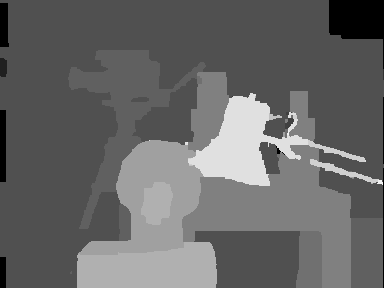
\includegraphics{pics/disparity.png}

\cvfunc{ReprojectImageTo3D}

Reprojects disparity image to 3D space.

\cvexp{

void cvReprojectImageTo3D( const CvArr* disparity,
                           CvArr* \_3dImage, const CvMat* Q );

}{CPP}{ReprojectImageTo3D(disparity,\_3dImage,Q)-> None}

\begin{description}
\cvarg{disparity}{Disparity map.}
\cvarg{\_3dImage}{3-channel, 16-bit integer or 32-bit floating-point image - the output map of 3D points.}
\cvarg{Q}{The reprojection 4x4 matrix.}
\end{description}

The function \texttt{cvReprojectImageTo3D} transforms 1-channel disparity map to 3-channel image, a 3D surface. That is, for each pixel \texttt{(x,y)} and the corresponding disparity d=disparity\texttt{(x,y)} it computes: 

$[X Y Z W]^T = Q*[x y d 1]^T
\newline
\_3dImage(x,y) = (X/W, Y/W, Z/W)$

The matrix Q can be arbitrary, e.g. the one, computed by \cross{cvStereoRectify}. To reproject a sparse set of points {(x,y,d),...} to 3D space, use \cross{cvPerspectiveTransform}. 

\section{Bibliography}
\begin{verbatim}
This bibliography provides a list of publications that were might be useful to the OpenCV users. This list is not complete; it serves only as a starting point.

 1. '''[Borgefors86]''' Gunilla Borgefors, "Distance Transformations in Digital Images". Computer Vision, Graphics and Image Processing 34, 344-371 (1986).
 1. '''[Bouguet00]''' Jean-Yves Bouguet. Pyramidal Implementation of the Lucas Kanade Feature Tracker.<<BR>> The paper is included into OpenCV distribution ([[attachment:algo\_tracking.pdf]])
 1. '''[Bradski98]''' G.R. Bradski. Computer vision face tracking as a component of a perceptual user interface. In Workshop on Applications of Computer Vision, pages 214?219, Princeton, NJ, Oct. 1998.<<BR>> Updated version can be found at http://www.intel.com/technology/itj/q21998/articles/art\_2.htm.<<BR>> Also, it is included into OpenCV distribution ([[attachment:camshift.pdf]])
 1. '''[Bradski00]''' G. Bradski and J. Davis. Motion Segmentation and Pose Recognition with Motion History Gradients. IEEE WACV'00, 2000.
 1. '''[Burt81]''' P. J. Burt, T. H. Hong, A. Rosenfeld. Segmentation and Estimation of Image Region Properties Through Cooperative Hierarchical Computation. IEEE Tran. On SMC, Vol. 11, N.12, 1981, pp. 802-809.
 1. '''[Canny86]''' J. Canny. A Computational Approach to Edge Detection, IEEE Trans. on Pattern Analysis and Machine Intelligence, 8(6), pp. 679-698 (1986).
 1. '''[Davis97]''' J. Davis and Bobick. The Representation and Recognition of Action Using Temporal Templates. MIT Media Lab Technical Report 402, 1997.
 1. '''[DeMenthon92]''' Daniel F. DeMenthon and Larry S. Davis. Model-Based Object Pose in 25 Lines of Code. In Proceedings of ECCV '92, pp. 335-343, 1992.
 1. '''[Fitzgibbon95]''' Andrew W. Fitzgibbon, R.B.Fisher. A Buyer?s Guide to Conic Fitting. Proc.5th British Machine Vision Conference, Birmingham, pp. 513-522, 1995.
 1. '''[Ford98]''' Adrian Ford, Alan Roberts. Colour Space Conversions. http://www.poynton.com/PDFs/coloureq.pdf
 1. '''[Horn81]''' Berthold K.P. Horn and Brian G. Schunck. Determining Optical Flow. Artificial Intelligence, 17, pp. 185-203, 1981.
 1. '''[Hu62]''' M. Hu. Visual Pattern Recognition by Moment Invariants, IRE Transactions on Information Theory, 8:2, pp. 179-187, 1962.
 1. '''[Iivarinen97]''' Jukka Iivarinen, Markus Peura, Jaakko Srel, and Ari Visa. Comparison of Combined Shape Descriptors for Irregular Objects, 8th British Machine Vision Conference, BMVC'97.<<BR>>http://www.cis.hut.fi/research/IA/paper/publications/bmvc97/bmvc97.html
 1. '''[Jahne97]''' B. Jahne. Digital Image Processing. Springer, New York, 1997.
 1. '''[Lucas81]''' Lucas, B., and Kanade, T. An Iterative Image Registration Technique with an Application to Stereo Vision, Proc. of 7th International Joint Conference on Artificial Intelligence (IJCAI), pp. 674-679.
 1. '''[Kass88]''' M. Kass, A. Witkin, and D. Terzopoulos. Snakes: Active Contour Models, International Journal of Computer Vision, pp. 321-331, 1988.
 1. '''[Lienhart02]''' Rainer Lienhart and Jochen Maydt. An Extended Set of Haar-like Features for Rapid Object Detection. IEEE ICIP 2002, Vol. 1, pp. 900-903, Sep. 2002.<<BR>> This paper, as well as the extended technical report, can be retrieved at http://www.lienhart.de/Publications/publications.html
 1. '''[Matas98]''' J.Matas, C.Galambos, J.Kittler. Progressive Probabilistic Hough Transform. British Machine Vision Conference, 1998.
 1. '''[Rosenfeld73]''' A. Rosenfeld and E. Johnston. Angle Detection on Digital Curves. IEEE Trans. Computers, 22:875-878, 1973.
 1. '''[RubnerJan98]''' Y. Rubner. C. Tomasi, L.J. Guibas. Metrics for Distributions with Applications to Image Databases. Proceedings of the 1998 IEEE International Conference on Computer Vision, Bombay, India, January 1998, pp. 59-66.
 1. '''[RubnerSept98]''' Y. Rubner. C. Tomasi, L.J. Guibas. The Earth Mover?s Distance as a Metric for Image Retrieval. Technical Report STAN-CS-TN-98-86, Department of Computer Science, Stanford University, September 1998.
 1. '''[RubnerOct98]''' Y. Rubner. C. Tomasi. Texture Metrics. Proceeding of the IEEE International Conference on Systems, Man, and Cybernetics, San-Diego, CA, October 1998, pp. 4601-4607. http://robotics.stanford.edu/~rubner/publications.html
 1. '''[Serra82]''' J. Serra. Image Analysis and Mathematical Morphology. Academic Press, 1982.
 1. '''[Schiele00]''' Bernt Schiele and James L. Crowley. Recognition without Correspondence Using Multidimensional Receptive Field Histograms. In International Journal of Computer Vision 36 (1), pp. 31-50, January 2000.
 1. '''[Suzuki85]''' S. Suzuki, K. Abe. Topological Structural Analysis of Digital Binary Images by Border Following. CVGIP, v.30, n.1. 1985, pp. 32-46.
 1. '''[Teh89]''' C.H. Teh, R.T. Chin. On the Detection of Dominant Points on Digital Curves. - IEEE Tr. PAMI, 1989, v.11, No.8, p. 859-872.
 1. '''[Trucco98]''' Emanuele Trucco, Alessandro Verri. Introductory Techniques for 3-D Computer Vision. Prentice Hall, Inc., 1998.
 1. '''[Viola01]''' Paul Viola and Michael J. Jones. Rapid Object Detection using a Boosted Cascade of Simple Features. IEEE CVPR, 2001.<<BR>> The paper is available online at http://www.ai.mit.edu/people/viola/
 1. '''[Welch95]''' Greg Welch, Gary Bishop. An Introduction To the Kalman Filter. Technical Report TR95-041, University of North Carolina at Chapel Hill, 1995.<<BR>> Online version is available at http://www.cs.unc.edu/~welch/kalman/kalmanIntro.html
 1. '''[Williams92]''' D. J. Williams and M. Shah. A Fast Algorithm for Active Contours and Curvature Estimation. CVGIP: Image Understanding, Vol. 55, No. 1, pp. 14-26, Jan., 1992. http://www.cs.ucf.edu/~vision/papers/shah/92/WIS92A.pdf.
 1. '''[Yuen03]''' H.K. Yuen, J. Princen, J. Illingworth and J. Kittler. Comparative study of Hough Transform methods for circle finding.<<BR>>http://www.sciencedirect.com/science/article/B6V09-48TCV4N-5Y/2/91f551d124777f7a4cf7b18325235673
 1. '''[Yuille89]''' A.Y.Yuille, D.S.Cohen, and P.W.Hallinan. Feature Extraction from Faces Using Deformable Templates in CVPR, pp. 104-109, 1989.
 1. '''[Zhang96]''' Z. Zhang. Parameter Estimation Techniques: A Tutorial with Application to Conic Fitting, Image and Vision Computing Journal, 1996.
 1. '''[Zhang99]''' Z. Zhang. Flexible Camera Calibration By Viewing a Plane From Unknown Orientations. International Conference on Computer Vision (ICCV'99), Corfu, Greece, pages 666-673, September 1999.
 1. '''[Zhang00]''' Z. Zhang. A Flexible New Technique for Camera Calibration. IEEE Transactions on Pattern Analysis and Machine Intelligence, 22(11):1330-1334, 2000.
\end{verbatim}
